\documentclass[11pt,oneside]{book}
\usepackage{fontspec}
\setmainfont{Noto Serif}
\setsansfont{Noto Sans}
\setmonofont{Noto Sans Mono}
\newfontfamily\proseunicodefont{DejaVu Serif}
\usepackage[margin=1in]{geometry}
\usepackage{microtype}
\usepackage{amsmath,amssymb,amsthm,mathtools,bm}
\usepackage{graphicx}
\usepackage{xcolor}
\usepackage{booktabs}
\usepackage{array}
\usepackage{longtable}
\usepackage{enumitem}
\usepackage{float}
\usepackage{caption}
\usepackage{hyperref}
\usepackage{fancyhdr}
\usepackage{tikz}
\usetikzlibrary{arrows.meta,positioning,calc,decorations.pathmorphing}

\hypersetup{
  colorlinks=true,
  linkcolor=blue!50!black,
  urlcolor=blue!50!black,
  citecolor=blue!50!black
}

\setlength{\parskip}{0.5em}
\setlength{\parindent}{0pt}
\setlist[itemize]{topsep=0.25em,itemsep=0.2em}
\setlist[enumerate]{topsep=0.25em,itemsep=0.2em}
\setlength{\headheight}{40pt}
\numberwithin{equation}{chapter}

\newtheorem{theorem}{Định lý}[chapter]
\newtheorem{proposition}[theorem]{Mệnh đề}
\newtheorem{lemma}[theorem]{Bổ đề}
\newtheorem{corollary}[theorem]{Hệ quả}
\theoremstyle{definition}
\newtheorem{definition}[theorem]{Định nghĩa}
\newtheorem{example}[theorem]{Ví dụ}
\theoremstyle{remark}
\newtheorem{remark}[theorem]{Nhận xét}

\providecommand{\ket}[1]{\left\lvert#1\right\rangle}
\providecommand{\bra}[1]{\left\langle#1\right\rvert}
\providecommand{\braket}[2]{\left\langle#1\,\middle|\,#2\right\rangle}
\providecommand{\expect}[1]{\left\langle#1\right\rangle}
\newcommand{\lectureoverview}[1]{\paragraph{Tổng quan.} #1}
\newenvironment{classroomqa}{%
  \par\medskip
  \begin{minipage}{0.96\textwidth}
}{%
  \end{minipage}
  \par\medskip
}
\newcommand{\audiencequestion}[1]{\noindent\textbf{Câu hỏi từ người nghe.} #1\par\smallskip}
\newcommand{\lecturerresponse}[1]{\noindent\textbf{Trả lời.} #1\par}
\newcommand{\lecturetimestamp}[1]{\footnote{Mốc thời gian bài giảng: #1.}}
\newcommand{\lectureframe}[1]{\par\smallskip{\centering\footnotesize\itshape Khung hình bài giảng: #1.\par}}
\newcommand{\editorialnote}[1]{\footnote{Chú giải biên tập: #1}}

\makeatletter
\newcommand{\course@headerfont}{\normalfont\small\itshape}
\newcommand{\course@pagefont}{\normalfont\small}
\newcommand{\course@headerraise}{14pt}
\newlength{\course@headerboxheight}
\setlength{\course@headerboxheight}{\dimexpr\headheight-\course@headerraise-9pt\relax}
\newcommand{\course@leftheadbox}[1]{%
  \raisebox{\course@headerraise}{%
    \parbox[t][\course@headerboxheight][t]{0.82\textwidth}{%
      \raggedright\course@headerfont\strut\MakeUppercase{#1}\strut%
    }%
  }%
}
\newcommand{\course@rightheadbox}[1]{%
  \raisebox{\course@headerraise}{%
    \parbox[t][\course@headerboxheight][t]{0.82\textwidth}{%
      \raggedleft\course@headerfont\strut\MakeUppercase{#1}\strut%
    }%
  }%
}
\renewcommand{\chaptermark}[1]{\markboth{\MakeUppercase{\chaptername\ \thechapter.\ #1}}{}}
\renewcommand{\sectionmark}[1]{\markright{\MakeUppercase{\thesection\hspace{0.4em}#1}}}
\fancyhf{}
\fancyhead[L]{\course@leftheadbox{\leftmark}}
\fancyhead[R]{\course@pagefont\thepage}
\renewcommand{\headrulewidth}{0.5pt}
\pagestyle{fancy}
\fancypagestyle{plain}{%
  \fancyhf{}
  \fancyhead[L]{\course@leftheadbox{\leftmark}}
  \fancyhead[R]{\course@pagefont\thepage}
  \renewcommand{\headrulewidth}{0.5pt}
}
\makeatother

\usepackage{polyglossia}
\setdefaultlanguage{vietnamese}
\usepackage{sectsty}
\renewcommand{\contentsname}{Mục lục}
\renewcommand{\chaptername}{Chương}
\renewcommand{\figurename}{Hình}
\renewcommand{\tablename}{Bảng}
\renewcommand{\proofname}{Chứng minh}
\renewcommand{\bibname}{Tài liệu tham khảo}
\sectionfont{\raggedright}
\subsectionfont{\raggedright}
\makeatletter
\renewcommand{\@pnumwidth}{2.2em}
\renewcommand{\@tocrmarg}{3.2em}
\makeatother
\usepackage{tocloft}
\renewcommand{\cftchapfont}{\small\bfseries}
\renewcommand{\cftchappagefont}{\small\bfseries}
\renewcommand{\cftsecfont}{\small}
\renewcommand{\cftsecpagefont}{\small}
\setlength{\cftsecnumwidth}{3em}
\renewcommand{\cftsubsecfont}{\small}
\renewcommand{\cftsubsecpagefont}{\small}
\setlength{\cftsubsecindent}{4.5em}
\setlength{\cftsubsecnumwidth}{4em}
\emergencystretch=6em
\pdfstringdefDisableCommands{\def\proseunicodefont{}}

\geometry{paperwidth=177.6mm,paperheight=252mm,left=16mm,right=16mm,
 top=18mm,bottom=18mm,includeheadfoot,headheight=28pt,headsep=7mm,footskip=9mm}
\usepackage{scrextend}
\changefontsizes[17pt]{12pt}
\raggedbottom
\renewenvironment{classroomqa}{\par\medskip\begingroup}{\par\endgroup\medskip}
\fancyhf{}
\setlength{\headwidth}{\textwidth}
\fancyhead[L]{\parbox{\textwidth}{\raggedright\fontsize{9}{11}\selectfont\nouppercase{\leftmark}}}
\fancyfoot[C]{\small\thepage}
\renewcommand{\headrulewidth}{0.3pt}
\fancypagestyle{plain}{\fancyhf{}\fancyfoot[C]{\small\thepage}\renewcommand{\headrulewidth}{0pt}}

\hypersetup{
  pdftitle={Quantum Entanglement, Part 3},
  pdfauthor={Lectures by Leonard Susskind; companion edition by LazyingArt LLC},
  pdfsubject={Independently edited companion notes for the 2006 Fall lecture course},
  pdfcreator={LaTeX with hyperref}
}
\graphicspath{{../../../generated_course_notes/supplementary/quantum_entanglement/2006_fall_part_3/figures/}{../../../generated_course_notes/supplementary/quantum_entanglement/2006_fall_part_3/assets/}}
\begin{document}
\frontmatter
\hypersetup{pageanchor=false}
\begin{titlepage}
\hyphenpenalty=10000\exhyphenpenalty=10000
\thispagestyle{empty}
\begin{tikzpicture}[remember picture,overlay]
  \node[anchor=center,inner sep=0] at (current page.center) {%
    \includegraphics[height=\paperheight,keepaspectratio]{../../../generated_course_notes/supplementary/quantum_entanglement/2006_fall_part_3/assets/cover-art.png}%
  };
  \node[
    anchor=north west,
    align=left,
    text width=0.78\paperwidth,
    fill=white,
    fill opacity=0.9,
    rounded corners=8pt,
    inner xsep=10pt,
    inner ysep=8pt
  ] at ([xshift=0.08\paperwidth,yshift=-0.06\paperheight]current page.north west) {%
    {\fontsize{30}{33}\selectfont\bfseries\color{black!88} Rối lượng tử, Phần 3\\[0.85em]}
    {\large\color{black!72} Bản tiếng Việt / mùa thu 2006, phần 3}
  };
  \node[
    anchor=south west,
    align=left,
    text width=0.68\paperwidth,
    fill=white,
    fill opacity=0.82,
    text opacity=1,
    rounded corners=6pt,
    inner sep=12pt
  ] at ([xshift=0.08\paperwidth,yshift=0.08\paperheight]current page.south west) {%
    {\normalsize\color{black!78} Bài giảng gốc: Leonard Susskind\\[0.35em]}
    {\small\color{black!72} Ấn bản đồng hành: \href{https://lazying.art}{LazyingArt LLC} / \href{https://github.com/lachlanchen/Video2Book}{Video2Book}}
  };
\end{tikzpicture}
\mbox{}
\end{titlepage}
\hypersetup{pageanchor=true}

\clearpage
\chapter*{Về các ghi chú này}
Các ghi chú đồng hành được biên tập độc lập này bám theo phần thứ ba của khóa bài giảng năm 2006 của Leonard Susskind về rối lượng tử. Chúng được phục dựng từ các bản chép lời do máy tạo, phụ đề và những khung hình bảng viết được chọn lọc, rồi được đối chiếu với các tư liệu nguồn hiện có. Chúng không phải là bản thảo gốc của Giáo sư Susskind và cũng chưa được ông xem xét hay chấp thuận.

Ấn bản này được \href{https://lazying.art}{LazyingArt LLC} biên soạn bằng bộ công cụ nguồn mở \href{https://github.com/lachlanchen/Video2Book}{Video2Book}. Các bản chép lời do máy tạo vẫn được cung cấp riêng và có thể chứa lỗi nhận dạng. Các chỗ làm rõ của biên tập viên và những phần phục dựng không tầm thường được chỉ rõ trong chú thích chân trang.
\clearpage
\tableofcontents
\mainmatter
\chapter{Thuyết tương đối hẹp: các hệ quy chiếu, tính đồng thời và phép biến đổi Lorentz}

Thuyết tương đối là nguyên lý cho rằng các định luật vật lý không phụ thuộc vào việc ta dùng hệ quy chiếu quán tính nào để mô tả chúng. Nhiệm vụ đầu tiên của chúng ta là động học: ý nghĩa của không gian, thời gian, chuyển động, sự đồng bộ hóa, và phép biến đổi từ một hệ quy chiếu quán tính sang một hệ khác. Động lực học đến sau, với năng lượng tương đối tính, động lượng, lực, dạng tương tự của phương trình chuyển động Newton, và ý nghĩa của \(E=mc^2\). Một khi cấu trúc đó đã vững chắc, ta có thể tiếp cận thuyết tương đối rộng về mặt khái niệm thông qua không-thời gian cong, chuyển động của các hạt trong một trường hấp dẫn cho trước, các lỗ đen, và sự giãn nở của vũ trụ, mà không cần bắt đầu từ bài toán khó là giải các phương trình trường Einstein.

Cần phân biệt giữa tính chặt chẽ về mặt khái niệm và về mặt toán học. Chúng ta sẽ không dùng một phép gần đúng mà ta biết là sai. Thay vào đó, ta sẽ nhấn mạnh trường hấp dẫn tác động lên đồng hồ, hạt và hình học như thế nào, đồng thời hoãn lại bộ công cụ cần để xây dựng các nghiệm tùy ý của phương trình trường. Thuyết tương đối hẹp phải được trình bày tường minh hơn vì toàn bộ lập luận về sau đều dựa trên động học của nó.

Vì vậy, điểm khởi đầu đúng không phải là một công thức nổi tiếng, mà là một trình bày chính xác về điều mà một người quan sát hiểu là một vị trí và một thời điểm.

\section{Một hệ quy chiếu là một hệ tọa độ vật lý}

Hãy hình dung không gian được lấp đầy bởi một mạng gồm các thước mét mịn đến mức tùy ý. Mỗi nút mạng được gán ba tọa độ không gian, và tại mỗi nút đều có một đồng hồ. Gộp lại, các thước và các đồng hồ ấy tạo thành một hệ quy chiếu.

\begin{definition}
Một \emph{biến cố} là một điều xảy ra tại một vị trí và một thời điểm. Trong một chiều không gian, tọa độ của nó được viết là \((x,t)\); trong ba chiều, chúng là \((x,y,z,t)\).
\end{definition}

Vật lý Newton bổ sung một giả thiết mạnh: mọi đồng hồ lý tưởng đều có thể được đồng bộ hóa một lần là mãi mãi. Thời gian là phổ quát. Một đồng hồ có thể được di chuyển, và một người quan sát có thể mang theo đồng hồ đeo tay, nhưng mọi người đều được giả định là thống nhất về cùng một \(t\) ở mọi nơi. Điều này đôi khi được gọi là thời gian tuyệt đối; ta có thể hình dung nó như thời gian của Thượng đế, một chiếc đồng hồ duy nhất cho toàn thế giới.

Nguyên lý tương đối có trước Einstein. Hình ảnh tự nhiên của nó là một đoàn tàu chuyển động đều đến mức trên đường ray hoàn toàn nhẵn không có gì rung lắc hay xóc nảy. Bên trong tàu, ta có thể tung và bắt các quả bóng đúng như khi ở một đoàn tàu đang đứng tại ga. Trò tung hứng là một thí nghiệm cơ học nhỏ nhưng đầy đủ một cách đáng ngạc nhiên: nó đòi hỏi việc canh thời gian, trọng lực, sự căn chỉnh, và khả năng điều khiển lặp đi lặp lại các quỹ đạo. Nếu tàu chuyển động với vận tốc không đổi, không quy tắc nào trong số đó thay đổi. Một quả bóng ném thẳng lên trên sẽ trở lại đúng bàn tay cũ; đoàn tàu không trượt đi khỏi ngay bên dưới nó. Galileo nhận ra điều này, và Newton diễn đạt nó một cách có hệ thống trong các định luật chuyển động của mình.

Trước Galileo, người ta dễ bị cám dỗ lập luận rằng đoàn tàu đang chạy hẳn phải tiến lên trong lúc quả bóng còn ở trên không, buộc người tung hứng phải với tay ra sau hoặc ra trước để bắt lại nó. Sai lầm là quên rằng quả bóng đã mang sẵn vận tốc ngang của đoàn tàu khi rời tay. Không thí nghiệm nào bị giới hạn trong toa tàu chuyển động êm lại bộc lộ một trạng thái nghỉ tuyệt đối đặc biệt. Chỉ có chuyển động tương đối giữa hai đoàn tàu là quan sát được.

Vì thế, đoàn tàu đứng yên và đoàn tàu chuyển động đều là hai hệ quy chiếu quán tính. Trước Einstein, chúng liên hệ với nhau bằng các phép biến đổi Galileo.

\section{Vẽ không-thời gian}

Tạm thời ta bỏ qua \(y\) và \(z\), vẽ thời gian theo phương thẳng đứng và vị trí \(x\) theo phương ngang. Mỗi điểm trong hình vẽ là một biến cố. Đường \(x=0\) là lịch sử, hay \emph{đường thế giới}, của gốc không gian. Các đường thẳng đứng lân cận \(x=1,2,3,\ldots\) là các đường thế giới của những nút mạng khác. Các đường ngang là tập hợp các biến cố có cùng một thời gian.

\begin{figure}[H]
\centering
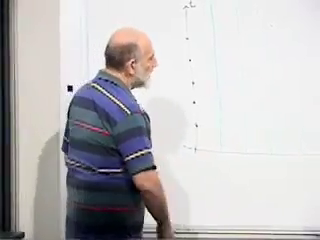
\includegraphics[width=0.62\textwidth]{lecture_01_figure_02.png}
\caption{Trục thời gian của hệ nghỉ và các đường thế giới đầu tiên của mạng không gian.}
\lectureframe{00:16:38}
\end{figure}

Cùng một cách dựng ấy sẽ rõ hơn trong một hình vẽ lý tưởng hóa:

\begin{figure}[H]
\centering
\begin{tikzpicture}[scale=0.95]
\draw[->] (-1.2,0) -- (5.2,0) node[right] {$x$};
\draw[->] (0,-0.2) -- (0,4.8) node[above] {$t$};
\foreach \x in {-1,1,2,3,4}
  \draw[gray!65] (\x,0) -- (\x,4.4);
\foreach \y in {1,2,3,4}
  \draw[gray!65] (-1.0,\y) -- (4.4,\y);
\fill (0,0) circle (1.5pt);
\node[below left] at (0,0) {$0$};
\node[left] at (0,1) {$1$};
\node[left] at (0,2) {$2$};
\node[left] at (0,3) {$3$};
\node[below] at (1,0) {$1$};
\node[below] at (2,0) {$2$};
\node[below] at (3,0) {$3$};
\end{tikzpicture}
\caption{Một mạng không-thời gian đứng yên. Các đường thẳng đứng có vị trí không đổi; các đường ngang có thời gian không đổi.}
\end{figure}

Lưới này là tưởng tượng, và khoảng cách mắt lưới là tùy ý. Ta có thể dùng mét, xentimét, micrômét, hoặc bất kỳ khoảng nhỏ hơn nào nữa mà vẫn có ý nghĩa vật lý. Mục đích của nó là gán một tọa độ chính xác cho mọi biến cố.

Cụm từ “hệ quy chiếu” giờ đây có nội dung thao tác rõ ràng. Nó không chỉ đơn thuần là một góc nhìn hay một người đang nhìn theo hướng nào đó. Nó là một bộ máy tọa độ mở rộng. Với một biến cố cho trước, các thước cục bộ xác định nó xảy ra ở đâu và đồng hồ cục bộ xác định nó xảy ra khi nào. Khi đó ta có thể so sánh các đại lượng vật lý khác giữa các hệ: vị trí và vận tốc của một hạt, năng lượng của nó, có lẽ là nhiệt độ của một vật, và về sau là động lượng và lực của nó. So sánh đơn giản nhất là so sánh liên quan đến \(x\) và \(t\), nên ta bắt đầu từ đó.

Bây giờ đặt một mạng thứ hai trên một đoàn tàu đang chuyển động theo chiều dương của \(x\) với vận tốc không đổi \(v\). Chọn sao cho hai gốc trùng nhau tại \(t=0\). Khi đó gốc chuyển động tuân theo
\begin{equation}
x=vt.
\end{equation}
Mọi điểm khác cố định trên tàu đi theo một đường thế giới nghiêng song song. Độ nghiêng chỉ đơn giản là phát biểu hình học rằng đoàn tàu đổi vị trí khi thời gian trôi qua.

Giả sử điểm phía sau của đoàn tàu là gốc của hệ có phẩy. Tại \(t=0\) nó trùng với gốc của ga. Ở một thời điểm muộn hơn \(t\), tọa độ của nó trong hệ đứng yên là \(vt\). Vì vậy, một biến cố gần đó có tọa độ \(x\) chỉ cách gốc của đoàn tàu một đoạn \(x-vt\). Đây là lý do phép biến đổi là một phép trừ chứ không phải một quy tắc đại số tùy tiện.

Gọi \((x,t)\) là các tọa độ của một biến cố trong hệ của ga và \((x',t')\) là các tọa độ của nó trong hệ của đoàn tàu. Galileo và Newton giữ thời gian phổ quát,
\begin{equation}
t'=t.
\end{equation}
Trong khoảng thời gian \(t\), gốc chuyển động tiến thêm \(vt\), nên khoảng cách từ gốc ấy đến biến cố là
\begin{equation}
x'=x-vt.
\end{equation}
Gộp lại,
\begin{align}
t'&=t, & x'&=x-vt.
\label{eq:galilean-forward}
\end{align}
Giải theo các tọa độ không phẩy cho ta phép biến đổi nghịch,
\begin{align}
t&=t', & x&=x'+vt'.
\label{eq:galilean-inverse}
\end{align}

\begin{figure}[H]
\centering
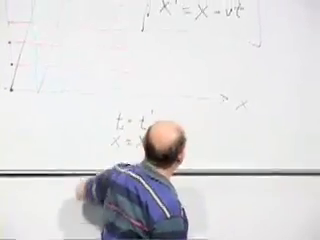
\includegraphics[width=0.72\textwidth]{lecture_01_figure_03.png}
\caption{Phép biến đổi Galileo được viết bên cạnh hai mạng không-thời gian.}
\lectureframe{00:21:57}
\end{figure}

Cặp thứ nhất cho người quan sát chuyển động biết cách chuyển đổi các tọa độ do người quan sát đứng yên cung cấp. Cặp nghịch đảo chuyển đổi theo chiều ngược lại. Sự chuyển đổi hai chiều qua lại giữa các mô tả này là nội dung toán học của thuyết tương đối Galileo.

Việc thay \(t\to t'\) trong công thức không gian nghịch là vô hại chỉ vì lý thuyết Galileo đã tuyên bố sẵn \(t=t'\). Bây giờ lưu ý giả thiết ấy là điều hữu ích. Trong lý thuyết của Einstein, hai tọa độ thời gian sẽ khác nhau, và những phép thay thế như vậy sẽ không còn tự động nữa.

\begin{classroomqa}
\audiencequestion{Nếu mang một đồng hồ đi xa rồi đem trở lại, làm sao ta biết rằng chuyển động của nó không phải là lúc đầu làm nó chạy nhanh hơn rồi sau đó làm nó chạy chậm lại, che lấp hiệu ứng khi so sánh các đồng hồ?
\lecturetimestamp{00:23:09}}
\lecturerresponse{Galileo không thể xác lập thời gian phổ quát với độ chính xác hiện đại; đó là một phỏng đoán vật lý. Ta có thể kiểm tra phỏng đoán ấy bằng nhiều cách: mang các đồng hồ tốt đi theo hai hướng ngược nhau, lặp lại chuyến đi theo hướng bắc--nam cũng như đông--tây, cho một đồng hồ chuyển động vòng quanh chiếc kia, hoặc trao đổi các tín hiệu định thời mà không cần đưa các đồng hồ lại gần nhau. Ở các tốc độ thông thường, mọi phép kiểm tra như vậy đều phù hợp với nhau với độ chính xác rất cao. Với các đồng hồ đủ chính xác hoặc các tốc độ đủ lớn, một sai khác nhỏ quả thật xuất hiện. Việc thời gian phổ quát không còn đúng không phải là khuyết điểm của thí nghiệm; nó là một trong những hiện tượng mà thuyết tương đối hẹp phải giải thích.}
\end{classroomqa}

\section{Các bất biến Galileo và định luật Newton}

Một bất biến là một đại lượng mà mọi người quan sát quán tính đang được xét đều thống nhất. Bản thân các tọa độ không nhất thiết phải bất biến. Điều quan trọng là liệu các định luật được xây dựng từ chúng có giữ nguyên cùng một dạng hay không.

Từ này được dùng vừa như danh từ vừa như tính từ. Một con số có thể là một bất biến, và một phương trình có thể bất biến dưới một phép biến đổi. Sự phân biệt giữa các đại lượng bất biến và các định luật bất biến ngăn ngừa một sự nhầm lẫn thường gặp: thuyết tương đối không khẳng định rằng mọi người quan sát đều thu được cùng một tọa độ cho mọi thứ. Nó khẳng định rằng định luật vật lý nối các phép đo của họ có cùng một dạng.

Xét hai biến cố đồng thời tại các vị trí \(x_1\) và \(x_2\). Phương trình~\eqref{eq:galilean-forward} cho
\begin{align}
x_1'&=x_1-vt,\\
x_2'&=x_2-vt.
\end{align}
Vì thế khoảng cách giữa chúng là
\begin{equation}
x_2'-x_1'=(x_2-vt)-(x_1-vt)=x_2-x_1.
\end{equation}
Trong vật lý Galileo, khoảng cách giữa các biến cố xảy ra cùng một thời gian là bất biến mặc dù từng vị trí riêng lẻ thì không.

\begin{classroomqa}
\audiencequestion{Hai lần xuất hiện của \(t\) trong phép trừ đó có thật sự là cùng một thời gian không?
\lecturetimestamp{00:28:16}}
\lecturerresponse{Có. Ta đã cố ý chọn hai biến cố là \((x_1,t)\) và \((x_2,t)\). Chúng nằm trên cùng một đường ngang thời gian không đổi. Vì vậy hạng chung \(vt\) triệt tiêu. Nếu các biến cố xảy ra ở những thời gian khác nhau, lập luận này sẽ không thiết lập được một khoảng cách không gian bất biến.}
\end{classroomqa}

Bây giờ mô tả một hạt bằng quỹ đạo \(x(t)\). Người quan sát trên tàu gán
\begin{equation}
x'(t)=x(t)-vt.
\end{equation}
Lấy đạo hàm một lần cho quy tắc cộng vận tốc quen thuộc,
\begin{equation}
\frac{dx'}{dt}=\frac{dx}{dt}-v.
\end{equation}
Vị trí và vận tốc phụ thuộc hệ quy chiếu. Một người quan sát chuyển động song song với một mũi tên sẽ thấy nó bay chậm hơn so với người quan sát đứng bên đường ray.

Lấy đạo hàm thêm lần nữa. Vì vận tốc tương đối \(v\) là hằng số,
\begin{equation}
\frac{d^2x'}{dt^2}=\frac{d^2x}{dt^2}.
\end{equation}
Gia tốc là bất biến dưới một phép biến đổi Galileo. Điều này gợi ý mạnh vì sao định luật Newton được viết theo gia tốc chứ không theo vị trí hay vận tốc.

Đây là gia tốc của vật được quan sát, không phải gia tốc của người quan sát trên tàu. Cả hai hệ đều là quán tính, nên không hệ nào gia tốc so với hệ kia. Các vật có thể gia tốc sang trái hoặc sang phải trong bất kỳ mô tả nào, và hai người quan sát đều nhất trí về giá trị của gia tốc ấy mặc dù họ bất đồng về vị trí và vận tốc của vật.

Giả sử hai hạt tác dụng lực lên nhau và lực chỉ phụ thuộc vào khoảng cách đồng thời giữa chúng. Khoảng cách ấy là bất biến, nên lực là bất biến. Nếu khối lượng cũng là một tính chất nội tại, độc lập với hệ quy chiếu, thì mọi người quan sát quán tính đều có thể viết
\begin{equation}
F=ma
\end{equation}
ở đúng cùng một dạng. Cơ học Newton là bất biến dưới các phép biến đổi Galileo. Điều đó không chỉ là điều có vẻ hợp lý; trong toàn bộ miền tốc độ thông thường, nó cực kỳ chính xác.

Lập luận này áp dụng cho các lực trung tâm quen thuộc như hấp dẫn Newton hay tĩnh điện học, trong đó độ lớn là một hàm của khoảng cách. Vì mọi người quan sát trong cơ học Galileo đều thống nhất về khoảng cách ấy tại cùng một thời gian, họ thống nhất về lực. Khi lực và gia tốc đã cố định, tính nhất quán khi đó buộc họ cũng phải thống nhất về khối lượng: một vật một kilôgam vẫn là một vật một kilôgam khi được chở ngang qua trên một đoàn tàu. Mọi ký hiệu trong \(F=ma\) đều phù hợp với cùng một cấu trúc bất biến.

\section{Ánh sáng không phù hợp với quy tắc Galileo}

Điện từ học gây ra khó khăn. Các phương trình Maxwell dự đoán những sóng truyền qua không gian rỗng với tốc độ xác định \(c\). Nếu các phương trình Maxwell là các định luật tự nhiên và các định luật tự nhiên là như nhau trong mọi hệ quy chiếu quán tính, thì mọi người quan sát quán tính đều phải thu được cùng một \(c\).

Động học Galileo lại dự đoán điều khác. Một xung ánh sáng truyền sang phải trong hệ đứng yên thỏa mãn
\begin{equation}
x=ct.
\end{equation}
Áp dụng phép biến đổi không gian cho ta
\begin{equation}
x'=x-vt=(c-v)t.
\end{equation}
Vì \(t'=t\), người quan sát trên tàu sẽ đo được tốc độ \(c-v\).

Mâu thuẫn có thể được phát biểu dứt khoát. Nếu các phương trình Maxwell giữ nguyên dạng của chúng, chúng dự đoán \(c\) trong hệ có phẩy. Nếu vẫn giữ phép biến đổi Galileo, nó dự đoán \(c-v\). Không thể cả hai đều đúng một cách chính xác khi \(v\ne0\).

Kết quả này trông hoàn toàn tự nhiên nếu ánh sáng ứng xử như một sóng thông thường trong một môi trường. Một chiếc thuyền chuyển động cùng với sóng nước sẽ đo được tốc độ tương đối của sóng thấp hơn. Một người nghe chuyển động trong không khí đứng yên sẽ đo được một tốc độ âm thanh bị dịch đi bởi chuyển động của người đó so với không khí. Vì thế, các nhà vật lý thế kỷ 19 đã đi đến một trạng thái đứng yên ưu tiên, một hệ quy chiếu ête trong đó các phương trình Maxwell có dạng đơn giản nhất và ánh sáng truyền với tốc độ \(c\). Các thí nghiệm được thiết kế để phát hiện chuyển động tương đối so với một hệ quy chiếu ưu tiên như vậy đã không tìm thấy hiệu ứng tương ứng nào.

Có một số cách bố trí thí nghiệm khả dĩ, nhưng mục tiêu chung của chúng là so sánh sự truyền ánh sáng đối với các quan sát viên ở những trạng thái hoặc phương chuyển động khác nhau. Không thí nghiệm nào cho thấy độ dịch Galile như mong đợi. Sự thất bại đó không phải là một phiền toái kỹ thuật nhỏ nhặt. Nó buộc người ta phải lựa chọn giữa nguyên lý tương đối, các phương trình Maxwell và những quan niệm được thừa hưởng về không gian và thời gian.

Einstein tiếp cận xung đột này một cách trực diện hơn. Khi còn trẻ, ông hình dung mình đuổi theo một sóng ánh sáng. Nếu ông có thể bắt kịp nó, mẫu điện từ dao động của nó sẽ đứng yên đông cứng trong không gian, thế nhưng các phương trình Maxwell không cho phép một sóng ánh sáng đứng yên như vậy. Ông chọn xem lý thuyết Maxwell và nguyên lý tương đối là nền tảng, rồi xem xét lại những giả thiết ẩn trong các tọa độ của chúng ta.

Sự xây dựng lại này dựa trên hai tiên đề:
\begin{enumerate}
\item Các định luật vật lý có cùng dạng trong mọi hệ quy chiếu quán tính.
\item Ánh sáng trong chân không có cùng tốc độ \(c\) trong mọi hệ quy chiếu quán tính.
\end{enumerate}

Tiên đề thứ hai không thể cùng tồn tại với phép biến đổi Galile. Phải thay đổi một điều gì đó sâu hơn quy tắc cộng vận tốc. Lựa chọn tối giản của Einstein là giữ lại hai tiên đề ấy và xem xét lại phương trình Galile tưởng như vô hại \(t'=t\).

\section{Đồng bộ hóa các đồng hồ ở xa}

Các khoảng cách trong không gian có thể được xác lập bằng các thanh đo, nhưng các đồng hồ ở xa đòi hỏi một quy ước đồng bộ hóa. Đặt hai đồng hồ ở những khoảng cách bằng nhau đối với một quan sát viên ở trung điểm. Khi mỗi đồng hồ ở đầu mút chỉ đúng thời điểm đã định, hãy để nó phát ra một chớp sáng. Nếu hai chớp sáng đến trung điểm cùng lúc, hãy gọi hai đồng hồ ở đầu mút là đã đồng bộ. Nếu một chớp đến trước, hãy điều chỉnh đồng hồ tương ứng rồi lặp lại quy trình.

Từ \emph{trung điểm} được định nghĩa bằng các thanh đo đã được đặt ra trong chính hệ đó. Vì vậy, phép kiểm tra này chứa hai thành phần tách biệt: khoảng cách không gian bằng nhau tới hai đầu mút và thời điểm đến bằng nhau của các tín hiệu. Không thể bỏ đi thành phần nào. Lặp lại quy trình ấy trên toàn bộ mạng lưới sẽ cho các đường ngang thời gian không đổi mà Newton chỉ đơn giản giả định sẵn.

Định nghĩa này dùng ánh sáng vì tiên đề gán cho ánh sáng cùng một tốc độ trong mọi hệ quy chiếu quán tính. Khi mọi cặp lân cận đều đã được xử lý theo cách này, toàn bộ mạng lưới sẽ mang một hệ đồng hồ đồng bộ.

Bây giờ hãy để một mạng lưới thứ hai chuyển động qua mạng thứ nhất. Trung điểm của thiết bị chuyển động vẫn nằm đúng giữa hai đầu mút đang chuyển động của nó trong chính hệ của nó. Tuy nhiên, so với thiết bị đứng yên, nó chuyển động về phía một chớp tới và rời xa chớp kia. Những chớp được phát ra đồng thời theo các đồng hồ đứng yên không đến cùng lúc tại trung điểm đang chuyển động. Vì quan sát viên chuyển động áp dụng cùng quy tắc trung điểm-và-ánh sáng, nên người đó không thể gọi những lần phát ấy là đồng thời. Mỗi hệ tự đồng bộ hóa các đồng hồ của mình một cách nhất quán, nhưng hai cách đồng bộ đó bất đồng với nhau.

Đây không phải là một ảo giác quang học do thời gian truyền hữu hạn của ánh sáng gây ra. Mỗi quan sát viên đều biết rằng ánh sáng cần thời gian để tới nơi và hiệu chỉnh điều đó bằng cùng tốc độ \(c\). Sự bất đồng vẫn còn sau hiệu chỉnh ấy vì các quan sát viên không chọn cùng một cặp sự kiện ở xa làm một cặp đồng thời. Chính tính đồng thời, chứ không chỉ vẻ bề ngoài của tính đồng thời, là tương đối.

\begin{classroomqa}
\audiencequestion{Liệu ta có thể tránh kết luận này bằng cách đồng bộ hóa đồng hồ bằng âm thanh thay vì bằng ánh sáng không?
\lecturetimestamp{00:49:03}}
\lecturerresponse{Âm thanh dùng được như một tín hiệu đồng bộ hóa trong một hệ quy chiếu mà không khí đứng yên, nhưng tốc độ đo được của nó không như nhau trong mọi hệ quy chiếu quán tính. Một đoàn tàu hở chuyển động trong không khí đứng yên thì chuyển động tương đối so với môi trường truyền âm, nên các tín hiệu âm thanh về phía trước và về phía sau không ứng xử đối xứng ở đó. Theo tiên đề, ánh sáng thì khác: không có môi trường quang học nào có thể phát hiện được mà hệ nghỉ của nó chọn ra một quan sát viên nào đó. Vì vậy, ta dùng ánh sáng và theo các hệ quả của việc đó.}
\end{classroomqa}

Sự bất đồng về mặt định tính đã rõ. Bây giờ ta tính chính xác những sự kiện nào được quan sát viên chuyển động gọi là đồng thời.

\section{Phép dựng bằng tia sáng}

Đối với phép dựng này, thuận tiện nhất là chọn các đơn vị sao cho
\begin{equation}
c=1.
\end{equation}
Khi đó, một đơn vị khoảng cách chính là quãng đường ánh sáng đi được trong một đơn vị thời gian: giây ánh sáng đi cùng với giây, hoặc năm ánh sáng đi cùng với năm. Không gian và thời gian mang cùng đơn vị, các vận tốc là vô thứ nguyên, và các tia sáng hiện ra ở góc \(45^\circ\). Một tia chuyển động sang phải có
\begin{equation}
x=t+d,
\end{equation}
trong khi một tia chuyển động sang trái có
\begin{equation}
x=-t+d'.
\end{equation}
Hai tia đi qua gốc tọa độ đơn giản là \(x=t\) và \(x=-t\). Các đường thế giới kiểu thời gian, thuộc về các vật chậm hơn ánh sáng, nằm gần trục thẳng đứng hơn. Một đường thế giới siêu quang giả định sẽ nằm gần trục ngang hơn.

Góc trong hình vẽ chỉ có ý nghĩa sau khi chọn đơn vị như vậy. Nếu dùng mét và giây, một tia sáng sẽ trông gần như nằm ngang vì nó đi được xấp xỉ \(3\times10^8\) mét trong một giây. Việc chọn giây ánh sáng cho khoảng cách sẽ đổi lại tỷ lệ của trục ngang và làm cho hình học nhân quả trở nên nhìn thấy được.

Xét ba đường thế giới song song trong mạng lưới chuyển động,
\begin{equation}
x=vt,\qquad x=vt+L,\qquad x=vt+2L.
\label{eq:moving-worldlines}
\end{equation}
Đường thế giới ở giữa thuộc về quan sát viên kiểm tra tính đồng thời giữa hai điểm ngoài cùng. Cả ba điểm đều chuyển động đều và giữ nguyên sự sắp xếp tương đối của chúng trong hệ có dấu phẩy.

\begin{figure}[H]
\centering
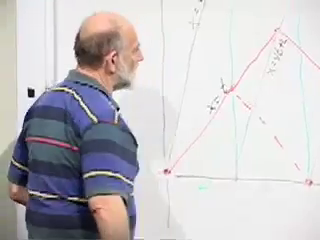
\includegraphics[width=0.72\textwidth]{lecture_01_figure_04.png}
\caption{Tia sáng truyền sang phải \(x=t\) cắt đường thế giới chuyển động ở giữa.}
\lectureframe{01:02:33}
\end{figure}

Có thể vẽ toàn bộ hình học mà không bị một người đứng trước bảng che khuất:

\begin{figure}[H]
\centering
\begin{tikzpicture}[scale=0.95]
\draw[->] (-0.5,0) -- (6.5,0) node[right] {$x$};
\draw[->] (0,-0.2) -- (0,4.3) node[above] {$t$};
\draw[blue] (0,0) -- (1.4,4.0);
\draw[blue] (2.0,0) -- (3.4,4.0);
\draw[blue] (4.0,0) -- (5.4,4.0);
\draw[red] (0,0) -- (3.08,3.08);
\draw[red] (3.08,3.08) -- (4.56,1.60);
\draw[red,dashed] (2.0,0) -- (4.56,1.60);
\fill (0,0) circle (1.5pt);
\fill (2.0,0) circle (1.5pt);
\fill (4.0,0) circle (1.5pt);
\fill (3.08,3.08) circle (1.5pt);
\fill (4.56,1.60) circle (1.5pt);
\node[left] at (0.55,1.55) {$x=vt$};
\node[left] at (2.45,1.9) {$x=vt+L$};
\node[right] at (4.72,1.9) {$x=vt+2L$};
\node[left] at (1.88,2.28) {$x=t$};
\node[above right] at (3.08,3.08) {$A$};
\end{tikzpicture}
\caption{Các tín hiệu ánh sáng xác định đường đồng thời của hệ quy chiếu chuyển động.}
\end{figure}

Cho một tia sáng truyền sang phải xuất phát từ gốc tọa độ. Gọi \(A\) là giao điểm của nó với đường thế giới ở giữa. Hai phương trình tại \(A\) là
\begin{align}
x&=t,\\
x&=vt+L.
\end{align}
Thế vào ta được
\begin{equation}
t=vt+L,
\end{equation}
và do đó
\begin{equation}
t_A=x_A=\frac{L}{1-v}.
\label{eq:point-a}
\end{equation}

Từ \(A\), lần ngược một tia sáng truyền sang trái tới đường thế giới chuyển động ngoài cùng bên phải. Phương trình của nó có dạng
\begin{equation}
x+t=b.
\end{equation}
Vì nó đi qua \(A\), Phương trình~\eqref{eq:point-a} xác định hằng số:
\begin{equation}
b=x_A+t_A=\frac{2L}{1-v}.
\end{equation}
Vì vậy tia đi ngược thỏa mãn
\begin{equation}
x+t=\frac{2L}{1-v}.
\label{eq:backward-ray}
\end{equation}

Giao điểm của nó với đường thế giới ngoài cùng bên phải được suy ra từ
\begin{align}
x+t&=\frac{2L}{1-v},\\
x&=vt+2L.
\end{align}
Loại \(x\) đi,
\begin{align}
(1+v)t
  &=2L\left(\frac{1}{1-v}-1\right)\\
  &=\frac{2Lv}{1-v},
\end{align}
nên
\begin{equation}
t=\frac{2Lv}{1-v^2}.
\end{equation}
Thế vào \(x=vt+2L\) cho
\begin{equation}
x=\frac{2L}{1-v^2}.
\end{equation}
Bản thân các tọa độ kém quan trọng hơn tỷ số của chúng:
\begin{equation}
\frac{t}{x}=v.
\end{equation}
Vì vậy mọi sự kiện đồng thời với gốc tọa độ theo các đồng hồ chuyển động đều nằm trên
\begin{equation}
t=vx,
\label{eq:simultaneity-c-one}
\end{equation}
trong khi gốc tọa độ chuyển động đi theo
\begin{equation}
x=vt.
\label{eq:moving-time-axis}
\end{equation}
Hai trục nghiêng đối xứng quanh tia sáng \(45^\circ\).

Mọi điểm trên \(x=vt\) đều có cùng vị trí có dấu phẩy, \(x'=0\), trong khi thời gian có dấu phẩy của chúng biến thiên. Mọi điểm trên \(t=vx\) đều có cùng thời gian có dấu phẩy, \(t'=0\), trong khi vị trí có dấu phẩy của chúng biến thiên. Vì thế một đường là trục thời gian có dấu phẩy và đường kia là trục không gian có dấu phẩy. Cần đến phép dựng tín hiệu dài dòng ấy để xác định đường thứ hai; không thể suy ra nó chỉ từ riêng đường thế giới chuyển động.

Khôi phục các đơn vị thông thường trong Phương trình~\eqref{eq:simultaneity-c-one} đòi hỏi
\begin{equation}
t=\frac{v}{c^2}x.
\label{eq:simultaneity-dimensional}
\end{equation}
Thừa số \(c^2\) giải thích vì sao bức tranh Newton hoạt động tốt đến vậy trong đời sống hằng ngày. Với các vận tốc rất nhỏ so với \(c\), độ dốc của đường đồng thời chuyển động là cực kỳ nhỏ.

\begin{figure}[H]
\centering
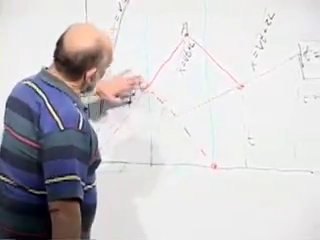
\includegraphics[width=0.72\textwidth]{lecture_01_figure_05.png}
\caption{Với \(c=1\), trục thời gian có dấu phẩy và trục đồng thời đối xứng nhau qua tia sáng.}
\lectureframe{01:15:40}
\end{figure}

\begin{figure}[H]
\centering
\begin{tikzpicture}[scale=1.0]
\draw[->] (-2.2,0) -- (5.2,0) node[right] {$x$};
\draw[->] (0,-0.2) -- (0,4.9) node[above] {$t$};
\draw[red] (0,0) -- (3.9,3.9);
\draw[red] (0,0) -- (-1.8,1.8);
\draw[blue] (0,0) -- (1.8,4.5);
\draw[blue,dashed] (0,0) -- (4.5,1.8);
\node[right] at (3.9,3.9) {$x=t$};
\node[left] at (-1.8,1.8) {$x=-t$};
\node[above] at (1.8,4.5) {$x'=0$};
\node[right] at (4.5,1.8) {$t'=0$};
\end{tikzpicture}
\caption{Các trục có dấu phẩy và các tia sáng bất biến khi dùng các đơn vị \(c=1\).}
\end{figure}

\section{Suy ra phép biến đổi Lorentz}

Hình học xác định nơi mỗi tọa độ có dấu phẩy triệt tiêu. Dọc theo trục thời gian chuyển động \(x=vt\), ta phải có \(x'=0\). Dọc theo trục đồng thời chuyển động \(t=vx\), ta phải có \(t'=0\). Các quan hệ tuyến tính tổng quát nhất có đúng những tập triệt tiêu đó có thể viết thành
\begin{align}
x'&=\frac{x-vt}{F(v)},\\
t'&=\frac{t-vx}{G(v)}.
\label{eq:fg-ansatz}
\end{align}
Các thừa số \(F\) và \(G\) cho phép thang đo của các tọa độ có dấu phẩy khác với các thang đo Galile dù các trục đã được xác định. Tính tuyến tính suy ra từ tính đồng nhất của không gian và thời gian: tịnh tiến một thí nghiệm không thể làm thay đổi quy luật biến đổi.\editorialnote{Lập luận ngắn gọn này về tính tuyến tính làm tường minh một giả thiết đã được dùng ngầm trong phép suy diễn trên bảng.}

Ở giai đoạn này, hình học đã cho ta biết rất nhiều nhưng chưa phải mọi thứ. Các tử số xác định độ nghiêng của các trục. Chúng không xác định khoảng cách đơn vị dọc theo các trục ấy. Chính phần thông tin về thang đo còn lại đó là điều mà \(F(v)\) và \(G(v)\) biểu diễn.

Bây giờ áp đặt tính bất biến của tốc độ ánh sáng. Một tia truyền sang phải thỏa \(x=t\) cũng phải thỏa \(x'=t'\). Dọc theo tia ấy,
\begin{align}
x'&=\frac{(1-v)t}{F(v)},\\
t'&=\frac{(1-v)t}{G(v)}.
\end{align}
Đẳng thức tại mọi điểm trên tia đòi hỏi
\begin{equation}
F(v)=G(v).
\end{equation}
Vì vậy ta có thể viết
\begin{align}
x'&=\frac{x-vt}{F(v)},\\
t'&=\frac{t-vx}{F(v)}.
\label{eq:common-f}
\end{align}

Bước này sử dụng đòi hỏi đầu tiên thật sự mang tính Einstein trong phần đại số. Cùng một đường hình học là một tia sáng đối với cả hai quan sát viên, nên hai tọa độ có dấu phẩy phải tăng như nhau dọc theo nó khi \(c=1\). Những thừa số khác nhau trong hai phương trình sẽ làm cho tốc độ có dấu phẩy khác 1.

Còn lại một hàm chưa biết. Nhân Phương trình~\eqref{eq:common-f} với \(F(v)\):
\begin{align}
F(v)x'&=x-vt,\\
F(v)t'&=t-vx.
\end{align}
Nhân phương trình thứ hai với \(v\) rồi cộng vào phương trình thứ nhất sẽ khử \(t\), ta được
\begin{equation}
(1-v^2)x=F(v)(x'+vt').
\end{equation}
Tương tự,
\begin{equation}
(1-v^2)t=F(v)(t'+vx').
\end{equation}
Vì thế phép biến đổi nghịch đảo là
\begin{align}
x&=\frac{F(v)}{1-v^2}(x'+vt'),\\
t&=\frac{F(v)}{1-v^2}(t'+vx').
\end{align}

Nguyên lý tương đối khiến hai hệ quy chiếu là tương hỗ. Nếu nhà ga thấy đoàn tàu chuyển động với \(+v\), thì đoàn tàu thấy nhà ga chuyển động với \(-v\). Do đó các phương trình nghịch đảo phải có cùng dạng với các phương trình thuận khi đổi dấu \(v\). Các hệ số đứng trước của chúng phải thỏa
\begin{equation}
\frac{F(v)}{1-v^2}=\frac{1}{F(v)}.
\end{equation}
Suy ra
\begin{equation}
F(v)^2=1-v^2,
\end{equation}
và tính liên tục với phép biến đổi đồng nhất tại \(v=0\) chọn nghiệm dương,
\begin{equation}
F(v)=\sqrt{1-v^2}.
\end{equation}

Không có gì ở đây được điều chỉnh để khớp với một xung ánh sáng cụ thể nào. Kết quả suy ra từ các trục được cố định bởi phép đồng bộ hóa, từ tốc độ chung của ánh sáng và từ yêu cầu rằng không hệ quy chiếu quán tính nào được ưu tiên hơn hệ kia.

Phép biến đổi Lorentz trong các đơn vị với \(c=1\) là
\begin{align}
x'&=\frac{x-vt}{\sqrt{1-v^2}},\\
t'&=\frac{t-vx}{\sqrt{1-v^2}}.
\label{eq:lorentz-c-one}
\end{align}
Nghịch đảo của nó là
\begin{align}
x&=\frac{x'+vt'}{\sqrt{1-v^2}},\\
t&=\frac{t'+vx'}{\sqrt{1-v^2}}.
\end{align}

\begin{figure}[H]
\centering
\includegraphics[width=0.76\textwidth]{lecture_01_figure_06.png}
\caption{Phép biến đổi Lorentz với \(c=1\) ở dạng hoàn chỉnh trên bảng.}
\lectureframe{01:32:38}
\end{figure}

Điểm mới cốt yếu đã hiện rõ ngay trong phương trình thời gian. Thời gian không đơn giản được chuyển nguyên vẹn từ hệ này sang hệ kia. Một tọa độ thời gian có dấu phẩy pha trộn thời gian và vị trí không dấu phẩy. Hệ quả là \(t=\text{constant}\) và \(t'=\text{constant}\) mô tả những tập sự kiện khác nhau.

Hạng trộn này không phải là một hiệu chỉnh tùy chọn được gắn thêm về sau. Không có nó, đường \(t'=0\) sẽ vẫn nằm ngang, tính đồng thời ở xa sẽ vẫn là phổ quát, và phép biến đổi sẽ không thể bảo toàn tốc độ ánh sáng.

\section{Khôi phục tốc độ ánh sáng và kiểm tra kết quả}

Khi \(c\ne1\), tính nhất quán thứ nguyên khôi phục các thừa số còn thiếu. Tỉ số \(v^2/c^2\) là vô thứ nguyên, còn \((v/c^2)x\) có đơn vị thời gian. Vì thế
\begin{align}
x'&=\frac{x-vt}{\sqrt{1-v^2/c^2}},\\
t'&=\frac{t-(v/c^2)x}{\sqrt{1-v^2/c^2}}.
\label{eq:lorentz-dimensional}
\end{align}
Nghịch đảo thu được bằng cách đổi dấu \(v\):
\begin{align}
x&=\frac{x'+vt'}{\sqrt{1-v^2/c^2}},\\
t&=\frac{t'+(v/c^2)x'}{\sqrt{1-v^2/c^2}}.
\end{align}
Việc đưa vào
\begin{equation}
\gamma=\frac{1}{\sqrt{1-v^2/c^2}}
\end{equation}
sẽ đưa chúng về dạng gọn quen thuộc, nhưng dạng viết qua mẫu số này giữ cho phép suy diễn vẫn hiện rõ.

Về mặt số trị, \(c\simeq3\times10^8\,\mathrm{m/s}\), nên \(c^2\simeq9\times10^{16}\,\mathrm{m^2/s^2}\). Mẫu số lớn làm cho cả độ nghiêng của đường đồng thời lẫn thừa số \(v^2/c^2\) đều không thể nhận thấy trong phần lớn các thí nghiệm cơ học. Sự nhỏ bé của chúng giải thích thành công của Galileo; nó không khôi phục thời gian tuyệt đối.

\begin{figure}[H]
\centering
\includegraphics[width=0.76\textwidth]{lecture_01_figure_07.png}
\caption{Phép biến đổi Lorentz sau khi đã khôi phục các thừa số \(c\).}
\lectureframe{01:35:58}
\end{figure}

Có thể kiểm tra ngay hai điều. Trước hết, xét \(v\ll c\). Khi đó \(v^2/c^2\) là không đáng kể, và với các khoảng cách thông thường thì số hạng \(vx/c^2\) biểu thị tính tương đối của sự đồng thời cũng không đáng kể. Phương trình~\eqref{eq:lorentz-dimensional} rút gọn thành
\begin{equation}
t'\approx t,\qquad x'\approx x-vt.
\end{equation}
Phép tương đối Galileo được khôi phục như gần đúng tốc độ thấp.

Thứ hai, hãy kiểm tra một tia sáng. Sau khi \(c\) đã được khôi phục, một tia truyền sang phải thỏa mãn \(x=ct\), không phải \(x=t\). Thế vào, ta được
\begin{align}
x'&=\frac{(c-v)t}{\sqrt{1-v^2/c^2}},\\
t'&=\frac{(1-v/c)t}{\sqrt{1-v^2/c^2}}.
\end{align}
Vì \(c-v=c(1-v/c)\),
\begin{equation}
x'=ct'.
\end{equation}
Người quan sát ở hệ phẩy đo được cùng tốc độ \(c\). Với một tia truyền sang trái, việc thay \(x=-ct\) vào tương tự cho
\begin{equation}
x'=-ct'.
\end{equation}
Phép biến đổi xử lý đúng ánh sáng truyền theo cả hai hướng.

Sự phân biệt giữa \(x=t\) và \(x=ct\) là một phép kiểm tra thứ nguyên rất bổ ích. Biểu thức thứ nhất chỉ đúng trong hệ đơn vị mà \(c=1\). Việc khôi phục các đơn vị thông thường trong phép biến đổi mà vẫn để phương trình tia ở đơn vị tự nhiên sẽ trộn lẫn hai quy ước và cho ra một kết quả sai. Tính nhất quán thứ nguyên phát hiện sai lầm đó ngay lập tức.

\section{Tiêu chuẩn trung điểm}

\begin{classroomqa}
\audiencequestion{Giả sử một người quan sát nhận được hai chớp sáng vào cùng một thời điểm nhưng không ở chính giữa hai nguồn phát của chúng. Người quan sát đó có thể kết luận rằng hai chớp sáng đã được phát ra đồng thời không?
\lecturetimestamp{01:42:55}}
\lecturerresponse{Không. Thời điểm đến bằng nhau chỉ kéo theo thời điểm phát bằng nhau đối với người quan sát nằm đúng tại trung điểm không gian giữa hai nguồn trong hệ quy chiếu thích hợp. Một máy thu ở gần một nguồn hơn vẫn có thể nhận đồng thời cả hai chớp sáng, mặc dù chớp sáng ở xa hơn đã được phát ra sớm hơn. Vì vậy, trong dựng hình chuyển động, đường thế giới trung điểm \(x=vt+L\) là thiết yếu. Tia đi sang phải \(x=t\) được theo dõi cho đến khi gặp trung điểm đó, rồi một tia sáng ngược chiều được lần theo tới \(x=vt+2L\). Biến cố đầu mút thứ hai ấy, chứ không phải một biến cố nhận đồng thời tùy ý ở nơi khác, mới đồng thời với gốc theo hệ quy chiếu chuyển động.}
\end{classroomqa}

Chúng ta đã đi tới phép biến đổi tọa độ đầy đủ, nhưng chưa tới những hệ quả quen thuộc nhất của nó. Tiếp theo sẽ là sự co độ dài, sự giãn thời gian và thời gian riêng, rồi đến động lượng và năng lượng tương đối tính. Nền tảng đã được đặt xong: mỗi hệ quy chiếu quán tính chỉ có thể dùng cùng các định luật và đo được cùng tốc độ ánh sáng bởi vì không gian và thời gian trộn lẫn với nhau, và bởi vì tính đồng thời của các sự kiện ở xa thuộc về một hệ quy chiếu chứ không phải thuộc về thế giới một cách tuyệt đối.

\chapter{Các phương trình Maxwell, tính hiệp biến và sóng điện từ}

\lectureoverview{Điện trường và từ trường tác dụng lên vật chất mang điện thông qua lực Lorentz, nhưng vật chất cũng phải tạo ra và sắp xếp lại các trường đó. Chúng ta sẽ phát biểu nửa đối ứng ấy của điện từ học, chỉ ra rằng các phương trình Maxwell là hiệp biến Lorentz, suy ra các nghiệm sóng của chúng, rồi đưa điện tích và dòng điện trở lại dưới một dạng làm cho sự bảo toàn địa phương trở nên tường minh. Trong suốt bài giảng, ta dùng hệ đơn vị trong đó \(c=1\).}

\section{Nửa kia của điện từ học}

Hãy bắt đầu với phần của chủ đề mà ta đã có trong tay. Nếu một hạt có điện tích \(q\) chuyển động với vận tốc \(\mathbf v\) qua điện trường và từ trường, thì lực là
\begin{equation}
\mathbf F=q\bigl(\mathbf E+\mathbf v\times\mathbf B\bigr).
\label{eq:lorentz-force-three}
\end{equation}
Thừa số \(q\) là không thể thiếu. Một hạt không mang điện không cảm nhận lực điện từ. Điện trường đóng góp ngay cả khi hạt tức thời đứng yên, còn đóng góp của từ trường thì phụ thuộc vào chuyển động của nó.

Phương trình~\eqref{eq:lorentz-force-three} cho ta biết các trường đã cho sẵn tác dụng lên vật chất như thế nào. Nó không cho ta biết điều gì quyết định các trường ấy. Điều gì tạo ra điện trường quanh một vật, từ trường quanh một vật khác, hay một sóng chuyển động qua không gian trống? Các phương trình trả lời những câu hỏi đó là các phương trình Maxwell.

\begin{figure}[H]
\centering
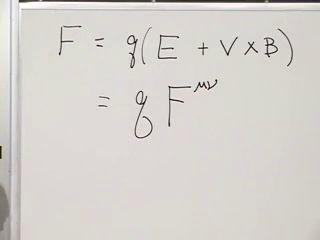
\includegraphics[width=0.62\textwidth]{lecture_58_figure_02.png}
\caption{Lực Lorentz dạng ba-vectơ và phần mở đầu của việc viết lại nó dưới dạng tensor.}
\lectureframe{00:05:49}
\end{figure}

Dạng tương đối tính của định luật lực báo trước ký hiệu mà ta sẽ cần:
\begin{equation}
f^\mu=qF^\mu{}_{\nu}u^\nu.
\label{eq:lorentz-force-four}
\end{equation}
Ở đây \(u^\nu\) là bốn-vận tốc, \(f^\mu\) là bốn-lực, và \(F^{\mu\nu}\) là một tensor phản đối xứng được ghép từ \(\mathbf E\) và \(\mathbf B\). Trên bảng lúc đầu chỉ hiển thị phần mở đầu sơ lược của biểu thức này; phép co với \(u^\nu\) cung cấp vectơ còn thiếu cần để còn lại một chỉ số lực tự do.

Có một lý do vật lý khiến vật chất phải tác dụng ngược trở lại lên trường. Một sóng điện từ có thể đập vào một điện tích, gia tốc nó và truyền năng lượng cho nó. Nếu trường có thể ảnh hưởng lên điện tích trong khi điện tích lại không bao giờ có thể ảnh hưởng lên trường, thì sẽ không có nơi nào mà năng lượng đó bị rút ra. Tác dụng và phản tác dụng chưa hẳn là toàn bộ lập luận, nhưng sự bảo toàn năng lượng khiến sự ghép đôi đối ứng ấy trở thành điều không thể tránh khỏi.

\section{Một nguồn biến thiên phát ra một nhiễu động}

Một điện tích điểm tạo ra một điện trường hướng ra ngoài hoặc vào trong tính từ vị trí của nó. Một dòng điện trong dây dẫn--một dòng các hạt mang điện--tạo ra một từ trường tuần hoàn quanh dây. Những hình ảnh tĩnh quen thuộc này đã cho thấy hai mẫu hình học khác nhau: thông lượng điện tỏa ra từ điện tích, còn các đường sức từ thì quấn quanh dòng điện.

Bây giờ hãy dịch chuyển điện tích điểm một cách đột ngột. Gần vị trí mới của nó, điện trường phải bắt đầu sắp xếp lại, nhưng một quan sát viên ở xa không thể biết được chuyển động ấy ngay tức thì. Trường cũ vẫn còn ở xa cho đến khi tín hiệu có đủ thời gian để tới nơi. Giữa vùng gần và vùng xa là một mặt lan truyền mà tại đó trường đang biến đổi. Sự sắp xếp lại đang chuyển động ấy là một nhiễu động điện từ.

Nếu điện tích bị cưỡng bức dao động qua lại, các sự sắp xếp lại kế tiếp nhau sẽ nối tiếp nhau và tạo thành một sóng điện từ. Đây là chức năng sơ đẳng của một ăng-ten: một dòng điện dao động phát nhiễu động trường ra ngoài. Đảo chiều một dòng điện trong dây cho phiên bản từ của cùng lập luận đó. Sự tuần hoàn của \(\mathbf B\) phải đảo chiều, nhưng sự đảo chiều ấy lan truyền đi thay vì xuất hiện đồng thời ở khắp nơi.

Bức tranh nhân quả này đặt ra hai mục tiêu cho các phương trình Maxwell. Chúng phải mô tả cách điện tích và dòng điện làm nguồn cho các trường, và chúng phải cho phép những biến đổi của các trường ấy lan truyền không nhanh hơn ánh sáng. Mục tiêu thứ hai đồng thời cũng là một phép kiểm tra của thuyết tương đối. Nếu các phương trình Maxwell có cùng dạng trong mọi hệ quy chiếu quán tính và hàm ý một tốc độ sóng xác định, thì mọi hệ quy chiếu quán tính đều phải suy ra cùng tốc độ đó từ chúng.

\section{Ôn lại phương trình sóng tương đối tính}

Trước khi chuyển sang các trường vectơ, hãy xét một trường vô hướng \(\phi(\mathbf x,t)\), một giá trị số tại mỗi điểm không-thời gian. Một phương trình đạo hàm bậc nhất
\begin{equation}
\partial_\mu\phi=0
\end{equation}
sẽ nói rằng mọi đạo hàm theo không-thời gian đều triệt tiêu. Khi đó trường sẽ là hằng số và vì vậy không thể mang một sóng. Một phương trình sóng tương đối tính không tầm thường dùng hai đạo hàm:
\begin{equation}
\partial_\mu\partial^\mu\phi=0.
\end{equation}
Với quy ước dấu dùng ở đây,
\begin{equation}
\left(\partial_t^2-\partial_x^2-\partial_y^2-\partial_z^2\right)\phi=0,
\label{eq:scalar-wave-four}
\end{equation}
hay, gọn hơn,
\begin{equation}
\left(\partial_t^2-\nabla^2\right)\phi=0.
\end{equation}
Lựa chọn \(c=1\) khiến thời gian và khoảng cách mang các đơn vị tương thích. Nếu khôi phục các đơn vị thông thường thì \(1/c^2\) sẽ đứng cạnh đạo hàm thời gian bậc hai.

Đối với một sóng truyền dọc theo trục \(z\), trường phụ thuộc vào \(z\) và \(t\), không phụ thuộc vào \(x\) hay \(y\). Phương trình~\eqref{eq:scalar-wave-four} rút gọn thành
\begin{equation}
\left(\partial_t^2-\partial_z^2\right)\phi=0.
\label{eq:scalar-wave-one}
\end{equation}

\begin{figure}[H]
\centering
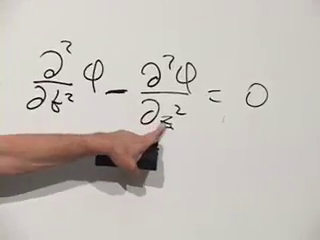
\includegraphics[width=0.56\textwidth]{lecture_58_figure_04.png}
\caption{Phương trình sóng vô hướng một chiều được dùng làm mô hình cho sóng điện từ.}
\lectureframe{00:47:03}
\end{figure}

Dạng sóng truyền tổng quát của nó là
\begin{equation}
\phi(z,t)=f(z-t)+g(z+t).
\end{equation}
Biên dạng \(f(z-t)\) chuyển động về phía \(z\) tăng, vì một điểm có pha cố định thỏa mãn \(z-t=\text{constant}\). Biên dạng \(g(z+t)\) chuyển động theo chiều ngược lại. Không có gì buộc một trong hai biên dạng phải là hình sin; bất kỳ dạng nào đủ trơn cũng tịnh tiến mà không đổi dạng.

Tuy vậy, các hàm sin vẫn thuận tiện:
\begin{equation}
\phi(z,t)=A\cos\!\bigl(k(z-t)\bigr).
\end{equation}
Số sóng \(k\) quyết định bước sóng,
\begin{equation}
\lambda=\frac{2\pi}{k}.
\end{equation}
\(k\) lớn tạo ra dao động không gian nhanh và bước sóng ngắn; \(k\) nhỏ tạo ra bước sóng dài. Những biên dạng này ngay sau đây sẽ trở thành các thành phần của \(\mathbf E\) và \(\mathbf B\).

\section{Giải tích vectơ mà Maxwell cần dùng}

Các phương trình Maxwell được viết bằng tích vô hướng, tích có hướng, độ phân kỳ và độ xoáy. Đáng để dựng lại hệ ký hiệu này một lần, vì các phép tính theo thành phần về sau dùng đúng chính những mẫu đó.

Đối với các ba-vectơ thông thường \(\mathbf a\) và \(\mathbf b\), tích vô hướng là vô hướng
\begin{equation}
\mathbf a\cdot\mathbf b
=a_xb_x+a_yb_y+a_zb_z.
\end{equation}
Tích có hướng là một vectơ khác,
\begin{align}
(\mathbf a\times\mathbf b)_x&=a_yb_z-a_zb_y,\\
(\mathbf a\times\mathbf b)_y&=a_zb_x-a_xb_z,\\
(\mathbf a\times\mathbf b)_z&=a_xb_y-a_yb_x.
\end{align}
Các thành phần còn lại tuân theo thứ tự tuần hoàn \(x\to y\to z\to x\).

Hãy đưa vào toán tử vi phân
\begin{equation}
\boldsymbol\nabla=
\left(\partial_x,\partial_y,\partial_z\right).
\end{equation}
Các phần tử của nó là các toán tử chứ không phải các số thông thường, nhưng vẫn có thể dùng các mẫu tích vô hướng và tích có hướng. Với một trường vectơ \(\mathbf A\),
\begin{equation}
\boldsymbol\nabla\cdot\mathbf A
=\partial_xA_x+\partial_yA_y+\partial_zA_z
\label{eq:divergence}
\end{equation}
là độ phân kỳ, còn
\begin{align}
(\boldsymbol\nabla\times\mathbf A)_x
 &=\partial_yA_z-\partial_zA_y,\\
(\boldsymbol\nabla\times\mathbf A)_y
 &=\partial_zA_x-\partial_xA_z,\\
(\boldsymbol\nabla\times\mathbf A)_z
 &=\partial_xA_y-\partial_yA_x
\label{eq:curl}
\end{align}
là các thành phần của độ xoáy.

Hình học cũng quan trọng như các công thức. Một trường vectơ có độ phân kỳ dương ở nơi nó có vẻ chảy ra ngoài từ một nguồn. Nó có độ xoáy ở nơi nó tuần hoàn. Điện trường hướng tâm của một điện tích điểm minh họa độ phân kỳ; từ trường quấn quanh một dây dẫn có dòng điện minh họa độ xoáy. Một trường vectơ không đổi theo không gian thì không có phân kỳ lẫn xoáy.

\section{Các phương trình Maxwell trong chân không}

Khi không có điện tích và dòng điện, các phương trình Maxwell là
\begin{align}
\boldsymbol\nabla\times\mathbf E&=-\partial_t\mathbf B,
\label{eq:faraday-vac}\\
\boldsymbol\nabla\cdot\mathbf B&=0,
\label{eq:gauss-b-vac}\\
\boldsymbol\nabla\times\mathbf B&=\partial_t\mathbf E,
\label{eq:ampere-vac}\\
\boldsymbol\nabla\cdot\mathbf E&=0.
\label{eq:gauss-e-vac}
\end{align}
Hai phương trình xoáy gần như hoán đổi \(\mathbf E\) và \(\mathbf B\), nhưng một dấu trừ thiết yếu phân biệt chúng. Hai phương trình phân kỳ nói rằng cả hai trường đều không có nguồn trong miền chân không đang xét. Độ phân kỳ từ vẫn bằng không ngay cả sau khi khôi phục các nguồn điện; điện từ học thông thường không có điện tích từ.

\begin{figure}[H]
\centering
\includegraphics[width=0.76\textwidth]{lecture_58_figure_06.png}
\caption{Bốn phương trình Maxwell trong chân không, được sắp xếp để bộc lộ tính đối xứng gần đúng giữa điện trường và từ trường.}
\lectureframe{00:27:30}
\end{figure}

Mật độ điện tích \(\rho\) rốt cuộc sẽ thay số 0 ở vế phải của Phương trình~\eqref{eq:gauss-e-vac}, và mật độ dòng điện \(\mathbf J\) sẽ đi vào Phương trình~\eqref{eq:ampere-vac}. Tạm thời ta hoãn các hạng đó lại. Các phương trình không nguồn bộc lộ cấu trúc biến đổi và cơ chế sóng với mức rườm rà ít nhất.

Chúng cũng làm sắc nét nghịch đề của Einstein. Một quan sát viên Galile đi theo một sóng sẽ mong đợi trừ các vận tốc và đo được một tốc độ sóng nhỏ hơn. Thế nhưng nếu cùng các phương trình Maxwell đúng trong mọi hệ quy chiếu quán tính, thì mỗi quan sát viên đều suy ra cùng một tốc độ sóng đơn vị. Lối thoát không phải là thay đổi phương trình sóng từ hệ này sang hệ khác. Mà là dùng phép biến đổi Lorentz và biểu diễn các phương trình Maxwell bằng những đối tượng mà các quy luật biến đổi của chúng đã được biết sẵn.

\section{Điện trường và từ trường trong một tensor duy nhất}

Điện trường và từ trường kết hợp thành tensor trường phản đối xứng
\begin{equation}
F^{\mu\nu}=
\begin{pmatrix}
0   & -E_x & -E_y & -E_z\\
E_x & 0    & -B_z & B_y\\
E_y & B_z  & 0    & -B_x\\
E_z & -B_y & B_x  & 0
\end{pmatrix},
\label{eq:l0203-field-tensor}
\end{equation}
trong đó thứ tự hàng và cột là \(t,x,y,z\). Tính phản đối xứng,
\begin{equation}
F^{\mu\nu}=-F^{\nu\mu},
\end{equation}
buộc các phần tử trên đường chéo phải triệt tiêu và xác định nửa dưới của ma trận từ nửa trên. Các phần tử thời gian-không gian chứa \(\mathbf E\); các phần tử thuần không gian chứa \(\mathbf B\).

\begin{figure}[H]
\centering
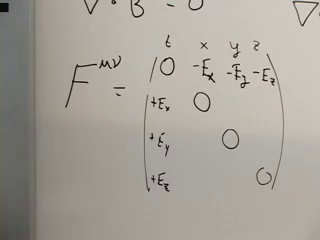
\includegraphics[width=0.58\textwidth]{lecture_58_figure_03.png}
\caption{Tensor trường điện từ hoàn chỉnh, bao gồm các phần tử điện và từ của nó.}
\lectureframe{00:32:05}
\end{figure}

Tầm quan trọng của \(F^{\mu\nu}\) không chỉ là việc sáu thành phần trường vừa khít trong một ma trận. Dưới một phép biến đổi Lorentz, nó biến đổi như một tensor hạng hai. Vì thế điện trường và từ trường do các quan sát viên khác nhau đo được trộn lẫn đúng theo cách cần thiết để toàn bộ đối tượng biến đổi một cách nhất quán.

Có một tensor phản đối xứng thứ hai, tensor trường đối ngẫu \(\widetilde F^{\mu\nu}\). Với quy ước hiện tại, nó thu được từ Phương trình~\eqref{eq:l0203-field-tensor} qua phép thay thế
\begin{equation}
\mathbf E\longmapsto-\mathbf B,
\qquad
\mathbf B\longmapsto\mathbf E.
\label{eq:dual-replacement}
\end{equation}
Do đó
\begin{equation}
\widetilde F^{\mu\nu}=
\begin{pmatrix}
0    & B_x  & B_y  & B_z\\
-B_x & 0    & -E_z & E_y\\
-B_y & E_z  & 0    & -E_x\\
-B_z & -E_y & E_x  & 0
\end{pmatrix}.
\label{eq:dual-tensor}
\end{equation}
Dấu trong Phương trình~\eqref{eq:dual-replacement} là quan trọng. Bài giảng trước hết thử phát biểu phép hoán đổi ấy bằng lời, nhận ra sự không khớp về dấu, rồi sửa lại trước khi hoàn tất ma trận.

\begin{figure}[H]
\centering
\includegraphics[width=0.58\textwidth]{lecture_58_figure_07.png}
\caption{Tensor đối ngẫu đang được dựng bằng cách hoán đổi các phần tử điện và từ với dấu thích hợp.}
\lectureframe{00:35:45}
\end{figure}

\section{Các phương trình chân không hiệp biến}

Mỗi phương trình Maxwell chứa một đạo hàm. Bắt đầu từ một tensor hạng hai và co một chỉ số đạo hàm thì còn lại một chỉ số tự do, nên các ứng viên hiệp biến tự nhiên là
\begin{align}
\partial_\mu F^{\mu\nu}&=0,
\label{eq:maxwell-covariant-vac}\\
\partial_\mu\widetilde F^{\mu\nu}&=0.
\label{eq:maxwell-dual-vac}
\end{align}
Với mỗi giá trị cố định của \(\nu\), Phương trình~\eqref{eq:maxwell-covariant-vac} là một phương trình. Vì \(\nu\) có thể là \(t,x,y,z\), nó gộp bốn phương trình vô hướng. Phương trình~\eqref{eq:maxwell-dual-vac} gộp bốn phương trình còn lại. Điều này khớp với hai phương trình vectơ về độ xoáy và hai phương trình vô hướng về độ phân kỳ trong danh sách ban đầu.

Ký hiệu gọn chỉ hữu ích nếu nó tái tạo được các phương trình quen thuộc. Lấy \(\nu=z\):
\begin{align}
\partial_\mu F^{\mu z}
&=\partial_tF^{tz}
  +\partial_xF^{xz}
  +\partial_yF^{yz}
  +\partial_zF^{zz}\\
&=-\partial_tE_z+\partial_xB_y-\partial_yB_x\\
&=-\partial_tE_z+
  \bigl(\boldsymbol\nabla\times\mathbf B\bigr)_z.
\end{align}
Hạng \(F^{zz}\) triệt tiêu do tính phản đối xứng. Cho kết quả bằng không thì ta được thành phần \(z\) của
\begin{equation}
\boldsymbol\nabla\times\mathbf B=\partial_t\mathbf E.
\end{equation}
Các thành phần \(x\) và \(y\) suy ra bằng cách quay vòng các chỉ số.

\begin{figure}[H]
\centering
\includegraphics[width=0.76\textwidth]{lecture_58_figure_08.png}
\caption{Khai triển theo thành phần của phương trình trường hiệp biến; phần tử tensor trên đường chéo triệt tiêu và các hạng còn lại tái dựng các phương trình Maxwell.}
\lectureframe{00:43:30}
\end{figure}

Bây giờ lấy thành phần thời gian:
\begin{align}
\partial_\mu F^{\mu t}
&=\partial_tF^{tt}
  +\partial_xF^{xt}
  +\partial_yF^{yt}
  +\partial_zF^{zt}\\
&=\partial_xE_x+\partial_yE_y+\partial_zE_z\\
&=\boldsymbol\nabla\cdot\mathbf E.
\end{align}
Vì vậy nó cho Phương trình~\eqref{eq:gauss-e-vac}. Thực hiện cùng những phép kiểm tra đó trên tensor đối ngẫu cho ra
\(\boldsymbol\nabla\cdot\mathbf B=0\) và
\(\boldsymbol\nabla\times\mathbf E=-\partial_t\mathbf B\).

Giờ đây các phương trình gọn đã được thiết lập chứ không còn chỉ là phỏng đoán. Cấu trúc chỉ số tự do của chúng khiến chúng là các phương trình bốn-vectơ, nên một phép biến đổi Lorentz làm thay đổi các thành phần của chúng nhưng không làm thay đổi dạng của chúng. Đây là nghĩa chính xác mà theo đó các phương trình Maxwell trong chân không là như nhau trong mọi hệ quy chiếu quán tính.

\section{Từ các phương trình bậc nhất đến một sóng}

Các phương trình Maxwell chỉ chứa các đạo hàm bậc nhất, trong khi một phương trình sóng chứa các đạo hàm bậc hai. Sự không khớp bề ngoài này được giải quyết vì lý thuyết Maxwell ghép cặp hai trường. Một cặp phương trình bậc nhất cho \(\mathbf E\) và \(\mathbf B\) có thể được kết hợp thành một phương trình bậc hai chỉ cho riêng một trong hai trường.

Lấy đạo hàm theo thời gian của Phương trình~\eqref{eq:ampere-vac}:
\begin{equation}
\partial_t^2\mathbf E
=\boldsymbol\nabla\times\partial_t\mathbf B.
\end{equation}
Định luật Faraday cung cấp đạo hàm theo thời gian của \(\mathbf B\),
\begin{equation}
\partial_t\mathbf B=-\boldsymbol\nabla\times\mathbf E,
\end{equation}
và do đó
\begin{equation}
\partial_t^2\mathbf E
=-\boldsymbol\nabla\times
  \bigl(\boldsymbol\nabla\times\mathbf E\bigr).
\label{eq:double-curl}
\end{equation}

Trên bảng người ta triển khai một thành phần thay vì viện dẫn một đồng nhất thức đã học thuộc. Với thành phần \(x\),
\begin{align}
\bigl[\boldsymbol\nabla\times
(\boldsymbol\nabla\times\mathbf E)\bigr]_x
&=\partial_y(\boldsymbol\nabla\times\mathbf E)_z
 -\partial_z(\boldsymbol\nabla\times\mathbf E)_y\\
&=\partial_y(\partial_xE_y-\partial_yE_x)\\
&\quad-\partial_z(\partial_zE_x-\partial_xE_z)\\
&=\partial_x(\partial_yE_y+\partial_zE_z)
 -\partial_y^2E_x\\
&\quad-\partial_z^2E_x.
\end{align}
Cộng rồi trừ \(\partial_x^2E_x\) để làm lộ ra độ phân kỳ:
\begin{align}
\bigl[\boldsymbol\nabla\times
(\boldsymbol\nabla\times\mathbf E)\bigr]_x
&=\partial_x(\boldsymbol\nabla\cdot\mathbf E)
 -\nabla^2E_x.
\label{eq:double-curl-x}
\end{align}
Trong chân không \(\boldsymbol\nabla\cdot\mathbf E=0\). Kết hợp
Phương trình~\eqref{eq:double-curl} và \eqref{eq:double-curl-x} cho
\begin{equation}
\left(\partial_t^2-\nabla^2\right)E_x=0.
\label{eq:ex-wave}
\end{equation}

\begin{figure}[H]
\centering
\includegraphics[width=0.72\textwidth]{lecture_58_figure_09.png}
\caption{Phép tính theo thành phần đi tới phương trình sóng cho \(E_x\).}
\lectureframe{00:57:10}
\end{figure}

Phép tính tương tự cũng áp dụng cho \(E_y\) và \(E_z\), và một phép khử tương tự cho ta
\begin{equation}
\left(\partial_t^2-\nabla^2\right)\mathbf B=0.
\end{equation}
Vì vậy, điện trường và từ trường có thể lan truyền trong không gian trống dưới dạng sóng. Trong hệ đơn vị dùng ở đây, tốc độ của chúng bằng một, nghĩa là tốc độ ấy là \(c\) khi khôi phục các đơn vị thông thường.

\section{Một sóng phẳng và sự phân cực của nó}

Xây dựng một sóng đơn giản truyền theo chiều dương của \(z\):
\begin{equation}
\mathbf E(z,t)
=\widehat{\mathbf x}\,E_0
  \cos\!\bigl(k(z-t)\bigr).
\label{eq:plane-e}
\end{equation}
Biên dạng của nó tịnh tiến dọc theo \(z\) mà không đổi dạng. Vì điện trường hướng theo trục \(x\), nên sóng được phân cực thẳng theo phương \(x\). Ta chọn \(E_y=0\) chỉ để giữ cho ví dụ đơn giản; cũng có thể đưa vào một phân cực ngang thứ hai.

Thành phần dọc không tự do theo cùng cách. Vì sóng chỉ phụ thuộc vào \(z\) và \(t\),
\begin{equation}
\boldsymbol\nabla\cdot\mathbf E
=\partial_zE_z=0.
\end{equation}
Do đó \(E_z\) có thể là một hằng số, nhưng nó không thể chứa biên dạng sóng biến thiên. Một trường nền đồng đều có thể được chồng thêm vào hoặc bỏ đi một cách độc lập; nó không phải là một phần của bức xạ đang lan truyền. Bản thân sóng là ngang:
\begin{equation}
\mathbf E_{\mathrm{wave}}\cdot\widehat{\mathbf z}=0.
\end{equation}

Định luật Faraday xác định từ trường. Đối với Phương trình~\eqref{eq:plane-e}, thành phần khác không duy nhất của \(\boldsymbol\nabla\times\mathbf E\) là thành phần \(y\),
\begin{equation}
(\boldsymbol\nabla\times\mathbf E)_y=\partial_zE_x.
\end{equation}
Do đó \(\partial_t\mathbf B\) hướng theo \(y\), và một lựa chọn tương thích là
\begin{equation}
\mathbf B(z,t)
=\widehat{\mathbf y}\,E_0
  \cos\!\bigl(k(z-t)\bigr).
\label{eq:plane-b}
\end{equation}
Trong hệ đơn vị này, biên độ điện trường và từ trường bằng nhau. Hướng của chúng tuân theo
\begin{equation}
\mathbf E\perp\mathbf B,
\qquad
\mathbf E\perp\widehat{\mathbf z},
\qquad
\mathbf B\perp\widehat{\mathbf z},
\qquad
\mathbf E\times\mathbf B\parallel\widehat{\mathbf z}.
\end{equation}

\begin{figure}[H]
\centering
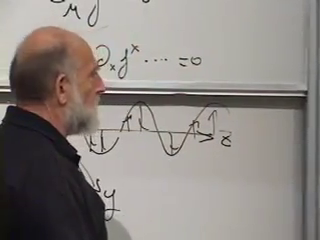
\includegraphics[width=0.70\textwidth]{lecture_58_figure_05.png}
\caption{Hình phác hoàn chỉnh trên bảng của một sóng điện từ ngang: các dao động của điện trường và từ trường vuông góc với nhau và với phương truyền.}
\lectureframe{01:05:25}
\end{figure}

\begin{figure}[H]
\centering
\scalebox{0.90}{%
\begin{tikzpicture}[x=1cm,y=1cm,>=Latex]
  \draw[->,thick] (0,0) -- (8.2,0) node[right] {$z$};
  \draw[->,thick] (0,-1.6) -- (0,1.7) node[above] {$x$};
  \draw[->,thick] (0,0) -- (-1.15,-0.8) node[below left] {$y$};
  \draw[blue!70!black,thick,domain=0:7.5,samples=120]
    plot (\x,{0.95*sin(90*\x)});
  \foreach \z/\s in {0.8/1,2.8/-1,4.8/1,6.8/-1}{
    \draw[->,green!45!black,thick]
      (\z,0) -- ++({-0.55*\s},{-0.38*\s});
  }
  \node[blue!70!black] at (6.9,1.25) {$\mathbf E$};
  \node[green!45!black] at (5.2,-1.05) {$\mathbf B$};
  \draw[->,very thick] (6.2,1.55) -- (7.7,1.55)
    node[midway,above] {propagation};
\end{tikzpicture}
}
\caption{Các trường \(\mathbf E\) và \(\mathbf B\) vuông góc với nhau và với phương truyền.}
\end{figure}

Đó là bản chất của ánh sáng và của mọi bức xạ điện từ trong chân không. Vì các phương trình đã sinh ra sóng này là hiệp biến Lorentz, nên một quan sát viên quán tính khác vẫn sẽ mô tả một sóng điện từ lan truyền với tốc độ \(c\), với điện trường và từ trường ngang.

\section{Mật độ điện tích và mật độ dòng điện}

Bây giờ ta khôi phục các nguồn đã tạm thời gác sang một bên. Khi nhiều hạt mang điện chiếm một vùng, sẽ hữu ích nếu thô hạt hóa chúng thành một mật độ điện tích liên tục
\begin{equation}
\rho(\mathbf x,t)=\frac{dQ}{dV}.
\end{equation}
Phép gần đúng này giống như việc coi nước là một chất lưu liên tục mặc dù nó được tạo thành từ các phân tử. Các điện tích dương và âm đóng góp với dấu ngược nhau, nên \(\rho\) là điện tích thuần trên một đơn vị thể tích.

Điện tích trong một vùng \(V\) được chọn là
\begin{equation}
Q_V(t)=\int_V\rho(\mathbf x,t)\,dV.
\label{eq:charge-volume}
\end{equation}
Mật độ ấy có thể biến thiên theo vị trí và thời gian. Một khối điện tích có thể rời khỏi một điểm, làm thay đổi mật độ cục bộ ở đó. Tuy nhiên, nó không thể biến thiên một cách tùy ý. Trong tự nhiên, điện tích được bảo toàn.

Chỉ bảo toàn toàn cục thôi thì còn quá yếu. Nó sẽ cho phép điện tích biến mất khỏi Trái Đất và đồng thời xuất hiện lại trên Sao Hỏa trong khi tổng điện tích vẫn không đổi. Phát biểu mạnh hơn là phát biểu cục bộ: điện tích chỉ có thể rời khỏi một nơi và đến một nơi khác thông qua một dòng chảy trong khoảng không gian xen giữa.

Để mô tả dòng chảy đó, hãy lấy một phần tử diện tích có hướng vi phân
\begin{equation}
d\boldsymbol\sigma=\widehat{\mathbf n}\,d\sigma.
\end{equation}
Độ lớn của nó là diện tích, còn hướng của nó là pháp tuyến với bề mặt. Mật độ dòng điện \(\mathbf J\) được định nghĩa sao cho điện tích đi qua phần tử ấy trong một đơn vị thời gian là
\begin{equation}
\frac{dQ}{dt}=\mathbf J\cdot d\boldsymbol\sigma.
\label{eq:current-flux-element}
\end{equation}
Độ lớn của \(\mathbf J\) là điện tích trên một đơn vị diện tích trong một đơn vị thời gian, còn hướng của nó là hướng dòng chảy của điện tích dương.

\begin{figure}[H]
\centering
\includegraphics[width=0.64\textwidth]{lecture_58_figure_10.png}
\caption{Một phần tử diện tích có hướng và thừa số thông lượng \(d\boldsymbol\sigma\cdot\mathbf J\).}
\lectureframe{01:18:15}
\end{figure}

Tích vô hướng chọn ra thành phần pháp tuyến với bề mặt. Một dòng điện tiếp tuyến với bề mặt không đi qua phía nào cả và đóng góp bằng không. Với độ lớn cố định, một dòng điện song song với pháp tuyến cho thông lượng lớn nhất. Dòng điện trong dây là một trường hợp đặc biệt, nhưng \(\mathbf J\) cũng có thể mô tả điện tích chảy qua một tấm hoặc khắp không gian ba chiều.

\section{Bảo toàn cục bộ và phương trình liên tục}

Giữ cố định một vùng \(V\) trong không gian và cho mọi phần tử trên biên kín \(\partial V\) của nó hướng ra ngoài. Nếu có dòng điện thuần hướng ra ngoài, thì điện tích bên trong giảm:
\begin{equation}
\frac{dQ_V}{dt}
=-\oint_{\partial V}\mathbf J\cdot d\boldsymbol\sigma.
\label{eq:integral-conservation}
\end{equation}
Dấu trừ là vật lý chứ không phải quy ước: thông lượng dương hướng ra ngoài lấy điện tích dương ra khỏi vùng ấy. Dùng Phương trình~\eqref{eq:charge-volume},
\begin{equation}
\int_V\partial_t\rho\,dV
=-\oint_{\partial V}\mathbf J\cdot d\boldsymbol\sigma.
\label{eq:integral-continuity-one}
\end{equation}

\begin{figure}[H]
\centering
\includegraphics[width=0.72\textwidth]{lecture_58_figure_11.png}
\caption{Định luật bảo toàn cho một vùng cố định sau khi thông lượng qua mặt được chuyển thành một phát biểu theo thể tích.}
\lectureframe{01:29:00}
\end{figure}

Định lý Gauss, còn gọi là định lý phân kỳ, liên hệ thông lượng qua một mặt kín với phân kỳ trong phần bên trong của nó:
\begin{equation}
\oint_{\partial V}\mathbf A\cdot d\boldsymbol\sigma
=\int_V\boldsymbol\nabla\cdot\mathbf A\,dV.
\label{eq:divergence-theorem}
\end{equation}
Ta có thể hình dung những ống ẩn bơm nước vào tại các điểm bên trong một bình chứa. Phân kỳ đo tốc độ cục bộ mà tại đó nước đi ra khỏi các đầu ống; tích phân mặt đo tổng lượng nước rời khỏi bình. Bất cứ thứ gì được tạo ra dưới dạng dòng chảy hướng ra ngoài ở bên trong cuối cùng cũng phải đi qua biên.

Áp dụng Phương trình~\eqref{eq:divergence-theorem} cho \(\mathbf J\) ta được
\begin{equation}
\int_V
\left(\partial_t\rho+\boldsymbol\nabla\cdot\mathbf J\right)dV=0.
\end{equation}
Hệ thức này đúng với mọi vùng \(V\) có thể chọn. Vì vậy, hàm dưới dấu tích phân phải triệt tiêu tại từng điểm:
\begin{equation}
\boxed{\partial_t\rho+\boldsymbol\nabla\cdot\mathbf J=0.}
\label{eq:continuity-three}
\end{equation}

\begin{figure}[H]
\centering
\includegraphics[width=0.72\textwidth]{lecture_58_figure_12.png}
\caption{Phương trình liên tục cục bộ được viết theo từng thành phần.}
\lectureframe{01:29:50}
\end{figure}

Phương trình~\eqref{eq:continuity-three} phát biểu đúng chính điều mà bảo toàn cục bộ đòi hỏi. Nếu mật độ điện tích giảm tại một điểm hoặc trong một vùng nhỏ, thì dòng điện phải phân kỳ ra ngoài từ đó. Nếu dòng điện hội tụ vào trong, mật độ điện tích tăng lên.

Mật độ và dòng điện kết hợp một cách tự nhiên thành bốn-dòng điện
\begin{equation}
J^\mu=(\rho,J_x,J_y,J_z)
\label{eq:four-current}
\end{equation}
trong hệ đơn vị \(c=1\). Phương trình liên tục trở thành phương trình vô hướng Lorentz
\begin{equation}
\partial_\mu J^\mu=0.
\label{eq:continuity-four}
\end{equation}
Dòng chảy của một phân bố tương đối tính phải biến đổi như một bốn-vectơ, cũng như bốn-vận tốc của một hạt đơn lẻ. Phương trình~\eqref{eq:continuity-four} làm cho bảo toàn điện tích cục bộ có hiệu lực trong mọi hệ quy chiếu quán tính.

\section{Các phương trình Maxwell có nguồn}

Khôi phục điện tích và dòng điện thì ta có
\begin{align}
\boldsymbol\nabla\cdot\mathbf E&=\rho,
\label{eq:gauss-e-source}\\
\boldsymbol\nabla\cdot\mathbf B&=0,\\
\boldsymbol\nabla\times\mathbf E&=-\partial_t\mathbf B,\\
\boldsymbol\nabla\times\mathbf B&=\partial_t\mathbf E+\mathbf J.
\label{eq:ampere-source}
\end{align}
Các phương trình có chứa nguồn điện gộp lại thành
\begin{equation}
\boxed{\partial_\mu F^{\mu\nu}=J^\nu,}
\label{eq:maxwell-source-covariant}
\end{equation}
trong khi cặp phương trình từ không nguồn vẫn là
\begin{equation}
\boxed{\partial_\mu\widetilde F^{\mu\nu}=0.}
\label{eq:maxwell-dual-source}
\end{equation}

\begin{figure}[H]
\centering
\includegraphics[width=0.78\textwidth]{lecture_58_figure_13.png}
\caption{Các phương trình Maxwell có nguồn đặt bên cạnh dạng hiệp biến của chúng \(\partial_\mu F^{\mu\nu}=J^\nu\).}
\lectureframe{01:34:00}
\end{figure}

Thành phần thời gian của Phương trình~\eqref{eq:maxwell-source-covariant} là
\begin{equation}
\partial_\mu F^{\mu t}=J^t=\rho,
\end{equation}
và phép tính theo thành phần đã thực hiện trước đó biến vế trái của nó thành
\(\boldsymbol\nabla\cdot\mathbf E\). Ba thành phần không gian cho lại
\(\boldsymbol\nabla\times\mathbf B=\partial_t\mathbf E+\mathbf J\).

Cũng có một phép kiểm tra tính nhất quán hữu ích. Cho \(\partial_\nu\) tác dụng lên
Phương trình~\eqref{eq:maxwell-source-covariant} thì được
\begin{equation}
\partial_\nu J^\nu
=\partial_\nu\partial_\mu F^{\mu\nu}=0,
\end{equation}
vì hai đạo hàm là đối xứng dưới \(\mu\leftrightarrow\nu\), còn \(F^{\mu\nu}\) thì phản đối xứng.\editorialnote{Phép kiểm tra ngắn gọn về tính nhất quán này suy ra từ phương trình hiệp biến và làm rõ vì sao các phương trình Maxwell có nguồn tự động tuân theo phương trình liên tục.}

Cấu trúc tương hỗ giờ đây đã hoàn chỉnh. Định luật lực tensor \(f^\mu=qF^\mu{}_\nu u^\nu\) mô tả cách các trường tác dụng lên điện tích, còn Phương trình~\eqref{eq:maxwell-source-covariant} mô tả cách điện tích và dòng điện sinh ra các trường. Cả hai đều là các phương trình tensor. Trong chân không, chính các phương trình trường ấy cho ra các sóng ngang lan truyền với tốc độ \(c\). Vì vậy, hiệp biến Lorentz và phương trình sóng điện từ gặp nhau đúng tại điểm đã thúc đẩy việc xây dựng này: mọi quan sát viên quán tính đều thu được cùng những định luật điện từ học và cùng một tốc độ ánh sáng.
\chapter{Thời gian riêng, sự giãn thời gian và sự co độ dài}

Chúng ta sẽ thường chọn hệ đơn vị trong đó tốc độ ánh sáng là $c=1$. Trong các đơn vị đó, một năm thời gian và một năm ánh sáng khoảng cách có thể được so sánh trực tiếp, và các công thức dễ đọc hơn nhiều. Bất cứ khi nào $c$ có ý nghĩa vật lý, ta sẽ đưa nó trở lại. Phân tích thứ nguyên là đủ để xác định chỗ cần đặt nó.

\section{Lưới không-thời gian Galile}

Hãy bắt đầu với hệ thức tiền Einstein giữa một hệ quy chiếu đứng yên và một đoàn tàu chuyển động với vận tốc $v$ dọc theo trục $x$:
\begin{align}
x' &= x-vt, & t'&=t.
\label{eq:l4-galilean}
\end{align}
Phương trình thứ hai chứa giả thiết thời gian tuyệt đối của Newton. Mọi quan sát viên đều dùng cùng các lát cắt đồng thời, dù các gốc tọa độ không gian chuyển động tương đối với nhau.

Giả sử quan sát viên không dấu phẩy đứng bên đường ray còn quan sát viên có dấu phẩy ngồi trên tàu. Gốc tọa độ của tàu có $x'=0$, nên đường thế giới của nó trong các tọa độ không dấu phẩy là
\begin{equation}
x=vt.
\end{equation}
Đường nghiêng đó là trục $t'$. Trái lại, $t'=t$ nói rằng mọi đường có $t'$ không đổi đều chính là những đường ngang như các đường có $t$ không đổi.

\begin{figure}[H]
\centering
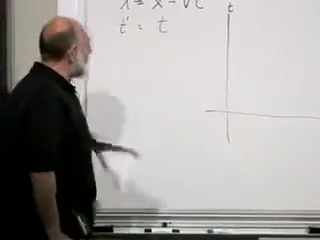
\includegraphics[width=0.72\textwidth]{lecture_04_figure_02.png}
\caption{Phép biến đổi Galile và lưới $t$-$x$ ban đầu. Gốc chuyển động sẽ vạch ra $x=vt$, trong khi hai hệ vẫn giữ chung các đường thời gian không đổi.}
\lectureframe{00:03:06}
\end{figure}

Giải phương trình~\eqref{eq:l4-galilean} theo các tọa độ không dấu phẩy, ta được
\begin{align}
x&=x'+vt'=x'+vt, & t&=t'.
\end{align}
Phép biến đổi nghịch đảo có cùng dạng, với $v$ được thay bằng $-v$. Nếu tàu chuyển động về phía trước so với ga, thì ga chuyển động lùi về phía sau so với tàu. Tính tương hỗ này vẫn còn trong thuyết tương đối hẹp, nhưng thời gian tuyệt đối thì không.

\section{Hiệu chỉnh Lorentz}

Các phép biến đổi Galile không thể làm cho tốc độ ánh sáng là như nhau trong mọi hệ quy chiếu quán tính. Các hệ thức đã hiệu chỉnh là, trước hết trong đơn vị $c=1$,
\begin{align}
x'&=\frac{x-vt}{\sqrt{1-v^2}}, &
t'&=\frac{t-vx}{\sqrt{1-v^2}}.
\label{eq:l4-lorentz-natural}
\end{align}
Khôi phục các đơn vị thông thường, ta được
\begin{align}
x'&=\frac{x-vt}{\sqrt{1-v^2/c^2}}, &
t'&=\frac{t-vx/c^2}{\sqrt{1-v^2/c^2}}.
\label{eq:l4-lorentz-c}
\end{align}

\begin{figure}[H]
\centering
\includegraphics[width=0.74\textwidth]{lecture_04_figure_05.png}
\caption{Phép biến đổi Lorentz với các thừa số $c$ được khôi phục.}
\lectureframe{00:09:10}
\end{figure}

Với $v\ll c$, cả $v^2/c^2$ lẫn $vx/c^2$ đều rất nhỏ trong những hoàn cảnh mà cơ học Newton được sử dụng. Khi đó, phương trình~\eqref{eq:l4-lorentz-c} quy về kết quả Galile. Thuyết tương đối không loại bỏ động học Newton; nó xác định miền hiệu lực của nó.

Tại $v=c$, mẫu số bằng không. Một hệ quy chiếu quán tính không thể chuyển động với tốc độ ánh sáng tương đối so với một hệ quy chiếu quán tính khác. Ở rất dưới giới hạn đó, các hiệu chỉnh là nhỏ, nhưng gần nó thì sự trộn lẫn giữa $x$ và $t$ trở nên không thể tránh khỏi.

Chuyển động đã được chọn dọc theo $x$, nên các tọa độ ngang không thay đổi:
\begin{equation}
y'=y,\qquad z'=z.
\end{equation}
Một cách để thấy vì sao là đặt các thước mét đặt ngang giống hệt nhau trên tàu và trên sân ga. Một quan sát viên chuyển động ở giữa hai hệ sẽ thấy các thanh tiến lại gần với những tốc độ bằng nhau và ngược chiều nhau. Cách bố trí này không có đặc điểm nào có thể khiến một thanh ngang ngắn hơn thanh kia.

\section{Các phép biến đổi Lorentz dọc theo nón ánh sáng}

Có một cách hình học để đọc phương trình~\eqref{eq:l4-lorentz-natural}. Cộng hai phương trình của nó:
\begin{align}
t'+x'
&=\frac{(t-vx)+(x-vt)}{\sqrt{1-v^2}}\\
&=(t+x)\frac{1-v}{\sqrt{1-v^2}}\\
&=(t+x)\sqrt{\frac{1-v}{1+v}}.
\label{eq:l4-null-plus}
\end{align}
Trừ chúng theo thứ tự còn lại:
\begin{align}
t'-x'
&=\frac{(t-vx)-(x-vt)}{\sqrt{1-v^2}}\\
&=(t-x)\frac{1+v}{\sqrt{1-v^2}}\\
&=(t-x)\sqrt{\frac{1+v}{1-v}}.
\label{eq:l4-null-minus}
\end{align}

\begin{figure}[H]
\centering
\includegraphics[width=0.75\textwidth]{lecture_04_figure_06.png}
\caption{Phép biến đổi Lorentz được viết lại theo các tổ hợp null $t+x$ và $t-x$. Các hệ số tỉ lệ của chúng là nghịch đảo của nhau.}
\lectureframe{00:18:45}
\end{figure}

Các tổ hợp $t+x$ và $t-x$ là các tọa độ dọc theo hai phương kiểu ánh sáng $45^\circ$. Một phép boost co ép một trong hai phương này và kéo giãn phương kia theo hệ số nghịch đảo. Nó không quay phương nào lệch khỏi $45^\circ$. Vì vậy các tia sáng vẫn là các tia sáng, đó chính là bức tranh không-thời gian của tính bất biến của tốc độ ánh sáng.

\begin{classroomqa}
\audiencequestion{Quan sát viên ở giữa thấy một thí nghiệm đối xứng, nhưng điều đó suy ra kết quả cho các quan sát viên trên tàu và trên sân ga bằng cách nào?\lecturetimestamp{00:20:48}}
\lecturerresponse{Có thêm một thực tế đang được dùng ở đây: sự trùng hợp của các sự kiện là bất biến. Nếu các đầu mút của các thanh gặp nhau, thì cuộc gặp đó là một sự kiện không-thời gian. Mọi quan sát viên quán tính có thể gán cho nó những tọa độ khác nhau, nhưng không ai có thể tách một sự trùng hợp thành hai địa điểm khác nhau. Những chớp sáng phát ra tại nơi các đầu mút tương ứng gặp nhau làm cho các sự kiện đó có thể phát hiện được về mặt thao tác. Tính đối xứng của hệ ở giữa và tính bất biến của hai sự trùng hợp ở đầu mút thiết lập rằng các độ dài ngang là bằng nhau.}
\end{classroomqa}

\begin{classroomqa}
\audiencequestion{Người đi xe đạp biểu diễn cho hệ ở giữa có nhất thiết phải nằm đúng tại trung điểm vật lý của các thanh không?\lecturetimestamp{00:22:25}}
\lecturerresponse{Không. Một hệ quy chiếu là cả một mạng lưới các quan sát viên và đồng hồ, chứ không phải một con mắt ở một chỗ. Người đi xe đạp có thể nhận các chớp sáng từ đầu mút muộn hơn và suy ra nơi chúng phát ra. Điều quan trọng là vị trí không-thời gian của từng sự kiện phát xạ, không phải nơi ánh sáng cuối cùng được nhận.}
\end{classroomqa}

Hợp thành các vận tốc kế tiếp là một hệ quả khác của chính phép biến đổi đó, nhưng chủ ý được để lại cho bài giảng sau. Nhiệm vụ hiện tại là xác định đại lượng bất biến mà một đồng hồ chuyển động đo được.

\section{Khoảng bất biến}

Đối với phép quay của các trục Descartes thông thường, đại lượng $x^2+y^2$ không đổi. Các phép biến đổi Lorentz bảo toàn một dạng toàn phương khác. Từ phương trình~\eqref{eq:l4-lorentz-natural},
\begin{align}
t'^2-x'^2
&=\frac{(t-vx)^2-(x-vt)^2}{1-v^2}\\
&=\frac{t^2-2vtx+v^2x^2-x^2+2vtx-v^2t^2}{1-v^2}\\
&=t^2-x^2.
\label{eq:l4-interval}
\end{align}
Các hạng hỗn hợp triệt tiêu, và tử số còn lại chứa một thừa số chung là $1-v^2$.

\begin{figure}[H]
\centering
\includegraphics[width=0.76\textwidth]{lecture_04_figure_07.png}
\caption{Phép suy ra trên bảng của $t'^2-x'^2=t^2-x^2$.}
\lectureframe{00:33:15}
\end{figure}

Với ba chiều không gian, đại lượng bất biến là
\begin{equation}
t'^2-x'^2-y'^2-z'^2=t^2-x^2-y^2-z^2
\end{equation}
trong đơn vị $c=1$. Tổng quát hơn, với hai sự kiện ta dùng các hiệu tọa độ:
\begin{equation}
\Delta s^2
=c^2\Delta t^2-\Delta x^2-\Delta y^2-\Delta z^2.
\label{eq:l4-spacetime-interval}
\end{equation}
Mọi quan sát viên quán tính đều nhất trí về con số này, dù họ bất đồng về các số hạng thời gian và không gian riêng rẽ của nó.

\section{Thời gian riêng và các đồng hồ chuyển động}

Hãy hình dung một mạng lưới các quan sát viên đứng yên mà các đồng hồ của họ đã được đồng bộ hóa bằng cách trao đổi tín hiệu ánh sáng. Các số chỉ của chúng xác định thời gian tọa độ $t$. Bây giờ hãy mang một đồng hồ đeo tay đi xuyên qua mạng lưới đó. Số chỉ của chính nó đi theo chiếc đồng hồ dọc theo đường thế giới của nó; số chỉ ấy là thời gian riêng.

Đối với hai sự kiện phân cách kiểu thời gian, định nghĩa
\begin{equation}
c^2\Delta\tau^2
=c^2\Delta t^2-\Delta x^2-\Delta y^2-\Delta z^2.
\label{eq:l4-proper-time}
\end{equation}
Trong một chiều không gian với $c=1$, điều này đơn giản là
\begin{equation}
\Delta\tau=\sqrt{\Delta t^2-\Delta x^2}.
\end{equation}
Căn bậc hai này tương tự công thức cho một khoảng cách thông thường, nhưng dấu trừ làm thay đổi hình học.

Có ba trường hợp:
\begin{align}
\Delta t^2-\Delta x^2 &>0 &&\text{timelike},\\
\Delta t^2-\Delta x^2 &=0 &&\text{lightlike},\\
\Delta t^2-\Delta x^2 &<0 &&\text{spacelike}.
\end{align}
Bên trong nón ánh sáng, thời gian riêng là số thực. Trên nón, nơi $x=\pm t$, nó bằng không dù các sự kiện không nhất thiết trùng nhau. Một tia sáng có thể nối đúng những sự kiện như vậy. Bên ngoài nón, sự phân cách là kiểu không gian; mô tả nó bằng khoảng cách riêng thực $\sqrt{\Delta x^2-\Delta t^2}$ sẽ thích hợp hơn là bằng một thời gian đồng hồ ảo.

\begin{figure}[H]
\centering
\includegraphics[width=0.73\textwidth]{lecture_04_figure_08.png}

\vspace{0.8em}

\begin{tikzpicture}[x=1.0cm,y=1.0cm]
\draw[->] (-3.3,0) -- (3.3,0) node[right] {$x$};
\draw[->] (0,-0.4) -- (0,4.0) node[above] {$t$};
\draw[thick] (0,0) -- (3.0,3.0) node[above right] {$x=t$};
\draw[thick] (0,0) -- (-3.0,3.0) node[above left] {$x=-t$};
\node at (0,2.0) {timelike};
\node at (2.25,1.05) {spacelike};
\node at (-2.25,1.05) {spacelike};
\end{tikzpicture}
\caption{Nón ánh sáng trên bảng và cách phân loại rõ ràng các sự phân cách kiểu thời gian, kiểu ánh sáng và kiểu không gian.}
\lectureframe{00:38:40}
\end{figure}

Vì sao phương trình~\eqref{eq:l4-proper-time} lại bằng một số chỉ đồng hồ? Với một đồng hồ đứng yên, $\Delta x=0$, nên $\Delta\tau=\Delta t$. Với một đồng hồ chuyển động đều, hãy chọn hệ có dấu phẩy trong đó đồng hồ ấy đứng yên. Ở đó $\Delta x'=0$, và tính bất biến cho
\begin{equation}
\Delta\tau
=\sqrt{\Delta t'^2-\Delta x'^2}
=\Delta t'.
\end{equation}
Vì vậy, các đồng hồ chuyển động đo ra thời gian riêng.

\begin{classroomqa}
\audiencequestion{Có phải ``khoảng giữa các sự kiện'' và ``số chỉ của đồng hồ'' chỉ là hai tên gọi cho cùng một thứ không?
\lecturetimestamp{00:44:49}}
\lecturerresponse{Chúng trùng nhau khi một đồng hồ lý tưởng chuyển động quán tính từ sự kiện này đến sự kiện kia. Khoảng bất biến là một đại lượng hình học; hiệu giữa các số chỉ tại hai đầu mút của đồng hồ đồng chuyển động là phép đo vật lý của nó. Một đồng hồ tọa độ đứng yên nói chung ghi lại một khoảng thời gian tọa độ khác.}
\end{classroomqa}

\section{Sự giãn thời gian và tính đồng thời}

Hãy xét gốc tọa độ của hệ chuyển động. Đường thế giới của nó thỏa
\begin{equation}
x'=0,\qquad x=vt.
\end{equation}
Cùng một đường nghiêng ấy vừa là quỹ đạo của đồng hồ chuyển động vừa là trục $t'$.

\begin{figure}[H]
\centering
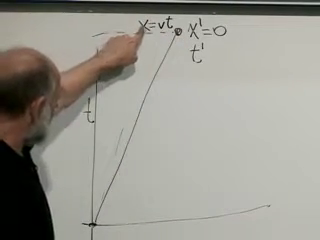
\includegraphics[width=0.72\textwidth]{lecture_04_figure_03.png}
\caption{Gốc chuyển động: $x=vt$, $x'=0$ và trục $t'$ là ba mô tả của cùng một đường thế giới.}
\lectureframe{00:48:18}
\end{figure}

Áp dụng khoảng bất biến giữa gốc chung và một điểm muộn hơn trên đường thế giới đó:
\begin{align}
t'^2-x'^2&=t^2-x^2,\\
t'^2&=t^2-v^2t^2,\\
t'&=t\sqrt{1-v^2}.
\label{eq:l4-time-dilation-natural}
\end{align}
Khi khôi phục $c$,
\begin{equation}
\Delta\tau=\Delta t\sqrt{1-\frac{v^2}{c^2}}
=\frac{\Delta t}{\gamma},
\qquad
\gamma=\frac{1}{\sqrt{1-v^2/c^2}}.
\label{eq:l4-time-dilation}
\end{equation}

\begin{figure}[H]
\centering
\includegraphics[width=0.73\textwidth]{lecture_04_figure_09.png}
\caption{Kết quả giãn thời gian trên bảng: đồng hồ chuyển động tích lũy $t'=t\sqrt{1-v^2}$ trong đơn vị với $c=1$.}
\lectureframe{00:50:45}
\end{figure}

Quan sát viên đứng yên nói rằng đồng hồ chuyển động chạy chậm. Tính tương hỗ đòi hỏi quan sát viên chuyển động cũng nói điều như vậy về các đồng hồ đứng yên. Không có mâu thuẫn nào, vì hai mô tả đang so sánh những cặp sự kiện ở xa khác nhau.

Thật vậy, một giá trị không đổi của $t'$ trong phương trình~\eqref{eq:l4-lorentz-natural} thỏa
\begin{equation}
t-vx=\text{constant}.
\label{eq:l4-simultaneity}
\end{equation}
Các đường đồng thời của quan sát viên chuyển động bị nghiêng so với các đường ngang $t=\text{constant}$. Mỗi quan sát viên gọi một tập hợp khác của các số chỉ đồng hồ ở xa là đồng thời. Một khi giữ rõ sự khác biệt đó, sự chạy chậm tương hỗ của các đồng hồ là nhất quán.

\begin{figure}[H]
\centering
\begin{tikzpicture}[x=1cm,y=1cm]
\draw[->] (0,0) -- (0,4.2) node[above] {$t$};
\draw[->] (0,0) -- (5.2,0) node[right] {$x$};
\draw[thick,->] (0,0) -- (2.4,3.8) node[above] {$x'=0$};
\draw[dashed] (0,2.8) -- (4.8,2.8)
  node[right] {$t=\mathrm{const}$};
\draw[thick] (0.15,1.05) -- (4.7,2.35)
  node[right] {$t'=\mathrm{const}$};
\draw[thick] (3.4,0) -- (3.4,3.8);
\fill (3.4,2.8) circle (0.045);
\fill (3.4,1.98) circle (0.045);
\end{tikzpicture}
\caption{Sự giãn thời gian tương hỗ so sánh các số chỉ đồng hồ trên những lát cắt đồng thời khác nhau.}
\end{figure}

\section{Các quỹ đạo của cặp song sinh}

Hai người song sinh bắt đầu tại cùng một sự kiện. Một người ở lại tại $x=0$. Người kia đi ra xa với tốc độ $v$, đảo chiều, rồi trở về với cùng tốc độ ấy. Khi gặp lại nhau, họ so sánh mọi quá trình vật lý có thể đóng vai trò đồng hồ: đồng hồ đeo tay, nhịp tim, trao đổi chất, hay chính sự lão hóa.

Giả sử mỗi nửa chuyến đi kéo dài thời gian tọa độ $T$ trong hệ của người ở nhà. Thời gian riêng của người ở nhà là
\begin{equation}
\tau_{\mathrm{home}}=2T.
\end{equation}
Sự kiện quay đầu có tọa độ $(vT,T)$. Vì vậy chặng đi đầu đóng góp
\begin{align}
\tau_{\mathrm{leg}}
&=\sqrt{T^2-v^2T^2}
=T\sqrt{1-v^2}.
\end{align}
Chặng về đóng góp cùng một lượng, do đó
\begin{equation}
\tau_{\mathrm{travel}}=2T\sqrt{1-v^2}<2T.
\label{eq:l4-twin}
\end{equation}

\begin{figure}[H]
\centering
\includegraphics[width=0.73\textwidth]{lecture_04_figure_10.png}

\vspace{0.8em}

\begin{tikzpicture}[x=1.1cm,y=1cm]
\draw[->] (-0.2,0) -- (3.4,0) node[right] {$x$};
\draw[->] (0,-0.1) -- (0,4.4) node[above] {$t$};
\draw[very thick] (0,0) -- (0,4);
\draw[very thick] (0,0) -- (2.2,2) -- (0,4);
\draw[dashed] (0,2) -- (2.2,2);
\node[left] at (0,2) {$T$};
\node[left] at (0,4) {$2T$};
\node[below right] at (1.1,1.0) {$v$};
\node[above right] at (1.1,3.0) {$-v$};
\end{tikzpicture}
\caption{Đường thế giới của người ở nhà và hai chặng chuyển động. Thời gian riêng của chúng khác nhau vì chúng là những quỹ đạo khác nhau xuyên qua không-thời gian.}
\lectureframe{00:59:35}
\end{figure}

Không có mâu thuẫn nào trong việc tuổi tác không bằng nhau. Quỹ đạo chuyển động có một chỗ rẽ và không liên hệ với quỹ đạo thẳng của người ở nhà bởi một phép đối xứng của một hệ quy chiếu quán tính duy nhất. Trong hình học Euclid thông thường, một đường thẳng và một đường gãy giữa hai điểm cũng có độ dài khác nhau. Hình học Minkowski đảo ngược chuyện đường nào có khoảng lớn hơn, nhưng sự so sánh vẫn là hình học.

\section{Gia tốc và đồng hồ lý tưởng}

\begin{classroomqa}
\audiencequestion{Tại chỗ quay đầu, vật lý là khác đi và người du hành chịu gia tốc. Điều đó có làm mất hiệu lực của phép tính đồng hồ không?
\lecturetimestamp{01:02:19}}
\lecturerresponse{Gia tốc là có thật và giúp nhận diện tính bất đối xứng; không nên tìm cách gạt nó đi. Góc nhọn chỉ là một hình vẽ lý tưởng hóa và có thể được bo tròn thành một chỗ rẽ hữu hạn. Giả thiết vật lý bổ sung là một đồng hồ đủ nhỏ, chế tạo tốt sẽ không nhạy với gia tốc vừa phải và tiếp tục ghi thời gian riêng. Một đồng hồ lớn hoặc mong manh có thể bị biến dạng hay hỏng, nhưng đó là khuyết tật của cơ cấu chứ không phải của khoảng không-thời gian.}
\end{classroomqa}

Giả thiết đồng hồ lý tưởng này không được suy ra chỉ từ riêng phép biến đổi Lorentz. Nó được kiểm nghiệm thông qua ứng xử của các cơ cấu đồng hồ thực tế. Một nguyên tử là một xấp xỉ tốt hơn nhiều so với một chiếc đồng hồ rộng hàng trăm dặm, vì cơ cấu gọn nhỏ khó bị làm méo hơn dưới gia tốc hoặc trọng lực. Chỉ viện dẫn thuyết tương đối rộng bằng tên gọi cũng không loại bỏ được vấn đề vật lý này; người ta vẫn phải biết cơ cấu đã chọn đáp ứng với môi trường của nó như thế nào.

\begin{classroomqa}
\audiencequestion{Có thể chia một quỹ đạo gia tốc thành những khoảng ngắn mà trên đó phân tích quán tính vẫn còn đúng hay không?\lecturetimestamp{01:09:08}}
\lecturerresponse{Có. Hãy chia đường cong thành các đoạn ngắn, gần như thẳng, tính thời gian riêng trên từng đoạn rồi cộng các kết quả lại. Đây là phép tương tự trong không-thời gian của việc tìm độ dài của một đường cong thông thường từ nhiều đoạn thẳng nhỏ. Trong giới hạn liên tục,
\[
\tau=\int \sqrt{1-\frac{v(t)^2}{c^2}}\,dt,
\]
cho chuyển động trong không-thời gian phẳng được mô tả trong một hệ tọa độ quán tính.}
\end{classroomqa}

\section{Cặp song sinh thấy gì}

Có thể xác định bằng thao tác thực nghiệm các số đọc cuối cùng của đồng hồ bằng cách gửi các xung ánh sáng. Đánh dấu các khoảng 1 giây của thời gian riêng trên cả hai đường thế giới và cho mỗi người song sinh phát ra một xung ở mỗi mốc. Trong chặng đi ra xa, các xung nhận từ người kia thưa ra. Trong chặng quay về, chúng đến dồn lại. Đây là hiệu ứng Doppler tương đối tính được biểu diễn trực tiếp trên biểu đồ không-thời gian.

\begin{figure}[H]
\centering
\includegraphics[width=0.73\textwidth]{lecture_04_figure_11.png}
\caption{Các tín hiệu ánh sáng được trao đổi giữa đường thế giới của người ở nhà và của người du hành. Các tín hiệu đến thưa trong chặng đi ra xa và dồn lại trong chặng quay về vẫn tính đủ mọi xung được phát ra.}
\lectureframe{01:12:55}
\end{figure}

Không có hệ quy chiếu nào trong câu chuyện này biến mất. Mỗi người quan sát rốt cuộc đều nhận được tất cả các xung do người kia phát ra, nhưng tốc độ thu nhận của họ phụ thuộc vào chuyển động tương đối. Sự dịch đỏ trên chặng đi và sự dịch xanh trên chặng về không phải là các hiệu ứng kéo dài trong những khoảng thời gian bằng nhau trên hai chặng, nên việc đếm tất cả các xung nhận được phù hợp với phép so sánh thời gian riêng.

\begin{classroomqa}
\audiencequestion{Nếu người du hành quay về nhận ánh sáng bị dịch xanh, liệu người đó có thể thu được nhiều năng lượng hơn nguồn đã phát ra không?\lecturetimestamp{01:13:50}}
\lecturerresponse{Câu hỏi đó đòi hỏi định nghĩa tương đối tính về năng lượng và tính phụ thuộc hệ quy chiếu của nó, những điều chúng ta vẫn chưa trình bày. Đó là một câu hỏi hợp lý, nhưng chỉ riêng tọa độ và số đếm xung là không đủ để quyết định việc hạch toán năng lượng, đặc biệt đối với một người quan sát có gia tốc. Vì vậy nên hoãn câu trả lời lại thay vì đoán mò.}
\end{classroomqa}

\section{Một phương không gian khép kín}

\begin{classroomqa}
\audiencequestion{Giả sử một phương không gian là khép kín. Liệu một người song sinh có thể chuyển động đều theo phương ấy, trở về điểm xuất phát và hoàn toàn tránh được gia tốc không? Khi đó điều gì phân biệt hai người?\lecturetimestamp{01:15:14}}
\lecturerresponse{Không gian nên được hình dung một cách nội tại như một hình trụ, chứ không phải như một tấm bị uốn bên trong một không gian lớn hơn; không nhất thiết phải có gia tốc hướng tâm. Tuy vậy, người quan sát quay về vẫn đối mặt với sự kiện toàn cục rằng cùng một vị trí lặp lại. Điều đó cho thấy có một sự bất đối xứng, nhưng một câu trả lời đầy đủ đòi hỏi phải xử lý cẩn thận thuyết tương đối hẹp với phép đồng nhất hóa không gian này. Ở đây câu hỏi ấy được để ngỏ thay vì được trả lời ngẫu hứng.}
\end{classroomqa}

\begin{figure}[H]
\centering
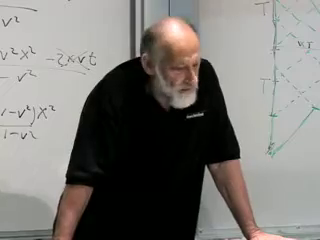
\includegraphics[width=0.72\textwidth]{lecture_04_figure_04.png}

\vspace{0.8em}

\begin{tikzpicture}[x=1cm,y=1cm]
\draw[thick] (0,0) ellipse (1.3 and 0.35);
\draw[thick] (-1.3,0) -- (-1.3,-3.1);
\draw[thick] (1.3,0) -- (1.3,-3.1);
\draw[thick] (0,-3.1) ellipse (1.3 and 0.35);
\draw[->,very thick] (0.0,0.38) arc (90:-210:1.38 and 0.42);
\node[right] at (1.65,-1.5) {compact spatial direction};
\end{tikzpicture}
\caption{Câu hỏi về không gian khép kín như được vẽ trên bảng, với một hình trụ nội tại thuần túy. Đây là một câu hỏi về phép đồng nhất hóa toàn cục, không phải về chuyển động quanh một hình trụ được nhúng trong một chiều hướng kính phụ thêm.}
\lectureframe{01:17:56}
\end{figure}

\section{Độ dài được đo trên một lát cắt đồng thời}

Đối với một bài toán trong thuyết tương đối hẹp, trước hết hãy vẽ bức tranh không-thời gian. Xét một thước mét đứng yên trong hệ không dấu phẩy, với hai đầu tại $x=0$ và $x=1$. Khi thời gian trôi đi, hai đầu ấy vạch nên các đường thế giới thẳng đứng. Cây thước quét ra một dải giữa chúng.

Người quan sát chuyển động phải đo cả hai đầu tại cùng một giá trị của thời gian $t'$ trong hệ chuyển động. Từ phương trình~\eqref{eq:l4-simultaneity}, lát cắt đi qua gốc tọa độ với $t'=0$ thỏa mãn \begin{equation}
t=vx
\end{equation} khi dùng đơn vị $c=1$. Nó cắt đầu bên phải $x=1$ tại $t=v$.

\begin{figure}[H]
\centering
\includegraphics[width=0.73\textwidth]{lecture_04_figure_12.png}

\vspace{0.8em}

\begin{tikzpicture}[x=1.55cm,y=1.15cm]
\draw[->] (-0.5,0) -- (3.1,0) node[right] {$x$};
\draw[->] (0,0) -- (0,3.8) node[above] {$t$};
\draw[very thick,red] (0,0) -- (0,3.3);
\draw[very thick,red] (2.15,0) -- (2.15,3.3);
\fill[red!12] (0,0) rectangle (2.15,3.3);
\draw[very thick,green!50!black] (0,0) -- (1.2,3.1)
  node[above] {$x=vt$};
\draw[very thick,blue] (0,0) -- (2.15,1.15)
  node[right] {$t'=0$};
\fill (2.15,1.15) circle (0.045);
\node[right] at (2.22,1.35) {$(x,t)=(1,v)$};
\node[below] at (2.15,0) {$1$};
\end{tikzpicture}
\caption{Một thanh đứng yên quét ra một dải không-thời gian. Độ dài mà người quan sát chuyển động đo được là khoảng cách giữa hai đầu của nó trên một lát cắt $t'=\mathrm{const}$.}
\lectureframe{01:24:20}
\end{figure}

Độ tách giữa hai đầu được chọn là kiểu không gian, nên dùng dạng không gian mang dấu dương của bất biến:
\begin{equation}
x'^2-t'^2=x^2-t^2.
\end{equation}
Tại đầu mút được chọn, $t'=0$, $x=1$ và $t=v$. Do đó
\begin{align}
x'^2&=1-v^2,\\
x'&=\sqrt{1-v^2}.
\end{align}
Vì vậy, một độ dài riêng $L$ được đo trong hệ chuyển động là
\begin{equation}
L'=L\sqrt{1-v^2/c^2}=\frac{L}{\gamma}.
\label{eq:l4-length-contraction}
\end{equation}

\begin{figure}[H]
\centering
\includegraphics[width=0.76\textwidth]{lecture_04_figure_13.png}
\caption{Phép dựng hoàn chỉnh cho co độ dài và kết quả trên bảng $x'=\sqrt{1-v^2}$ đối với một độ dài riêng đơn vị.}
\lectureframe{01:28:10}
\end{figure}

Mệnh đề đối ứng cũng đúng: người quan sát trên sân ga gán một độ dài ngắn hơn cho thước mét theo phương dọc của đoàn tàu. Một lần nữa, hai người quan sát chọn những sự kiện đầu mút đồng thời khác nhau, nên tính đối ứng này không mâu thuẫn.

\section{Các câu hỏi ở phần cuối}

\begin{classroomqa}
\audiencequestion{Ngoài ánh sáng ra, có gì lan truyền với tốc độ ánh sáng không? Cụ thể, còn hấp dẫn thì sao?\lecturetimestamp{01:29:29}}
\lecturerresponse{Thuyết tương đối rộng dự đoán các sóng hấp dẫn lan truyền với $c$. Vào thời điểm của bài giảng này, bằng chứng chỉ đến gián tiếp từ các hệ như pulsar đôi; khi ấy sóng hấp dẫn vẫn chưa được phát hiện trực tiếp.\editorialnote{Tình hình thực nghiệm đã thay đổi sau bài giảng 2006 này. LIGO đã trực tiếp phát hiện GW150914 vào 2015, và việc quan sát đồng thời GW170817 cùng đối ứng điện từ của nó vào 2017 cho thấy tốc độ lan truyền của hấp dẫn và ánh sáng khớp nhau tới mức sai khác chỉ vài phần trên $10^{15}$. Xem \url{https://ligo.org/detections/gw150914/} và \url{https://doi.org/10.1103/PhysRevLett.119.251302}.}}
\end{classroomqa}

\begin{classroomqa}
\audiencequestion{Một phi hành gia có thể vượt qua một quãng đường dài nhiều năm ánh sáng trong một thời gian riêng nhỏ hơn giá trị của quãng đường đó khi biểu diễn bằng năm ánh sáng không? Điều đó có đồng nghĩa với chuyển động nhanh hơn ánh sáng không?\lecturetimestamp{01:30:38}}
\lecturerresponse{Thời gian riêng của phi hành gia là $\sqrt{\Delta t^2-\Delta x^2}$, nhỏ hơn thời gian tọa độ $\Delta t$. Trong hệ quán tính của phi hành gia, khoảng cách giữa các ngôi sao bị co Lorentz. Các ngôi sao chuyển động với vận tốc $-v$, chứ không nhanh hơn ánh sáng; đơn giản chỉ là khoảng cách đã co cần vượt qua nhỏ hơn.}
\end{classroomqa}

Nếu phi hành gia bắt đầu từ trạng thái đứng yên rồi gia tốc, mô tả sẽ thay đổi qua một chuỗi các hệ quán tính tức thời. Khoảng cách gán cho các ngôi sao có thể thay đổi trong quá trình chuyển tiếp đó. Không thể áp dụng một phép biến đổi Lorentz cố định cho toàn bộ lịch sử có gia tốc, nhưng tổng thời gian riêng vẫn được xác định bằng cách cộng các đóng góp dọc theo đường thế giới. Điều tương tự cũng áp dụng cho người song sinh trong tình huống thực tế, người phóng đi, quay đầu và giảm tốc, chứ không phải sinh ra đã ở tốc độ hành trình.

\begin{classroomqa}
\audiencequestion{Những điều khó hiểu này có phải do việc coi thời gian là đặc biệt không? Có nhất thiết phải gọi nó là chiều thứ tư không?\lecturetimestamp{01:36:43}}
\lecturerresponse{Không nhất thiết phải bắt đầu bằng khẩu hiệu rằng thời gian là chiều thứ tư. Chính phép biến đổi Lorentz buộc không gian và thời gian trộn lẫn, còn khoảng $t^2-x^2-y^2-z^2$ xem chúng như những phần của một hình học thống nhất với dấu khác nhau cho thời gian và không gian. Ở vận tốc thấp, sự trộn lẫn ấy trở nên không đáng kể và trực giác Newton quen thuộc quay trở lại. Tuy nhiên, ở vận tốc tương đối tính, không gian và thời gian không thể được xem là tách rời nhau một cách cơ bản.}
\end{classroomqa}

Vì vậy, sự giãn thời gian, co độ dài, việc so sánh hai người song sinh và thời gian hành trình rút ngắn không phải là những mẹo tách biệt. Tất cả đều theo từ ba thói quen: xác định các sự kiện đang được so sánh, vẽ hình học không-thời gian của chúng và dùng khoảng bất biến.
\chapter{Quả cầu lửa, hệ quy chiếu và bốn-vectơ}

Chúng ta bắt đầu với một câu hỏi còn lại từ cuộc thảo luận về các va chạm năng lượng cao. Một va chạm của hai hạt nhân nặng tạo ra một đối tượng biến đổi dữ dội, chứ không phải một lỗ đen thiên văn yên ắng. Vậy thì mô tả va chạm đó bằng một chân trời có thể có nghĩa là gì? Câu trả lời dẫn qua một bức tranh năm chiều về vật chất ở chế độ ghép mạnh, một loạt câu hỏi thực tiễn về máy gia tốc, và cuối cùng quay trở lại hình học của thuyết tương đối hẹp. Đến cuối cùng, vận tốc và động lượng đã trở thành các bốn-vectơ, còn năng lượng đã đứng bên cạnh ba thành phần của động lượng.

\section{Một quả cầu lửa trong chiều không gian thứ năm}

\begin{classroomqa}
\audiencequestion{Đối tượng được tạo ra trong va chạm là không ổn định và thay đổi hình dạng. Làm sao một vật thể phức tạp như vậy lại có thể được gọi là lỗ đen?}
\lecturerresponse{Hãy hình dung một phương không gian thứ năm chạy giữa một cái sàn và một cái trần. Trọng lực theo phương đó kéo các kích thích về phía sàn. Va chạm đặt xuống đó một khối năng lượng nóng; khối ấy lan ra và đổi dạng, nhưng vẫn có thể có chân trời, nhiệt độ và entropy.}
\end{classroomqa}

Hãy tưởng tượng các hạt, hay hình tượng hơn là những sợi dây nhỏ, chuyển động trong thế giới năm chiều này. Những kích thích rơi xuống sàn xuất hiện trong bốn chiều dưới dạng các hadron: proton, neutron, meson và các đối tượng hợp thành mở rộng khác. Những kích thích gắn gần trần thì có vẻ cơ bản hơn. Vì thế, vị trí theo phương thẳng đứng là một cách hình học để mã hóa thang đo: sàn biểu diễn chế độ hadron ở khoảng cách lớn, còn trần biểu diễn các bậc tự do ở khoảng cách ngắn.

Khi hai hadron va chạm, hai đối tượng ở gần sàn đập vào nhau và làm bắn tóe ra một lượng năng lượng lớn. Kết quả không phải là một vật rắn. Nó là một khối nóng mang chân trời, một kiểu vũng năng lượng trong trường hấp dẫn năm chiều. Nó không phải là một lỗ đen thiên văn trong không gian bốn chiều thông thường, cũng không phải là một lỗ đen ở thang Planck gắn với trần. Nó là mô tả hấp dẫn của quả cầu lửa tương tác mạnh gần sàn.

Ở năng lượng cao, các hạt nhân tới bị co Lorentz thành những chiếc bánh dẹt mỏng. Chúng va chạm, gửi năng lượng của mình vào một vùng nhỏ và tạo ra một chất lưu lan ra và tiến tới cân bằng. Độ nhớt nhỏ của nó là một trong những đặc điểm gây ngạc nhiên của plasma quark--gluon. Trong mô tả năm chiều, cùng một sự tiến triển đó là sự thư giãn của một chân trời bị méo dạng.

\begin{figure}[H]
\centering
\includegraphics[width=0.82\textwidth]{lecture_05_figure_01.png}
\caption{Bức tranh sàn-và-trần của chiều thứ năm. Khối trung tâm mang chân trời lan dọc theo sàn sau va chạm.}
\lectureframe{00:04:22}
\end{figure}

Một chân trời không tồn tại mãi mãi. Bức xạ Hawking mang năng lượng đi, và trong mô tả bốn chiều, bức xạ ấy chính là cơn mưa các hadron thông thường xuất hiện từ va chạm. Hàng nghìn vệt ghi trong một sự kiện của đầu dò, theo ngôn ngữ này, là các hạt bị sôi tách ra khỏi lỗ đen đối ngẫu.

\subsection{Chiều phụ có thực không?}

\begin{classroomqa}
\audiencequestion{Chiều thứ năm có phải là một chiều không gian không, và đường được vẽ giữa sàn và trần có thực sự kéo dài theo phương đó không?}
\lecturerresponse{Có. Nó có tính không gian, và bề mặt được vẽ trong hình học năm chiều ấy là một chân trời. Việc ta gọi phương phụ đó là ``thực'' hay xem nó như một mô tả toán học tương đương là một câu hỏi sâu hơn.}
\end{classroomqa}

Điều hữu ích không phải là nói rằng hấp dẫn thay thế sắc động lực học lượng tử. Đúng hơn, hai ngôn ngữ có thể mô tả cùng một vật lý. Trong ngôn ngữ bốn chiều có một quả cầu lửa nóng gồm quark và gluon, không có trường hấp dẫn thông thường nào. Trong ngôn ngữ năm chiều có hấp dẫn và một chân trời. Nếu sự tương ứng là đúng, thì một phép tính QCD đúng nghĩa và phép tính hấp dẫn đối ngẫu phải cho cùng kết quả ở mọi nơi mà cả hai đều có thể thực hiện được.

\begin{classroomqa}
\audiencequestion{QCD không có hấp dẫn cũng không có chân trời. Bức tranh lỗ đen có đang thêm vào vật lý mới không, hay nó chỉ mô tả lại quả cầu lửa?}
\lecturerresponse{Trong bốn chiều, đó là một plasma quark và gluon; trong hiện thân năm chiều, nó có một mô tả hấp dẫn với một chân trời. Lợi thế nằm ở tính toán. QCD ở chế độ ghép mạnh cực kỳ khó, trong khi một số tính chất của chân trời---đặc biệt là độ nhớt---lại tương đối dễ tính.}
\end{classroomqa}

Sự phân biệt giữa ``chiều thực'' và ``phép tương tự toán học'' không nhất thiết phải được giải quyết trước khi mô tả ấy trở nên hữu ích. Một cấu trúc có được một cách hiểu vật lý khi nó kết hợp với các biến khác thành một hệ quy luật đơn giản hơn, mạch lạc hơn. Tuy vậy, không nên nói quá: các ứng dụng của đối ngẫu chuẩn/hấp dẫn đối với plasma quark--gluon được quan sát chỉ là những mô hình của động lực học ghép mạnh, chứ không phải là bằng chứng rằng QCD trong thế giới thực có một đối ngẫu hấp dẫn chính xác đã biết.\editorialnote{Sự bảo lưu này làm rõ vị thế hiện nay của ứng dụng QCD; nó không làm thay đổi cơ chế năm chiều được phát triển ở đây.}

\section{Vì sao máy va chạm cho hai chùm hạt va nhau}

Những câu hỏi bây giờ trở nên thực tiễn. Vì sao dùng hai chùm đang chuyển động thay vì một chùm đơn và một bia đứng yên? Vì sao máy gia tốc tròn lại lớn đến vậy? Vì sao electron và proton được xử lý khác nhau? Tất cả những câu hỏi ấy đều là những câu hỏi về năng lượng tương đối tính.

\begin{classroomqa}
\audiencequestion{Vì sao cho hai chùm va chạm nhau thay vì bắn một chùm năng lượng cao vào một bia đứng yên?}
\lecturerresponse{Điều tạo ra hạt mới là năng lượng sẵn có trong hệ quy chiếu khối tâm. Hai chùm tương đối tính bằng nhau và ngược chiều có tổng động lượng bằng không, nên về cơ bản hầu như toàn bộ năng lượng của chúng đều sẵn cho va chạm. Một bia cố định buộc phần lớn năng lượng của chùm tới phải còn lại dưới dạng chuyển động của khối tâm.}
\end{classroomqa}

Đối với hai hạt siêu tương đối tính có động lượng ngược chiều với độ lớn \(p\), ước lượng ở mức bài giảng trong các đơn vị \(c=1\) là
\begin{equation}
E_{\mathrm{cm}}^{\mathrm{collider}}\simeq 2p.
\end{equation}
Ước lượng tương ứng cho trường hợp bia cố định chỉ tăng theo căn bậc hai của động lượng chùm,
\begin{equation}
E_{\mathrm{cm}}^{\mathrm{fixed}}\sim \sqrt{mp}.
\end{equation}
Điều cốt yếu là quy luật tỉ lệ, chứ không phải hệ số số học đã được lược bỏ: gấp đôi năng lượng chùm thì gấp đôi năng lượng va chạm của collider, nhưng năng lượng khối tâm của cấu hình bia cố định chỉ tăng theo căn bậc hai.

Phép tính bất biến làm cho phép so sánh trở nên chính xác. Nếu \(P_1\) và \(P_2\) là các bốn-động lượng tới, thì
\begin{equation}
s=(P_1+P_2)^2,
\qquad E_{\mathrm{cm}}=\sqrt{s}.
\end{equation}
Đối với hai chùm ngược chiều có cùng năng lượng \(E\), các động lượng không gian triệt tiêu nhau và \(\sqrt{s}=2E\). Đối với một hạt bắn tới có năng lượng \(E\gg m\) đập vào một bia cùng khối lượng đang đứng yên,
\begin{equation}
s=2m^2+2mE,
\qquad
\sqrt{s}\simeq \sqrt{2mE}
\qquad (c=1).
\end{equation}
Suy dẫn ngắn gọn bằng bất biến này cung cấp hệ số đã bị lược bỏ trong ước lượng bằng lời.\editorialnote{Phần suy dẫn được đưa vào để lập luận về quy luật tỉ lệ trong bài giảng có thể được tái lập.}

\begin{classroomqa}
\audiencequestion{Có lý do cơ bản nào khiến một máy gia tốc tròn phải lớn đến vậy không? Có thể chỉ cho cùng một chùm đó lưu thông qua một máy nhỏ hơn nhiều vòng hơn không?}
\lecturerresponse{Trường và vật liệu đặt ra các giới hạn. Một hạt chỉ nhận được một độ tăng năng lượng hữu hạn trên mỗi mét, nên một máy năng lượng cao hơn cần một chiều dài gia tốc hiệu dụng lớn hơn. Một vòng tròn chật hơn cũng đòi hỏi gia tốc ngang lớn hơn, và một điện tích bị gia tốc thì bức xạ. Nếu vòng quá nhỏ, chùm sẽ bức xạ năng lượng nhanh ngang với tốc độ máy cung cấp nó.}
\end{classroomqa}

Quan hệ bẻ cong xấp xỉ là
\begin{equation}
p=qBR,
\end{equation}
nên với từ trường \(B\) cố định, động lượng \(p\) lớn hơn đòi hỏi bán kính \(R\) lớn hơn. Các hốc cộng hưởng tần số vô tuyến thực hiện công làm tăng năng lượng chùm; còn nam châm bẻ cong và hội tụ chùm. Bài học tổng quát vẫn là điều đã nói trên bảng: cường độ trường và tổn hao bức xạ ngăn chúng ta nén một máy gia tốc có năng lượng tùy ý lớn vào một vòng nhỏ.

Chuyển động tròn có gia tốc ngay cả khi tốc độ không đổi vì vận tốc đổi hướng. Một điện tích bị gia tốc phát ra bức xạ synchrotron. Máy gia tốc thẳng tránh được tổn hao do bẻ cong liên tục, mặc dù bản thân các cú đẩy gia tốc ngắn ấy theo nghĩa đen không phải là hoàn toàn không bức xạ. Máy tròn chấp nhận cái giá của sự bẻ cong để đổi lấy việc tái sử dụng cùng một thiết bị trên mỗi vòng quỹ đạo.

\begin{classroomqa}
\audiencequestion{Vì sao electron gắn với máy gia tốc thẳng ở SLAC, trong khi các máy va chạm tròn năng lượng cao lại dùng proton hoặc các hadron khác?}
\lecturerresponse{Electron nhẹ hơn rất nhiều. Ở cùng một năng lượng cao, hệ số Lorentz của chúng lớn hơn nhiều, và gia tốc tròn khiến chúng bức xạ mạnh hơn hẳn. Các proton nặng hơn có thể quay vòng lặp đi lặp lại, nhận thêm năng lượng ở mỗi lần đi qua, trước khi tổn hao synchrotron trở nên không thể chấp nhận được.}
\end{classroomqa}

Với năng lượng và bán kính vòng cố định, công suất bức xạ phụ thuộc rất dốc vào khối lượng hạt,
\begin{equation}
P_{\mathrm{sync}}\propto \frac{E^4}{m^4R^2}.
\end{equation}
Đó là vì sao sự khác biệt electron--proton sắc nét hơn nhiều so với điều mà cụm từ ``hạt nhẹ hơn chuyển động nhanh hơn'' có thể gợi ra: cả hai chùm đều có thể đã cực kỳ gần \(c\), nhưng hệ số Lorentz và tổn hao bức xạ của chúng rất khác nhau.\editorialnote{Quan hệ bẻ cong và quy luật tỉ lệ synchrotron làm cho lập luận định tính về máy gia tốc trong bài giảng trở nên chính xác; chúng đã không được triển khai trên bảng.}

\begin{classroomqa}
\audiencequestion{Vì sao không gia tốc hadron trên một đường thẳng luôn?}
\lecturerresponse{Có thể. Khó khăn nằm ở chiều dài. Trong một vòng, cùng một hạt đi qua các cấu trúc gia tốc nhiều lần; một máy hadron thẳng tương đương sẽ phải dài khổng lồ. Giải pháp thỏa hiệp hữu ích là một vòng lớn, đủ lớn để bức xạ proton vẫn còn chấp nhận được.}
\end{classroomqa}

Những câu hỏi về máy gia tốc này cho thấy chính xác vì sao các quy tắc Newton là không đủ. Bây giờ ta quay lại thuyết tương đối hẹp và xây dựng ngôn ngữ khiến những so sánh như vậy trở nên có hệ thống.

\section{Ga-ra và chiếc limousine}

Hãy xét một ga-ra dài khoảng 12 foot và một chiếc limousine kéo dài khoảng 20 foot. Người lái tăng tốc cho đến khi chiếc limousine bị co Lorentz, hy vọng nó sẽ lọt vào. Trong hệ quy chiếu của ga-ra, chiếc limousine đang chuyển động ngắn hơn, nên điều đó có vẻ khả thi. Tuy nhiên, trong hệ quy chiếu của limousine, ga-ra đang chuyển động ngắn hơn, nên điều đó có vẻ bất khả thi. Toàn bộ chiếc limousine có thể nằm trong ga-ra hay không?

Mở cả hai cửa để việc va vào tường không làm ta phân tâm. Nói rằng chiếc limousine ở trong có nghĩa là đầu trước và đầu sau của nó đều ở trong \emph{đồng thời}. Từ cuối cùng đó chứa trọn toàn bộ câu đố.

Hãy vẽ một giản đồ không-thời gian với \(t\) thẳng đứng và \(x\) nằm ngang. Các tia sáng tạo thành nón ánh sáng \(45^\circ\) trong đơn vị \(c=1\). Ga-ra đứng yên, nên các đường thế giới của hai cánh cửa là thẳng đứng. Đầu trước và đầu sau của chiếc limousine vạch ra hai đường thế giới nghiêng song song. Trục \(t'\) của hệ chuyển động nghiêng về phía nón ánh sáng, và các đường đồng thời của nó song song với trục \(x'\) đã nghiêng.

\begin{figure}[H]
\centering
\includegraphics[width=0.82\textwidth]{lecture_05_figure_02.png}
\caption{Giản đồ không-thời gian ga-ra--limousine hoàn chỉnh. Các đường thẳng đứng giới hạn ga-ra; các đường nghiêng vạch ra hai đầu của chiếc limousine. Các lát cắt ngang và nghiêng biểu diễn các lát đồng thời khác nhau của hai hệ quy chiếu.}
\lectureframe{00:31:05}
\end{figure}

Trong hệ quy chiếu của ga-ra, một đường ngang có thể cắt cả hai đường thế giới của limousine ở giữa hai đường thế giới của ga-ra. Ở thời điểm đó theo ga-ra, phần sau đã vào và phần trước vẫn chưa ra. Chiếc limousine đã co nằm hoàn toàn bên trong.

Trong hệ quy chiếu của limousine, các sự kiện đồng thời liên quan nằm trên một đường nghiêng. Hãy vẽ một đường như vậy đi qua sự kiện tại đó phần sau đi vào. Nó cắt đường thế giới của phần trước sau khi đầu trước đã đi qua cửa xa rồi. Theo tính đồng thời riêng của nó, chiếc limousine không bao giờ nằm hoàn toàn bên trong. Cả hai phát biểu đều đúng vì chúng so sánh những cặp sự kiện khác nhau.

\begin{classroomqa}
\audiencequestion{Hai đường thế giới màu xanh lá và đoạn nằm ngang giữa chúng có tạo thành một hình bình hành không? Đoạn màu đen đó có phải là chiều dài của chiếc xe không?}
\lecturerresponse{Đoạn nằm ngang là chiều dài bị co Lorentz, vì hai đầu mút của nó là đồng thời trong hệ quy chiếu của ga-ra. Độ dài riêng được lấy từ các đầu mút đồng thời trong hệ quy chiếu của xe limousine, trên một đường thẳng song song với \(x'\). Hai phép đo dùng những lát cắt khác nhau qua cùng một cặp đường thế giới.}
\end{classroomqa}

Nếu \(L_0\) là độ dài riêng, thì lát cắt nằm ngang trong hệ quy chiếu ga-ra có độ dài
\begin{equation}
L=\frac{L_0}{\gamma},
\qquad
\gamma=\frac{1}{\sqrt{1-v^2/c^2}}.
\end{equation}
Chỉ riêng công thức thì không giải quyết được nghịch lý. Hình vẽ làm được điều đó, vì nó cho thấy những sự kiện nào đã được đem so sánh. Bất cứ khi nào một bài toán đố về thuyết tương đối dường như cho ra hai đáp án không tương thích, hãy tìm xem từ ``đồng thời'' có đang được dùng ngầm hay không.

\section{Bốn tọa độ và hai vị trí của chỉ số}

Để chuyển từ các nghịch lý sang các định luật chuyển động, ta cần một ký hiệu ghi nhớ hình học. Gom các tọa độ lại thành
\begin{equation}
(X^1,X^2,X^3,X^0)=(x,y,z,t),
\qquad X^\mu=(x,y,z,t),
\end{equation}
trong đó \(\mu\) chạy qua \(1,2,3,0\). Thứ tự này đặt thời gian ở cuối trên trang giấy dù chỉ số của nó là \(0\), phù hợp với quy ước được dùng trên bảng.

\begin{classroomqa}
\audiencequestion{Chúng ta có đang đặt \(c=1\) không? Nếu khôi phục các đơn vị thông thường, thì tọa độ thời gian có phải là \(ct\) không?}
\lecturerresponse{Có. Ta đặt \(c=1\) khi triển khai phần hình học và đưa các thừa số \(c\) trở lại khi cần xét thứ nguyên hoặc giới hạn phi tương đối tính. Với đơn vị chiều dài thông thường, tọa độ thời gian là \(ct\).}
\end{classroomqa}

Cùng một vectơ có thể được viết với chỉ số dưới. Với quy ước dấu dùng ở đây,
\begin{equation}
X_\mu=(-x,-y,-z,t).
\end{equation}
Vì vậy, hạ một chỉ số sẽ đảo dấu ba thành phần không gian và giữ nguyên thành phần thời gian. Ví dụ,
\begin{equation}
X^\mu=(3,2,4,10)
\quad\Longrightarrow\quad
X_\mu=(-3,-2,-4,10).
\end{equation}
Đây không phải là hai điểm không-thời gian; chúng là hai dạng thành phần của cùng một đối tượng hình học.

\begin{classroomqa}
\audiencequestion{Những thành phần nào là hiệp biến và phản biến, và các nhãn ấy là chỉ số trên hay chỉ số dưới?}
\lecturerresponse{Các thành phần mang chỉ số trên là phản biến; các thành phần mang chỉ số dưới là hiệp biến. Một mẹo ghi nhớ hữu ích ngay trong lớp là ``co thì thấp, contra thì cao.'' Các nhà vật lý thường đơn giản gọi chúng là chỉ số trên và chỉ số dưới.}
\end{classroomqa}

Ký hiệu này phát huy tác dụng trong phép co bất biến
\begin{equation}
X_\mu X^\mu=t^2-x^2-y^2-z^2.
\label{eq:l5-interval}
\end{equation}
Dưới dạng vi phân, ta có
\begin{equation}
d\tau^2=dt^2-dx^2-dy^2-dz^2
\qquad (c=1).
\label{eq:l5-proper-time}
\end{equation}
Đối với chuyển động kiểu thời gian, \(d\tau\) là thời gian mà một đồng hồ chuyển động dọc theo đường thế giới ghi lại.

Mỗi khi cùng một chỉ số xuất hiện một lần ở trên và một lần ở dưới, ta ngầm hiểu là phải lấy tổng. Quy ước Einstein biến
\begin{equation}
\sum_{\mu}X_\mu X^\mu
\end{equation}
thành biểu thức ngắn hơn trong phương trình~\eqref{eq:l5-interval}. Đây không chỉ đơn thuần là tiết kiệm ký hiệu. Nó ngăn không cho các dấu xen kẽ của hình học Minkowski phải được viết lại bằng tay trong mọi phương trình.

\begin{classroomqa}
\audiencequestion{Có phải \(\tau\) là ký hiệu chuẩn cho thời gian riêng không?}
\lecturerresponse{Có. Ký hiệu \(s\) đôi khi cũng được dùng, nhưng \(\tau\) là một lựa chọn chuẩn cho thời gian riêng.}
\end{classroomqa}

\section{Phép quay như một đối xứng dễ xử lý}

Một phép boost Lorentz trộn lẫn không gian và thời gian. Trước khi khảo sát ma trận đó, hãy xét phép toán quen thuộc hơn là quay các trục không gian. Nếu chuyển động tương đối hướng theo một phương bất kỳ, ta có thể quay các trục cho đến khi phương đó trở thành trục \(x\) mới rồi áp dụng phép boost đã biết. Vì vậy, các phép quay là một phần của cách xây dựng, chứ không phải một đường vòng mang tính trang trí.

Đối với phép quay một góc \(\theta\) quanh trục \(z\),
\begin{align}
x'&=x\cos\theta+y\sin\theta,\nonumber\\
y'&=-x\sin\theta+y\cos\theta,\label{eq:l5-rotation}\\
z'&=z.\nonumber
\end{align}
Khi \(\theta=0\), các phương trình này cho lại \(x'=x\) và \(y'=y\); khi \(\theta=\pi/2\), chúng hoán đổi hai trục với các dấu như dự kiến.

Phép biến đổi này bảo toàn khoảng cách Euclid. Viết
\(c_\theta=\cos\theta\) và \(s_\theta=\sin\theta\),
\begin{align}
x'^2+y'^2
&=(xc_\theta+ys_\theta)^2+(-xs_\theta+yc_\theta)^2\nonumber\\
&=x^2(c_\theta^2+s_\theta^2)
  +y^2(s_\theta^2+c_\theta^2)\nonumber\\
&\quad+2xyc_\theta s_\theta-2xyc_\theta s_\theta\nonumber\\
&=x^2+y^2.
\end{align}
Các hạng chéo triệt tiêu nhau và \(c_\theta^2+s_\theta^2=1\). Vì \(z'=z\),
độ dài đầy đủ \(x^2+y^2+z^2\) là bất biến.

Cũng các phương trình ấy có thể gộp thành một phương trình ma trận:
\begin{equation}
\begin{pmatrix}x'\\y'\\z'\end{pmatrix}
=
\underbrace{\begin{pmatrix}
\cos\theta&\sin\theta&0\\
-\sin\theta&\cos\theta&0\\
0&0&1
\end{pmatrix}}_{M}
\begin{pmatrix}x\\y\\z\end{pmatrix}.
\label{eq:l5-rotation-matrix}
\end{equation}
Theo ký hiệu chỉ số,
\begin{equation}
x'^i=M^i{}_{j}x^j,
\qquad i,j=1,2,3.
\end{equation}

\begin{figure}[H]
\centering
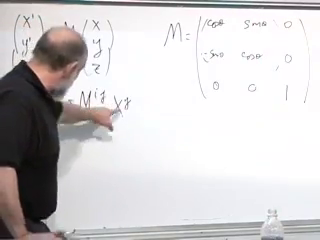
\includegraphics[width=0.82\textwidth]{lecture_05_figure_03.png}
\caption{Phép quay không gian được viết cả dưới dạng phương trình ma trận lẫn dưới ký hiệu chỉ số.}
\lectureframe{01:00:40}
\end{figure}

\section{Ma trận Lorentz và vận tốc hợp thành}

Đối với chuyển động dọc theo \(x\), phép biến đổi Lorentz trong đơn vị \(c=1\) là
\begin{align}
x'&=\gamma_v(x-vt), & y'&=y,\nonumber\\
z'&=z, & t'&=\gamma_v(t-vx),
\end{align}
trong đó
\begin{equation}
\gamma_v=\frac{1}{\sqrt{1-v^2}}.
\end{equation}
Với thứ tự thành phần \((x,y,z,t)\), điều này trở thành
\begin{equation}
\begin{pmatrix}x'\\y'\\z'\\t'\end{pmatrix}
=
\begin{pmatrix}
\gamma_v&0&0&-\gamma_vv\\
0&1&0&0\\
0&0&1&0\\
-\gamma_vv&0&0&\gamma_v
\end{pmatrix}
\begin{pmatrix}x\\y\\z\\t\end{pmatrix}.
\label{eq:l5-lorentz-matrix}
\end{equation}

\begin{figure}[H]
\centering
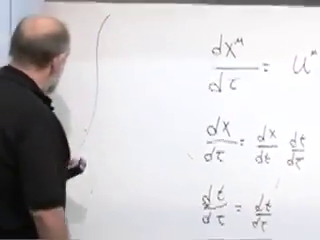
\includegraphics[width=0.82\textwidth]{lecture_05_figure_04.png}
\caption{Ma trận Lorentz \(4\times4\). Chỉ có các thành phần \(x\) và \(t\) trộn lẫn với nhau; \(y\) và \(z\) giữ nguyên.}
\lectureframe{01:04:40}
\end{figure}

Phép nhân ma trận giờ đây trả lời một câu hỏi vật lý. Giả sử một quan sát viên chuyển động với vận tốc \(v\) so với chúng ta và một người thứ ba chuyển động với vận tốc \(u\) so với quan sát viên đó, tất cả đều dọc theo cùng một trục. Động học Newton sẽ cho \(w=u+v\), điều này sẽ cho phép hai vận tốc \(3c/4\) hợp lại thành \(3c/2\). Thuyết tương đối phải cho một quy tắc khác.

Phần tác dụng của phép boost là ma trận \(2\times2\)
\begin{equation}
B(v)=\gamma_v
\begin{pmatrix}1&-v\\-v&1\end{pmatrix}.
\end{equation}
Ghép hai phép boost lại cho
\begin{align}
B(u)B(v)
&=\gamma_u\gamma_v
\begin{pmatrix}1&-u\\-u&1\end{pmatrix}
\begin{pmatrix}1&-v\\-v&1\end{pmatrix}\nonumber\\
&=\gamma_u\gamma_v
\begin{pmatrix}
1+uv&-(u+v)\\
-(u+v)&1+uv
\end{pmatrix}.
\label{eq:l5-composed-boost}
\end{align}
Tỷ số giữa một phần tử ngoài đường chéo và một phần tử trên đường chéo xác định vận tốc của phép boost kết quả:
\begin{equation}
w=\frac{u+v}{1+uv}
\qquad(c=1).
\end{equation}
Khôi phục thứ nguyên,
\begin{equation}
w=\frac{u+v}{1+uv/c^2}.
\label{eq:l5-velocity-addition}
\end{equation}

\begin{figure}[H]
\centering
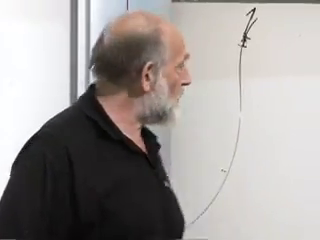
\includegraphics[width=0.82\textwidth]{lecture_05_figure_05.png}
\caption{Ma trận của phép boost hợp thành và vận tốc
\(w=(u+v)/(1+uv)\) trong đơn vị tự nhiên.}
\lectureframe{01:15:35}
\end{figure}

Nếu \(u\) và \(v\) đều gần \(c\), thì tử số tiến tới \(2c\) còn mẫu số tiến tới \(2\), nên \(w\) tiến tới \(c\), chứ không phải \(2c\). Nói tổng quát hơn, phương trình~\eqref{eq:l5-velocity-addition} ánh xạ các đầu vào dưới tốc độ ánh sáng thành một kết quả cũng dưới tốc độ ánh sáng. Phép nhân ma trận đã tự động mã hóa giới hạn tốc độ.

\section{Bốn-vectơ và sự thất bại của vận tốc thông thường}

Một bốn-vectơ là bất kỳ đối tượng nào có bốn thành phần biến đổi dưới phép quay và boost Lorentz theo cùng cách như các tọa độ không-thời gian. Nếu \(V^\mu\) là một bốn-vectơ, thì với quy ước dấu của chúng ta
\begin{equation}
V_\mu=(-V^1,-V^2,-V^3,V^0),
\end{equation}
và chuẩn bất biến của nó là
\begin{equation}
V_\mu V^\mu=(V^0)^2-(V^1)^2-(V^2)^2-(V^3)^2.
\end{equation}
Đối với hai bốn-vectơ \(V^\mu\) và \(W^\mu\), phép co
\begin{equation}
W_\mu V^\mu
=W^0V^0-W^1V^1-W^2V^2-W^3V^3
\end{equation}
cũng bất biến. Các thành phần thay đổi giữa các hệ quy chiếu; phép co thì không.

Vận tốc thông thường chỉ có ba thành phần,
\begin{equation}
\mathbf v=\left(\frac{dx}{dt},\frac{dy}{dt},\frac{dz}{dt}\right).
\end{equation}
Gắn thêm \(dt/dt=1\) không biến nó thành một bốn-vectơ hữu ích. Thành phần thứ tư sẽ là tầm thường, và đối tượng thu được sẽ không biến đổi tuyến tính dưới các phép biến đổi Lorentz. Thời gian tọa độ \(t\) thay đổi từ hệ quy chiếu này sang hệ quy chiếu khác, nên việc lấy đạo hàm theo \(t\) phá hỏng quy luật biến đổi mong muốn.

Thời gian riêng cung cấp cách khắc phục. Dọc theo một đường thế giới, định nghĩa
\begin{equation}
u^\mu=\frac{dX^\mu}{d\tau}.
\label{eq:l5-four-velocity}
\end{equation}
Vi phân \(dX^\mu\) là một bốn-vectơ và \(d\tau\) là bất biến, nên tỷ số của chúng là một bốn-vectơ. Tính từ ``riêng'' nói tới chiếc đồng hồ ở mẫu số.

Quy tắc dây chuyền liên hệ đối tượng này với vận tốc thông thường:
\begin{equation}
\frac{dx}{d\tau}=\frac{dx}{dt}\frac{dt}{d\tau},
\end{equation}
và tương tự cho \(y\) và \(z\). Từ phương trình~\eqref{eq:l5-proper-time},
\begin{align}
\left(\frac{d\tau}{dt}\right)^2
&=1-\left(\frac{dx}{dt}\right)^2
    -\left(\frac{dy}{dt}\right)^2
    -\left(\frac{dz}{dt}\right)^2\nonumber\\
&=1-v^2
\qquad(c=1),
\end{align}
và do đó
\begin{equation}
\frac{dt}{d\tau}=\gamma_v=\frac{1}{\sqrt{1-v^2}}.
\end{equation}
Bốn thành phần là
\begin{equation}
u^i=\gamma_v v^i,
\qquad
u^0=\gamma_v
\qquad(c=1).
\label{eq:l5-four-velocity-components}
\end{equation}
Ở tốc độ thấp, \(u^i\simeq v^i\) và \(u^0\simeq1\). Gần tốc độ ánh sáng,
\(\gamma_v\) tăng không bị chặn và vận tốc riêng khác biệt rõ rệt với vận tốc thông thường.

\begin{figure}[H]
\centering
\includegraphics[width=0.82\textwidth]{lecture_05_figure_06.png}
\caption{Bốn thành phần của vận tốc riêng được biểu diễn qua vận tốc thông thường và hệ số Lorentz.}
\lectureframe{01:34:40}
\end{figure}

Khôi phục các đơn vị thông thường và dùng \(X^0=ct\), ta được dạng chuẩn
\begin{equation}
U^\mu=(\gamma_v\mathbf v,\gamma_v c)
\end{equation}
trong thứ tự đặt các thành phần không gian trước được dùng ở đây. Chuẩn bất biến của nó là
\begin{equation}
U_\mu U^\mu=c^2.
\end{equation}
Vì vậy, mọi hạt có khối lượng đều có một bốn-vận tốc với cùng độ lớn bất biến, mặc dù vận tốc không gian của nó phụ thuộc vào hệ quy chiếu.

\section{Tiếp tuyến của một đường thế giới}

Có một mô hình Euclid quen thuộc cho phương trình~\eqref{eq:l5-four-velocity}.
Dọc theo một đường cong trong không gian ba chiều thông thường,
\begin{equation}
ds^2=dx^2+dy^2+dz^2.
\end{equation}
Độ dời vi phân \((dx,dy,dz)\) hướng dọc theo đường cong nhưng không phải là một vectơ đơn vị. Chia cho độ dài cung ta được
\begin{equation}
\mathbf T=
\left(\frac{dx}{ds},\frac{dy}{ds},\frac{dz}{ds}\right),
\qquad
\mathbf T\cdot\mathbf T=1.
\end{equation}
Cấu trúc tương đối tính cũng là cùng ý tưởng đó, với thời gian riêng thay cho độ dài cung Euclid. Vectơ \(u^\mu=dX^\mu/d\tau\) là tiếp tuyến của đường thế giới.

\begin{figure}[H]
\centering
\includegraphics[width=0.82\textwidth]{lecture_05_figure_07.png}
\caption{Cách dựng vectơ tiếp tuyến kiểu Euclid: chia độ dời vi phân cho phần tử độ dài cung \(ds\). Thời gian riêng đóng vai trò tương tự dọc theo một đường thế giới kiểu thời gian.}
\lectureframe{01:39:30}
\end{figure}

\begin{classroomqa}
\audiencequestion{Nếu \(c=1\), thì thời gian riêng và khoảng cách riêng có phải là như nhau không?}
\lecturerresponse{Đặt \(c=1\) khiến thời gian và khoảng cách có cùng đơn vị; điều đó không xóa đi các dấu trừ của hình học không-thời gian. Trong phép tương tự Euclid, \(s\) là khoảng cách thông thường đo dọc theo một đường cong không gian. Dọc theo một đường thế giới kiểu thời gian, \(\tau\) là khoảng thời gian trôi qua do đồng hồ đo được. Các cách dựng là tương tự nhau, nhưng các hình học thì khác nhau.}
\end{classroomqa}

Lấy đạo hàm thêm một lần nữa định nghĩa gia tốc riêng,
\begin{equation}
a^\mu=\frac{du^\mu}{d\tau}.
\end{equation}
Đây là đại lượng phải thay thế \(d^2\mathbf x/dt^2\) khi định luật II Newton được tương đối tính hóa. Vì \(u_\mu u^\mu\) là hằng số,
\begin{equation}
\frac{d}{d\tau}(u_\mu u^\mu)=2u_\mu a^\mu=0,
\end{equation}
nên bốn-gia tốc trực giao theo Minkowski với bốn-vận tốc.\editorialnote{Tính trực giao này suy ra ngay từ chuẩn bất biến và được đưa vào như hệ quả toán học tiếp theo của định nghĩa.}

\section{Bốn-xung lượng và năng lượng}

Xung lượng là ví dụ cuối cùng của chúng ta vì nó được bảo toàn trong va chạm và phân rã. Hạt có một khối lượng nội tại cố định \(m\), thường được gọi là khối lượng nghỉ. Nó không biến thiên theo vận tốc. Xung lượng tương đối tính là khối lượng cố định ấy nhân với bốn-vận tốc:
\begin{equation}
p^\mu=mu^\mu.
\label{eq:l5-four-momentum}
\end{equation}
Trong đơn vị \(c=1\),
\begin{equation}
p^i=\gamma_v m v^i,
\qquad
p^0=\gamma_v m.
\end{equation}
Ở vận tốc nhỏ \(\gamma_v\simeq1\), nên các thành phần không gian thu về xung lượng Newton \(m\mathbf v\). Ở vận tốc cao, chúng tăng nhanh hơn \(m\mathbf v\).

Thành phần thời gian là năng lượng. Với các đơn vị thông thường và \(X^0=ct\),
\begin{equation}
P^\mu=(\mathbf p,E/c)
=(\gamma_v m\mathbf v,\gamma_v mc),
\end{equation}
và do đó
\begin{equation}
E=\gamma_v mc^2
=mc^2\left(1-\frac{v^2}{c^2}\right)^{-1/2}.
\label{eq:l5-relativistic-energy}
\end{equation}

Để khôi phục cơ học thông thường, hãy đặt
\(\epsilon=v^2/c^2\ll1\). Khai triển nhị thức cho
\begin{equation}
(1-\epsilon)^p=1-p\epsilon+O(\epsilon^2).
\end{equation}
Lấy \(p=-1/2\),
\begin{align}
E
&=mc^2\left(1-\frac{v^2}{c^2}\right)^{-1/2}\nonumber\\
&=mc^2\left[1+\frac12\frac{v^2}{c^2}
  +O\!\left(\frac{v^4}{c^4}\right)\right]\nonumber\\
&=mc^2+\frac12mv^2+O\!\left(\frac{mv^4}{c^2}\right).
\label{eq:l5-energy-expansion}
\end{align}

\begin{figure}[H]
\centering
\includegraphics[width=0.82\textwidth]{lecture_05_figure_08.png}
\caption{Khai triển vận tốc thấp của năng lượng tương đối tính, bộc lộ năng lượng nghỉ và động năng Newton.}
\lectureframe{01:51:30}
\end{figure}

Số hạng thứ nhất, \(mc^2\), vẫn có mặt ngay cả khi đứng yên. Trong một bài toán Newton với một tập hạt cố định và các khối lượng không đổi, số hạng đó cộng cùng một hằng số ở trước và sau chuyển động, nên chỉ có \(\tfrac12mv^2\) ảnh hưởng đến cách hạch toán quen thuộc. Thuyết tương đối cho thấy hằng số từng bị bỏ đi ấy vốn luôn là năng lượng vật lý.

Vì vậy, năng lượng và xung lượng không phải là những định luật bảo toàn không liên quan với nhau. Chúng là bốn thành phần của một vectơ được bảo toàn. Một phép boost Lorentz trộn lẫn chúng: cái mà một quan sát viên gọi là năng lượng đóng góp một phần vào đại lượng mà quan sát viên khác gọi là xung lượng, và ngược lại. Tuy nhiên, đối với một hệ cô lập, tổng bốn-xung lượng là như nhau trước và sau mọi va chạm hay phân rã trong mọi hệ quy chiếu quán tính.

Đây là ngưỡng cửa của cơ học tương đối tính. Những nhiệm vụ tiếp theo là biểu diễn lực thông qua gia tốc riêng và hiểu các phương trình sóng tương đối tính, đặc biệt là các phương trình chi phối điện từ học và ánh sáng.
\chapter{Các định luật bất biến, bốn-vectơ và tenxơ trường}

Chúng ta sẽ bắt đầu bằng một định luật mà tự nhiên lẽ ra có thể tuân theo nhưng lại không tuân theo. Việc nó thất bại sẽ cho ta biết một định luật vật lý nên được viết như thế nào. Cùng phép kiểm tra ấy trước hết dẫn ta từ các thành phần tọa độ tới các vectơ thông thường, rồi từ các vectơ thông thường tới các bốn-vectơ, và cuối cùng từ các bốn-vectơ tới các tenxơ. Đến cuối cùng, điện trường và từ trường sẽ không còn là những đối tượng tách biệt: cùng nhau, chúng sẽ chiếm sáu vị trí độc lập của một tenxơ phản đối xứng.

Trừ khi có nói khác đi, chúng ta dùng hệ đơn vị trong đó \(c=1\), sắp thứ tự các thành phần không-thời gian là \((1,2,3,0)=(x,y,z,t)\), và dùng chữ ký metric \((-,-,-,+)\).

\section{Một định luật khả dĩ nhưng có đối xứng sai}

Hãy cố định một trục \(x\) và một trục \(y\) trong không gian. Bây giờ hãy quy định rằng hai hạt tương tác bất cứ khi nào các tọa độ \(x\) của chúng trùng nhau. Tương tác có thể đảo ngược chuyển động của chúng hoặc làm chúng đi ra theo những hướng mới; động lực học chi tiết của nó không quan trọng. Điều kiện kích hoạt được đề xuất đơn giản là
\begin{equation}
  x_1-x_2=0,
\end{equation}
trong đó các chỉ số dưới dùng để gắn nhãn các hạt chứ không phải các thành phần tọa độ. Không có mâu thuẫn toán học nào trong quy tắc này. Câu hỏi là điều gì khiến nó trở nên không hợp lý về mặt vật lý.

\begin{classroomqa}
\audiencequestion{Quy tắc này có vi phạm tính đồng nhất của không gian không?}
\lecturerresponse{Không. Tịnh tiến gốc tọa độ làm thay đổi cả hai tọa độ cùng một lượng và giữ \(x_1-x_2\) không đổi. Quy tắc này không chỉ ra vị trí ưu tiên nào. Khiếm khuyết của nó là tính đẳng hướng: nó chọn ra một phương ưu tiên.}
\end{classroomqa}

Hãy quay các trục đi \(90^\circ\). Phương \(x\) cũ nay được gọi là \(y\), vì thế cùng các sự kiện vật lý ấy sẽ được mô tả bằng sự bằng nhau của các tọa độ \(y\). Với một góc tổng quát, điều kiện sẽ liên quan tới một tổ hợp tuyến tính của \(x\) và \(y\). Do đó dạng của định luật phụ thuộc vào việc cái bảng được đặt theo hướng nào. Nó bất biến đối với tịnh tiến nhưng không bất biến đối với quay.

Chúng ta thường viết các định luật vật lý ở dạng đơn giản nhất trong các tọa độ trực giao. Có thể dùng các tọa độ tổng quát hơn, nhưng khi đó metric và các công thức trở nên kém đơn giản hơn. Trong lớp các hệ Descartes trực giao, không định hướng nào nên được ưu tiên.

Cách sửa là tức thì. Trong hai chiều, yêu cầu cả hai tọa độ phải trùng nhau; trong ba chiều, yêu cầu cả ba:
\begin{equation}
  x_1=x_2,
  \qquad y_1=y_2,
  \qquad z_1=z_2.
\end{equation}
Khi đó các hạt chỉ có thể tương tác khi chúng đến cùng một điểm, ngay cả nếu chúng tiến tới điểm ấy dọc theo các đường khác nhau.

\begin{classroomqa}
\audiencequestion{Các tọa độ \(z\) và thời gian có cũng phải trùng nhau không?}
\lecturerresponse{Trong không gian ba chiều, các tọa độ \(z\) cũng phải trùng nhau. Hiện thời gian đang được tạm gác sang một bên; nó sẽ được đưa trở lại ngay khi lập luận không gian hoàn tất.}
\end{classroomqa}

Gọi \(\boldsymbol r_a\) là vị trí của hạt \(a\). Ba điều kiện theo thành phần trở thành một phương trình vectơ,
\begin{equation}
  \boldsymbol r_1-\boldsymbol r_2=\boldsymbol 0.
\end{equation}
Một thành phần có thể triệt tiêu trong một hệ đã quay này và không triệt tiêu trong một hệ quay khác. Toàn bộ vectơ thì khác: nếu mọi thành phần đều bằng không trong một hệ, thì mọi thành phần đều bằng không trong mọi hệ quay. Tương tự, nếu hai vectơ bằng nhau trong một hệ, thì chúng vẫn bằng nhau sau khi cả hai được biến đổi.

\begin{figure}[H]
\centering
\includegraphics[width=0.78\textwidth]{lecture_06_figure_01.png}
\caption{Ba đẳng thức tọa độ khiến va chạm có nghĩa là trùng nhau trong không gian thay vì trùng nhau dọc theo một trục ưu tiên.}
\lectureframe{00:09:00}
\end{figure}

Đó là lý do vì sao các phương trình vectơ hữu ích. Các thành phần của chúng thay đổi, nhưng đối tượng ấy biến đổi một cách nhất quán. Một định luật được viết cho toàn bộ đối tượng có thể giữ nguyên dạng khi các tọa độ bị quay.

\section{Sự trùng nhau trong không-thời gian}

Bây giờ hãy thay trục không gian thẳng đứng bằng thời gian. Một quy tắc Newton có thể nói rằng hai sự thay đổi chuyển động chỉ xảy ra tại những thời điểm bằng nhau. Trong cơ học Newton, tính đồng thời được mọi quan sát viên quán tính chia sẻ, nên một quy tắc như vậy là khả dĩ. Trong thuyết tương đối hẹp, nó chọn ra một hệ quy chiếu ưu tiên. Các sự kiện đồng thời trong một hệ chưa chắc đồng thời trong một hệ khác.

Chỉ đòi hỏi các tọa độ không gian bằng nhau cũng không khá hơn. Một độ dời không-thời gian có thể có các thành phần không gian bằng không và một thành phần thời gian khác không,
\begin{equation}
  \Delta X^\mu=(0,0,0,\Delta t),
\end{equation}
và một phép boost trộn \(\Delta t\) với một thành phần không gian. Phát biểu địa phương bất biến là hai sự thay đổi chuyển động xảy ra tại cùng một sự kiện. Vì thế một va chạm đơn giản đòi hỏi
\begin{equation}
  X_1^\mu=X_2^\mu,
  \qquad\text{or}\qquad
  X_1^\mu-X_2^\mu=0.
\end{equation}
Cả bốn tọa độ đều trùng nhau: các hạt chiếm cùng một vị trí vào cùng một thời điểm.

Ví dụ va chạm cho ta một quy tắc tổng quát để viết vật lý. Ta có thể chuyển mọi thứ sang một vế và đặt một bốn-vectơ đầy đủ bằng không, hoặc đặt một bốn-vectơ đầy đủ bằng một bốn-vectơ đầy đủ khác. Chỉ riêng việc cho các mảnh rời rạc của một bốn-vectơ bằng nhau thì không tạo nên một phát biểu bất biến Lorentz.

\section{Các phép boost, phép quay và ký pháp ma trận}

Một bốn-vectơ là một đối tượng biến đổi theo cùng cách như một độ dời không-thời gian biến đổi. Để định nghĩa đó trở nên hữu ích, trước hết hãy nhắc lại các phép biến đổi của chính các tọa độ. Với một phép boost có tốc độ \(v\) theo hướng \(x\),
\begin{align}
  x'&=\gamma(x-vt), & y'&=y, & z'&=z,
  & t'&=\gamma(t-vx),                                      \label{eq:l6-boost}
\end{align}
trong đó
\begin{equation}
  \gamma(v)=\frac{1}{\sqrt{1-v^2}}.
\end{equation}

\begin{classroomqa}
\audiencequestion{Trong các công thức này có phải tốc độ ánh sáng đã được đặt bằng một không?}
\lecturerresponse{Đúng. Khi khôi phục đơn vị, hãy lấy \(X^0=ct\), thay \(1-v^2\) bằng \(1-v^2/c^2\), và khôi phục các thừa số \(c\) tương ứng trong các hạng hỗn hợp không gian--thời gian.}
\end{classroomqa}

Một phép quay quanh trục \(z\) trộn \(x\) và \(y\), để \(z\) và \(t\) đứng yên:
\begin{equation}
\begin{pmatrix}
  x'\\ y'\\ z'\\ t'
\end{pmatrix}
=
\begin{pmatrix}
  \cos\theta & \sin\theta & 0 & 0\\
  -\sin\theta & \cos\theta & 0 & 0\\
  0 & 0 & 1 & 0\\
  0 & 0 & 0 & 1
\end{pmatrix}
\begin{pmatrix}
  x\\ y\\ z\\ t
\end{pmatrix}.
\end{equation}
Các số 0 đáng được viết ra: chúng cho thấy tường minh thành phần nào không đi vào một tọa độ đã biến đổi cho trước. Với cùng thứ tự đó, phép boost trong phương trình~\eqref{eq:l6-boost} là
\begin{equation}
\begin{pmatrix}
  x'\\ y'\\ z'\\ t'
\end{pmatrix}
=
\begin{pmatrix}
  \gamma & 0 & 0 & -\gamma v\\
  0 & 1 & 0 & 0\\
  0 & 0 & 1 & 0\\
  -\gamma v & 0 & 0 & \gamma
\end{pmatrix}
\begin{pmatrix}
  x\\ y\\ z\\ t
\end{pmatrix}.
\end{equation}

Các phép quay và các phép boost có thể được hợp thành bằng phép nhân ma trận. Để boost theo một hướng không thẳng hàng với trục \(x\) ban đầu, ta có thể quay hướng ấy vào trục \(x\), áp dụng phép boost, rồi quay tiếp nếu cần. Các tích của những ma trận sơ cấp này sinh ra các phép biến đổi Lorentz tổng quát hơn.

\begin{classroomqa}
\audiencequestion{Việc quay trước rồi boost sau, hay boost trước rồi quay sau, có quan trọng không?}
\lecturerresponse{Có. Sau phép toán thứ nhất, các trục mà phép toán thứ hai tác dụng lên đã thay đổi. Hai tích ma trận không nhất thiết trùng nhau, nên thứ tự các phép toán là quan trọng.}
\end{classroomqa}

Tất cả các phép biến đổi tuyến tính này đều có thể được viết gộp lại thành
\begin{equation}
  X'^{\mu}=\Lambda^{\mu}{}_{\nu}X^{\nu}.                  \label{eq:l6-vector-transform}
\end{equation}
Chỉ số lặp \(\nu\) được lấy tổng trên \(1,2,3,0\). Đây đơn giản là tổng hàng nhân cột quen thuộc trong phép nhân ma trận, được biểu diễn bằng ký pháp chỉ số.

\begin{figure}[H]
\centering
\includegraphics[width=0.78\textwidth]{lecture_06_figure_02.png}
\caption{Phép biến đổi Lorentz viết theo chỉ số, ở phía trên phần mở đầu của dạng vectơ cột của nó.}
\lectureframe{00:31:55}
\end{figure}

Phương trình~\eqref{eq:l6-vector-transform} cũng là định nghĩa của một bốn-vectơ phản biến tổng quát. Nếu \(A^\mu\) là một vectơ như vậy, thì
\begin{equation}
  A'^{\mu}=\Lambda^{\mu}{}_{\nu}A^{\nu}.
\end{equation}
Bốn thành phần của nó không nhất thiết biểu diễn vị trí. Điều làm cho đối tượng ấy là một bốn-vectơ chính là quy luật biến đổi của nó.

\section{Vô hướng, metric và các tích bất biến}

Trước khi dùng thêm các bốn-vectơ, sẽ hữu ích nếu lùi lại khái niệm đơn giản hơn là đại lượng vô hướng. Dưới các phép quay trong không gian, nhiệt độ tại một điểm xác định là một vô hướng, và khoảng cách giữa hai điểm xác định cũng vậy. Mỗi cái là một con số, không phụ thuộc vào định hướng của các trục. Thậm chí người ta còn có thể đưa ra một khẳng định số học cố ý ngớ ngẩn rằng một khoảng cách đo bằng xentimét bằng nhiệt độ căn phòng đo bằng độ Fahrenheit. Khẳng định ấy không có chiều sâu vật lý, nhưng vì cả hai vế đều là các vô hướng dưới phép quay, tính đúng hay sai của nó không phụ thuộc vào việc các trục được quay thế nào.

Các thành phần của một vectơ không phải là các vô hướng. Vì vậy ta cần một cách có hệ thống để kết hợp chúng thành các vô hướng. Hãy viết một bốn-vectơ phản biến tổng quát là
\begin{equation}
  A^\mu=(A^1,A^2,A^3,A^0).
\end{equation}
Các thành phần hiệp biến mô tả cùng một đối tượng hình học nhưng với chỉ số ở dưới. Với chữ ký của ta, chúng thu được bằng cách dùng metric Minkowski,
\begin{equation}
  A_\mu=\eta_{\mu\nu}A^\nu,
  \qquad
  \eta_{\mu\nu}=
  \begin{pmatrix}
    -1&0&0&0\\
    0&-1&0&0\\
    0&0&-1&0\\
    0&0&0&1
  \end{pmatrix},                                          \label{eq:l6-metric}
\end{equation}
để rồi
\begin{equation}
  A_\mu=(-A^1,-A^2,-A^3,A^0).
\end{equation}

\begin{classroomqa}
\audiencequestion{Hai chỉ số và các dấu trên bảng có mâu thuẫn với nhau không?}
\lecturerresponse{Có. Thành phần không gian trong cột được hiển thị cần dấu trừ tương ứng, và các thành phần ở vế phải của phương trình hạ chỉ số mang chỉ số trên trước khi nhân với \(\eta_{\mu\nu}\). Nhãn thời gian là \(0\), không phải \(4\).}
\end{classroomqa}

\begin{figure}[H]
\centering
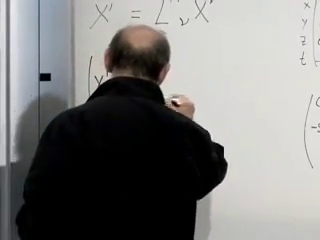
\includegraphics[width=0.8\textwidth]{lecture_06_figure_03.png}
\caption{Các thành phần phản biến và hiệp biến, ma trận metric, và phần mở đầu của phép co bất biến.}
\lectureframe{00:45:00}
\end{figure}

Hạ chỉ số không phải là trang trí. Nó gói gọn các dấu cần thiết cho chuẩn bất biến Lorentz:
\begin{align}
  A_\mu A^\mu
  &=-(A^1)^2-(A^2)^2-(A^3)^2+(A^0)^2,                    \label{eq:l6-norm}\\
  X_\mu X^\mu
  &=t^2-x^2-y^2-z^2.
\end{align}
Biểu thức thứ hai là khoảng không-thời gian bất biến tính từ gốc. Vì \(A^\mu\) biến đổi theo cùng cách như \(X^\mu\), phép co của nó cũng có cùng tính bất biến.

Ký pháp ấy cũng dạy một quy tắc ghi chép hữu ích. Một chỉ số lấy tổng lặp lại xuất hiện một lần ở trên và một lần ở dưới. Ví dụ,
\begin{equation}
  A_\mu A^\mu
  =\eta_{\mu\nu}A^\mu A^\nu.
\end{equation}
Tên của các chỉ số được lấy tổng, hay chỉ số giả, có thể thay đổi mà không làm thay đổi đại lượng.

\begin{classroomqa}
\audiencequestion{Có nên xem một trong các vectơ này là một hàng và cái kia là một cột không, và thứ tự của chúng có quan trọng không?}
\lecturerresponse{Đối với phép tính hiện tại, hãy xem các đại lượng có chỉ số là các thành phần và để metric thực hiện phép co; không cần biến cuộc thảo luận thành đại số toán tử hàng-đối-cột. Đây là các số thông thường, nên thứ tự của chúng không quan trọng. Các toán tử không giao hoán sẽ đòi hỏi cẩn thận hơn, nhưng đó không phải là chủ đề ở đây.}
\end{classroomqa}

Cùng phép xây dựng ấy cho một tích trong giữa hai bốn-vectơ khác nhau,
\begin{equation}
  A\mathbin{\cdot}B=A_\mu B^\mu=A^\mu B_\mu.
\end{equation}
Tính bất biến của nó suy ra mà không cần viết ra một ma trận Lorentz tường minh. Vì \(A+B\) và \(A-B\) là các bốn-vectơ, nên cả hai chuẩn bình phương của chúng đều bất biến:
\begin{align}
  (A+B)^2&=A^2+B^2+2A\mathbin{\cdot}B,\\
  (A-B)^2&=A^2+B^2-2A\mathbin{\cdot}B.
\end{align}
Lấy hiệu cho ta
\begin{equation}
  (A+B)^2-(A-B)^2=4A\mathbin{\cdot}B,                    \label{eq:l6-polarization}
\end{equation}
vì thế \(A\mathbin{\cdot}B\) cũng bất biến. Hệ số 4 suy ra trực tiếp từ phép khai triển.\editorialnote{Lập luận trên bảng cung cấp đồng nhất thức phân cực này; việc viết ra hệ số ấy làm cho phép triệt tiêu được nói bằng lời trở nên không mơ hồ.}

\begin{figure}[H]
\centering
\includegraphics[width=0.8\textwidth]{lecture_06_figure_04.png}
\caption{Hai bình phương bất biến được dùng để tách ra tích trong của hai bốn-vectơ khác nhau.}
\lectureframe{00:52:20}
\end{figure}

Các đại lượng bất biến là những thành phần tự nhiên của các định luật vật lý: khác với một thành phần riêng lẻ, chúng mang cùng một giá trị từ hệ quy chiếu này sang hệ quy chiếu khác.

\section{Vận tốc riêng và bốn-động lượng}

Xét hai sự kiện lân cận trên đường thế giới của một hạt. Độ tách của chúng là vi phân bốn-vectơ
\begin{equation}
  dX^\mu=(dx,dy,dz,dt).
\end{equation}
Với một đường thế giới loại thời, thời gian riêng được định nghĩa bởi
\begin{equation}
  d\tau^2=dX_\mu dX^\mu
  =dt^2-dx^2-dy^2-dz^2.                                  \label{eq:l6-proper-time}
\end{equation}
Bốn-vận tốc riêng là
\begin{equation}
  U^\mu=\frac{dX^\mu}{d\tau}.                            \label{eq:l6-four-velocity}
\end{equation}
Nó đo tốc độ biến thiên của vị trí không-thời gian theo thời gian riêng của chính hạt, chứ không theo thời gian tọa độ của một hệ quy chiếu được chọn.

Mặc dù \(U^\mu\) có bốn thành phần, chỉ có ba trong số đó là độc lập. Chia phương trình~\eqref{eq:l6-proper-time} cho \(d\tau^2\) ta được
\begin{equation}
  U_\mu U^\mu=1.
\end{equation}
Do đó bốn-vận tốc là một vectơ loại thời đơn vị. Việc chọn hướng về tương lai cố định dấu của thành phần thời gian của nó.

\begin{classroomqa}
\audiencequestion{Ở các tốc độ nhỏ hơn rất nhiều so với \(c\), bốn-vận tốc có suy biến thành vận tốc thông thường không?}
\lecturerresponse{Ba thành phần không gian của nó tiến tới vận tốc thông thường, còn thành phần thời gian của nó tiến tới một theo đơn vị \(c=1\). Hệ thức ấy suy ra bằng cách áp dụng quy tắc chuỗi và tính \(dt/d\tau\).}
\end{classroomqa}

Đối với mỗi thành phần không gian,
\begin{equation}
  U^i=\frac{dx^i}{d\tau}
     =\frac{dx^i}{dt}\frac{dt}{d\tau}
     =v^i\frac{dt}{d\tau}.
\end{equation}
Hãy chia phương trình~\eqref{eq:l6-proper-time} cho \(dt^2\):
\begin{equation}
  \left(\frac{d\tau}{dt}\right)^2
  =1-v_x^2-v_y^2-v_z^2
  =1-\boldsymbol v^2.
\end{equation}
Vì thế
\begin{equation}
  \frac{dt}{d\tau}=\frac{1}{\sqrt{1-\boldsymbol v^2}}
  =\gamma(\lvert\boldsymbol v\rvert),
\end{equation}
và
\begin{equation}
  U^\mu=(\gamma v_x,\gamma v_y,\gamma v_z,\gamma).
                                                                  \label{eq:l6-u-components}
\end{equation}

\begin{figure}[H]
\centering
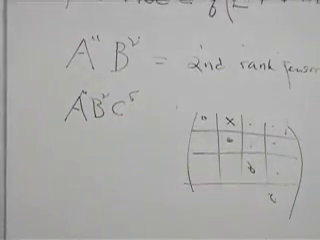
\includegraphics[width=0.8\textwidth]{lecture_06_figure_05.png}
\caption{Phép tính thời gian riêng cho ra \(dt/d\tau=\gamma\) và liên hệ vận tốc riêng với vận tốc thông thường.}
\lectureframe{01:02:00}
\end{figure}

\begin{classroomqa}
\audiencequestion{Liệu \(dx^2/dt^2\) có nghĩa là đạo hàm bậc hai không, và việc bình phương một vectơ có nên sinh ra các hạng chéo không?}
\lecturerresponse{Ở đây nó có nghĩa là \((dx/dt)^2\), tức bình phương của một đạo hàm bậc nhất. Hơn nữa, \(\boldsymbol v^2\) có nghĩa là tích vô hướng Euclid \(v_x^2+v_y^2+v_z^2\), chứ không phải bình phương của tổng hình thức \(v_x+v_y+v_z\); không có các hạng chéo.}
\end{classroomqa}

\begin{classroomqa}
\audiencequestion{Trong \(\gamma(v)\), \(v\) là tốc độ tương đối giữa hai hệ quy chiếu hay là tốc độ của hạt?}
\lecturerresponse{Ở đây, đó là tốc độ của hạt trong hệ quy chiếu đã chọn. Hàm \(\gamma(v)=1/\sqrt{1-v^2}\) có thể được tính cho bất kỳ tốc độ nào: trong một phép biến đổi boost, nó được tính tại tốc độ tương đối của các hệ quy chiếu; còn trong bốn-vận tốc, nó được tính tại tốc độ của hạt.}
\end{classroomqa}

Với \(v\ll1\), \(\gamma\simeq1\), nên các thành phần không gian của \(U^\mu\) tiến tới \(\boldsymbol v\) và \(U^0\) tiến tới một. Khi tốc độ thông thường tiến gần tới tốc độ ánh sáng, \(\gamma\) và mọi thành phần khác không của bốn-vận tốc đều tăng vô hạn.

\begin{classroomqa}
\audiencequestion{Không phải \(U^0\) nên có đơn vị của vận tốc thay vì gần bằng số 1 sao?}
\lecturerresponse{Các đơn vị biến mất khi đặt \(c\) bằng 1. Với \(X^0=ct\), ta có
\(U^\mu=(\gamma\boldsymbol v,\gamma c)\), nên thành phần thời gian tiến tới
\(c\) và \(U_\mu U^\mu=c^2\).}
\end{classroomqa}

Đối với một hạt có khối lượng nghỉ \(m\), định nghĩa bốn-động lượng bởi
\begin{equation}
  P^\mu=mU^\mu.
\end{equation}
Trong đơn vị tự nhiên,
\begin{equation}
  P^\mu=(\gamma m\boldsymbol v,\gamma m).
\end{equation}
Ba thành phần đầu tiên tiến tới động lượng Newton \(m\boldsymbol v\) ở tốc độ thấp. Khôi phục đơn vị, ta được
\begin{equation}
  P^\mu=(\gamma m\boldsymbol v,E/c),
  \qquad E=\gamma mc^2,
\end{equation}
và do đó
\begin{equation}
  E=mc^2+\frac{1}{2}m\boldsymbol v^2+O(mv^4/c^2).
\end{equation}
Thành phần thời gian là năng lượng trong đơn vị \(c=1\), hoặc là năng lượng chia cho \(c\) khi cả bốn thành phần đều được gán đơn vị động lượng.

\begin{classroomqa}
\audiencequestion{Liệu \(\boldsymbol v\) thông thường, với một thành phần thứ tư được thêm vào, tự nó có phải là một bốn-véc-tơ không?}
\lecturerresponse{Không. Ba-vận tốc thông thường không biến đổi như một bốn-véc-tơ. Thừa số \(\gamma\) và định nghĩa theo thời gian riêng là thiết yếu; bốn-véc-tơ là \(U^\mu\), không phải \(\boldsymbol v\).}
\end{classroomqa}

\section{Vì sao điện trường và từ trường phải trộn lẫn}

Bây giờ ta tạm nghỉ ngắn khỏi thuyết tương đối, như vừa nói. Hãy bắt đầu với phương trình chuyển động trước Einstein và hỏi xem nó phải được tổ chức lại như thế nào thì mới có thể đúng trong mọi hệ quán tính. Gia tốc thông thường là đạo hàm theo thời gian của vận tốc thông thường. Tương tự bốn chiều của nó một cách tự nhiên là
\begin{equation}
  A^\mu=\frac{dU^\mu}{d\tau}.
\end{equation}
Ở tốc độ thấp, các thành phần không gian của nó tiến tới gia tốc thông thường. Phương trình tương đối tính đầy đủ sẽ được để lại sau; trước hết hãy xét luật lực cũ.

Đối với một điện tích \(q\) trong điện trường và từ trường,
\begin{equation}
  \boldsymbol F=m\boldsymbol a
  =q\left(\boldsymbol E+\boldsymbol v\times\boldsymbol B\right).
                                                                  \label{eq:l6-lorentz-force}
\end{equation}
Hạng điện không phụ thuộc vào vận tốc của hạt, còn hạng từ thì có phụ thuộc.

\begin{figure}[H]
\centering
\includegraphics[width=0.8\textwidth]{lecture_06_figure_06.png}
\caption{Dạng tiền tương đối tính của định luật lực Lorentz, gợi ý việc kết hợp \(\boldsymbol E\) và \(\boldsymbol B\).}
\lectureframe{01:18:20}
\end{figure}

Giả sử một quan sát viên không thấy điện trường nhưng lại thấy từ trường và một điện tích đang chuyển động. Điện tích ấy chịu một lực từ. Tuy nhiên, trong hệ quy chiếu nghỉ tức thời của điện tích, \(\boldsymbol v=0\), nên số hạng từ trong phương trình~\eqref{eq:l6-lorentz-force} triệt tiêu. Đường thế giới vật lý không trở thành quán tính chỉ vì tọa độ đã thay đổi; vì vậy lực trong hệ mới phải bao gồm một thành phần điện. Nói chính xác hơn, không thể biến đổi một bốn-gia tốc khác không thành bằng không chỉ bằng cách đổi hệ quy chiếu quán tính, mặc dù gia tốc ba chiều và các thành phần của nó quả thật có biến đổi. \editorialnote{Mệnh đề về bốn-gia tốc này là dạng bất biến của lập luận quen thuộc trên lớp học và tránh coi chính gia tốc ba chiều thông thường là bất biến theo hệ quy chiếu.}

Do đó, điện trường và từ trường phải biến đổi thành nhau. Gộp lại, chúng có 6 thành phần, nên chúng không phải là một vô hướng cũng không phải là một bốn-véc-tơ. Ta cần một đối tượng biến đổi mới.

\section{Tensor: mỗi chỉ số ứng với một phép biến đổi}

Một đại lượng vô hướng có thể được gọi là tensor hạng 0; nó không có chỉ số. Một bốn-véc-tơ là tensor hạng 1; nó có một chỉ số với 4 giá trị có thể có. Ví dụ đơn giản nhất về hạng 2 là tích
\begin{equation}
  A^\mu B^\nu.
\end{equation}
Mỗi chỉ số có 4 giá trị, nên đối tượng này có \(4^2=16\) thành phần, có thể được biểu diễn thành một mảng \(4\times4\). Tích của ba véc-tơ,
\begin{equation}
  A^\mu B^\nu C^\sigma,
\end{equation}
có \(4^3=64\) thành phần và là một tensor hạng 3. Các hạng cao hơn tiếp tục theo mẫu đó. Tên gọi kém quan trọng hơn quy tắc xác định đối tượng.

Nếu
\begin{equation}
  A'^{\mu}=\Lambda^\mu{}_{\nu}A^\nu,
  \qquad
  B'^{\sigma}=\Lambda^\sigma{}_{\tau}B^\tau,
\end{equation}
thì tích của chúng biến đổi theo
\begin{equation}
  A'^{\mu}B'^{\sigma}
  =\Lambda^\mu{}_{\nu}\Lambda^\sigma{}_{\tau}
   A^\nu B^\tau.
\end{equation}
Điều này cho ta định luật định nghĩa cho một tensor phản biến hạng 2:
\begin{equation}
  T'^{\mu\sigma}
  =\Lambda^\mu{}_{\nu}\Lambda^\sigma{}_{\tau}T^{\nu\tau}.
                                                                  \label{eq:l6-tensor-transform}
\end{equation}
Có một ma trận Lorentz cho mỗi chỉ số. Các chỉ số lặp \(\nu\) và \(\tau\) được lấy tổng; các chỉ số tự do \(\mu\) và \(\sigma\) ghi nhãn thành phần đang được tính trong hệ có dấu phẩy.

\begin{figure}[H]
\centering
\includegraphics[width=0.82\textwidth]{lecture_06_figure_07.png}
\caption{Phép biến đổi của hai véc-tơ và hệ quả là định luật biến đổi với hai ma trận cho một tensor hạng 2.}
\lectureframe{01:27:15}
\end{figure}

Một tensor không nhất thiết phải là một tích đơn lẻ của các véc-tơ. Cả \(A^\mu B^\nu\) và \(A^\nu B^\mu\) đều tuân theo định luật biến đổi tensor, cũng như tổng của chúng và mọi tổng như
\begin{equation}
  A^\mu B^\nu+C^\mu D^\nu.
\end{equation}
Chính định luật biến đổi, chứ không phải một cách phân tích thừa số cụ thể, mới là định nghĩa. Một tensor hạng 3 nhận thêm ma trận Lorentz thứ ba, và cứ thế tiếp tục.

\section{Tensor đối xứng và phản đối xứng}

Hai lớp tensor hạng 2 sẽ đặc biệt hữu ích. Một tensor đối xứng thỏa mãn
\begin{equation}
  T^{\mu\nu}=T^{\nu\mu},
\end{equation}
nên các phần tử đối xứng qua đường chéo là như nhau. 4 phần tử trên đường chéo và 6 phần tử ở một phía của đường chéo xác định phần còn lại, cho
\begin{equation}
  4+6=10
\end{equation}
thành phần độc lập.

Một tensor phản đối xứng thỏa mãn
\begin{equation}
  T^{\mu\nu}=-T^{\nu\mu}.                                \label{eq:l6-antisymmetry}
\end{equation}
Thay \(\mu=\nu\) vào phương trình~\eqref{eq:l6-antisymmetry} thì được
\(T^{\mu\mu}=-T^{\mu\mu}\), nên mọi phần tử trên đường chéo đều triệt tiêu. 6 phần tử trong một nửa tam giác xác định 6 phần tử kia qua đổi dấu. Vì vậy có đúng 6 thành phần độc lập.

\begin{figure}[H]
\centering
\includegraphics[width=0.82\textwidth]{lecture_06_figure_08.png}
\caption{Một mảng \(4\times4\) phản đối xứng hoàn chỉnh: các số 0 trên đường chéo và các dấu đối nhau qua nó.}
\lectureframe{01:34:25}
\end{figure}

Chính cách đếm đó là đầu mối. 3 thành phần điện và 3 thành phần từ có thể đặt gọn trong một tensor phản đối xứng hạng 2.

\section{Tensor trường điện từ}

Hãy cho các nhãn không-thời gian chạy theo các hàng và cột theo thứ tự
\((1,2,3,0)=(x,y,z,t)\). Cách sắp xếp được viết trên bảng là
\begin{equation}
  F_{\mu\nu}=
  \begin{pmatrix}
    0    & -B_3 & B_2  & E_1\\
    B_3  & 0    & -B_1 & E_2\\
    -B_2 & B_1  & 0    & E_3\\
    -E_1 & -E_2 & -E_3 & 0
  \end{pmatrix}.                                         \label{eq:l6-field-tensor}
\end{equation}
Các ô thuần không gian chứa từ trường; các ô mang một chỉ số không gian và một chỉ số thời gian chứa điện trường. Tính phản đối xứng cho các phần tử tam giác dưới một khi đã biết các phần tử tam giác trên.

\begin{classroomqa}
\audiencequestion{Các phần tử từ có phải đều âm không, và các nhãn có tương ứng với \(x,y,z\) không?}
\lecturerresponse{Các dấu trong tam giác không gian phía trên luân phiên như đã chỉ ra:
\(-B_3,+B_2,-B_1\). Các nhãn \(1,2,3\) tương ứng với \(x,y,z\), còn
\(0\) gắn với thời gian. Phản xạ qua đường chéo đảo mọi dấu.}
\end{classroomqa}

\begin{figure}[H]
\centering
\includegraphics[width=0.82\textwidth]{lecture_06_figure_09.png}
\caption{Tensor trường điện từ hoàn chỉnh theo thứ tự thành phần lấy không gian trước của bài giảng.}
\lectureframe{01:41:05}
\end{figure}

Ký hiệu theo quy ước là \(F_{\mu\nu}\), chứ không phải một \(T_{\mu\nu}\) tổng quát. Giảng viên phỏng đoán rằng chữ cái ấy có thể ám chỉ Faraday, đồng thời nói rõ rằng ông không biết lịch sử của ký hiệu đó. Điều quan trọng ở đây là tính phản đối xứng của nó và 6 thành phần trường của nó, chứ không phải phỏng đoán ấy về chữ cái.

\begin{classroomqa}
\audiencequestion{Mỗi phần tử của ma trận có biểu diễn độ mạnh của một trường trong mặt phẳng tọa độ được chỉ ra không?}
\lecturerresponse{Đó là một thành phần của tensor trường điện từ. Các phần tử liên quan đến thời gian là các thành phần điện, còn các phần tử không gian--không gian mã hóa các thành phần từ.}
\end{classroomqa}

Hãy tách riêng hàng và cột mang chỉ số thời gian. Khối phản đối xứng \(3\times3\) còn lại là phần từ. Có thể nhớ các phần tử độc lập của nó theo chu kỳ:
\begin{equation}
  F_{12}=-B_3,
  \qquad F_{23}=-B_1,
  \qquad F_{31}=-B_2.                                   \label{eq:l6-magnetic-cycle}
\end{equation}
Bắt đầu từ hệ thức đầu tiên, dịch mọi nhãn theo vòng
\(1\to2\to3\to1\). Tương đương,
\begin{equation}
  F_{ij}=-\epsilon_{ijk}B_k,
\end{equation}
với \(\epsilon_{123}=+1\).\editorialnote{Công thức Levi--Civita là dạng chuẩn gọn của quy tắc tuần hoàn đã được triển khai tường minh trên bảng.}

\begin{figure}[H]
\centering
\includegraphics[width=0.82\textwidth]{lecture_06_figure_10.png}
\caption{Các thành phần không gian theo chu kỳ mã hóa từ trường trong tensor phản đối xứng.}
\lectureframe{01:46:20}
\end{figure}

Việc nhận dạng các thành phần điện thì trực tiếp hơn:
\begin{equation}
  E_1=F_{10},
  \qquad E_2=F_{20},
  \qquad E_3=F_{30}.
\end{equation}

Do đó, từ trường có hai cách đồng nhất hữu ích. Trong không gian ba chiều, một véc-tơ trục ba thành phần có thể được ghép cặp với một tensor phản đối xứng \(3\times3\). Tuy nhiên, trong không-thời gian, nó chỉ là phần không gian của tensor 6 thành phần \(F_{\mu\nu}\). Sự ghép cặp này là đặc biệt cho 3 chiều: một tensor phản đối xứng \(4\times4\) có 6 thành phần độc lập và không thể được đồng nhất với một bốn-véc-tơ.
\editorialnote{Dưới các phép quay đúng, từ trường ứng xử như một véc-tơ; dưới các phép phản xạ, chính xác hơn nó là một véc-tơ trục, hay giả véc-tơ.}

Mục đích của phép xây dựng này không phải là đếm thành phần chỉ vì bản thân việc đó. Vì \(F_{\mu\nu}\) biến đổi như một tensor, một phép boost Lorentz tự động trộn các phần tử điện và từ của nó. Trong bài giảng tiếp theo, nó có thể được kết hợp với bốn-vận tốc và bốn-gia tốc để thay phương trình~\eqref{eq:l6-lorentz-force} bằng một phương trình chuyển động hiệp biến.

\section{Các câu hỏi về Einstein và Minkowski}

Những phút cuối chuyển từ phần hình thức sang cách nó nảy sinh trong lịch sử. Các câu trả lời được đưa ra như những hồi tưởng hơn là một lịch sử đã được xác lập, và chính sự bảo lưu đó là một phần của cuộc trao đổi.

\begin{classroomqa}
\audiencequestion{Einstein tìm kiếm một cách phát biểu bất biến Lorentz vì lý do khái niệm, hay ông bị thúc đẩy bởi những quan sát cụ thể?}
\lecturerresponse{Nguyên lý rằng các định luật tự nhiên phải có cùng dạng trong mọi hệ quán tính là trung tâm trong lập luận của ông. Cũng có bằng chứng thực nghiệm liên quan đến ánh sáng và sự thất bại trong việc phát hiện chuyển động qua một ête, mặc dù giảng viên nói rõ rằng ông không chắc Einstein biết những kết quả nào hoặc chúng ảnh hưởng đến ông mạnh đến mức nào. Sức ép về mặt khái niệm là các phương trình Maxwell và lực Lorentz phải tuân theo nguyên lý tương đối, điều này đòi hỏi điện trường, từ trường và các thành phần vận tốc phải cùng biến đổi.}
\end{classroomqa}

Trình bày năm 1905 của Einstein không dùng ký pháp bốn-véc-tơ gọn như ở đây. Nó làm việc theo từng thành phần, với các thừa số cần thiết của \(\gamma\) và vận tốc được viết tường minh. Sau đó Minkowski tổ chức cùng một cấu trúc ấy về mặt hình học như không-thời gian bốn chiều.

\begin{classroomqa}
\audiencequestion{Einstein có chống lại cách phát biểu không-thời gian của Minkowski không, và Minkowski đã đưa nó ra sớm đến mức nào?}
\lecturerresponse{Hồi ức được nêu trong lớp là Einstein ban đầu không đón nhận ngôn ngữ hình học bốn chiều nhưng nhanh chóng chấp nhận giá trị của nó. Mốc thời gian được nêu một cách dè dặt là vào khoảng 2 năm sau bài báo 1905, có lẽ là 1907; người nói nhấn mạnh rằng ông đang hồi tưởng chứ không phải xác lập lịch sử.}
\end{classroomqa}

\begin{classroomqa}
\audiencequestion{Minkowski là nhà toán học hay nhà vật lý, ông còn đóng góp gì khác, và ông có chịu ảnh hưởng của Lorentz hay FitzGerald không?}
\lecturerresponse{Không có câu trả lời chắc chắn nào được khẳng định. Sự phân biệt giữa nhà toán học và nhà vật lý không được theo đuổi đến cùng, một sự đính chính từ khán giả ngắt lời một nhận xét khái quát về công trình khác của Minkowski, và các tuyến ảnh hưởng khả dĩ được để ngỏ một cách minh nhiên. Điểm chắc chắn cho cuộc thảo luận này là vai trò quyết định của Minkowski trong việc tổ chức thuyết tương đối bằng ký pháp hình học bốn chiều.}
\end{classroomqa}

\begin{classroomqa}
\audiencequestion{Các phép biến đổi trộn \(\boldsymbol E\) và
\(\boldsymbol B\) đã có sẵn trong công trình 1905 của Einstein chưa?}
\lecturerresponse{Có, nhưng được viết theo từng thành phần chứ không phải như một phương trình tensor trường duy nhất. Sự so sánh được nêu trong lớp là với các phương trình thành phần của Maxwell: nội dung có thể đã hiện diện trước cả ký pháp gọn làm lộ ra cấu trúc chung của nó. Đóng góp của Minkowski là làm cho cấu trúc ấy trở nên có hệ thống trong ngôn ngữ không-thời gian.}
\end{classroomqa}

Điều đó đưa ta trở lại điểm toán học mà từ đó ta đã bắt đầu. Các thành phần là không thể thiếu cho việc tính toán, nhưng định luật trở nên sáng tỏ khi các thành phần ấy được nhận ra là những phần của một đối tượng duy nhất biến đổi. Nhiệm vụ tiếp theo là dùng \(F_{\mu\nu}\) để viết phương trình chuyển động của hạt mang điện dưới một dạng có cùng hình thức trong mọi hệ quy chiếu quán tính.

\chapter{Hạt tích điện, các phép biến đổi trường và sóng tương đối tính}

Lần trước chúng ta bắt đầu đặt câu hỏi về cách một hạt tích điện chuyển động trong điện trường và từ trường khi các nguyên lý của thuyết tương đối được áp đặt. Định luật lực Lorentz quen thuộc đã chứa sẵn đầu mối: hạng từ của nó phụ thuộc vào vận tốc của hạt, nên các quan sát viên khác nhau không thể tách riêng mà nhất trí với nhau về cái gì là điện và cái gì là từ. Nhiệm vụ của chúng ta là phát biểu định luật ấy sao cho mọi quan sát viên quán tính đều dùng cùng một phương trình, dù các trường và vận tốc của hạt thay đổi từ hệ quy chiếu này sang hệ quy chiếu khác.

Trừ khi có nói khác, chúng ta dùng đơn vị trong đó \(c=1\) và chữ ký metric là \((-,-,-,+)\). Các thành phần không-thời gian được sắp theo thứ tự với 3 thành phần không gian đứng trước:
\begin{equation}
  \mu=(1,2,3,0)=(x,y,z,t).
\end{equation}
Các chỉ số Latin \(m,n\) chỉ chạy trên 3 phương không gian.

\section{Điều gì còn lại của định luật lực Newton}

Trong cơ học Newton,
\begin{equation}
  \boldsymbol F=m\boldsymbol a
\end{equation}
có cùng dạng trong mọi hệ quy chiếu quán tính vì các quan sát viên Galilei đều thống nhất về gia tốc. Họ cũng gán cho hạt cùng một khối lượng và cùng một lực. Khi động học đã thay đổi, không có lý do gì để kỳ vọng quan hệ cụ thể này giữa lực và gia tốc thông thường sẽ còn nguyên vẹn.

Điện từ học và hấp dẫn đã cảnh báo rằng các mở rộng tương đối tính không nhất thiết phải giống nhau. Định luật Coulomb và định luật hấp dẫn Newton đều là các định luật nghịch đảo bình phương, nhưng hấp dẫn không thể được kết hợp một cách tự nhiên vào thuyết tương đối hẹp nếu không có một thay đổi sâu sắc hơn trong hình học không-thời gian. Điện từ học thì có thể. Thật vậy, từ tính bản thân nó là một hiệu ứng tương đối tính: khi khôi phục các thừa số \(c\), một lực từ mang một thừa số vận tốc chia cho \(c\), và nó biến mất trong giới hạn hình thức \(c\to\infty\).

Phần bền vững của định luật Newton là mệnh đề cho rằng lực là tốc độ biến thiên của động lượng. Với khối lượng nghỉ không đổi,
\begin{equation}
  \boldsymbol F
  =m\frac{d\boldsymbol v}{dt}
  =\frac{d}{dt}(m\boldsymbol v)
  =\frac{d\boldsymbol p}{dt}.
\end{equation}
Thuyết tương đối sẽ làm thay đổi quan hệ giữa động lượng và vận tốc, nhưng vẫn bảo toàn cách tổ chức phương trình này.

\begin{figure}[H]
\centering
\includegraphics[width=0.64\textwidth]{lecture_07_figure_01.png}
\caption{Lực được viết lại thành \(d\boldsymbol p/dt\) trong lúc phần điện của định luật Lorentz đang được viết lên bảng.}
\lectureframe{00:08:20}
\end{figure}

Trong đơn vị \(c=1\), định luật lực Lorentz trước tương đối tính là
\begin{equation}
  \frac{d\boldsymbol p}{dt}
  =q\bigl(\boldsymbol E+\boldsymbol v\times\boldsymbol B\bigr).
  \label{eq:lorentz-three}
\end{equation}
Cả hai trường đều có thể phụ thuộc vào vị trí và thời gian. Giới hạn phi tương đối tính bây giờ là giới hạn \(v\ll 1\), chứ không phải một giới hạn mà trong đó hằng số số trị \(c=1\) bằng cách nào đó lại thay đổi. Hạng điện trong \eqref{eq:lorentz-three} vốn đã là một vectơ thông thường. Để hiểu hạng từ dưới một dạng có thể đưa vào không-thời gian, ta phải xem lại tích có hướng.

\section{Tích có hướng như một tensor phản đối xứng}

Xét hai vectơ ba chiều \(\boldsymbol A\) và \(\boldsymbol B\).
Tích ngoài của chúng
\begin{equation}
  T_{mn}=A_mB_n
\end{equation}
là một tenxơ hạng hai với chín thành phần. Nói chung, nó không có đối xứng nào.
Lấy phần phản đối xứng, ta được
\begin{equation}
  K_{mn}=A_mB_n-A_nB_m,
  \qquad K_{mn}=-K_{nm}.
  \label{eq:antisym-product}
\end{equation}
Các phần tử trên đường chéo của nó bằng không, còn mỗi phần tử bên dưới đường chéo được xác định
bởi phần tử tương ứng phía trên nó. Vì vậy, một tenxơ phản đối xứng \(3\times3\)
chỉ có ba thành phần độc lập.

Cách đếm đó gợi ý, nhưng tự nó chưa đủ. 3 đại lượng không tự động biến đổi như một vectơ. Tuy nhiên, trong 3 chiều, 3 phần tử độc lập của \eqref{eq:antisym-product} có thể được đồng nhất với các thành phần của tích có hướng \(\boldsymbol C=\boldsymbol A\times\boldsymbol B\). Trên bảng, \(C_2\) trước hết được đặt tạm vào vị trí góc trên bên phải:

\begin{figure}[H]
\centering
\includegraphics[width=0.75\textwidth]{lecture_07_figure_02.png}
\caption{Tích phản đối xứng trong lúc 3 phần tử độc lập của nó đang được ghép với các thành phần của \(\boldsymbol C\). Nhãn ở góc trên bên phải ở đây vẫn chỉ là tạm thời.}
\lectureframe{00:17:33}
\end{figure}

Cho chu trình \(1\to2\to3\to1\) ta được các công thức thành phần
\begin{align}
  C_3 &= A_1B_2-A_2B_1, \\
  C_1 &= A_2B_3-A_3B_2, \\
  C_2 &= A_3B_1-A_1B_3.
  \label{eq:cross-components}
\end{align}
Dòng cuối cho thấy phần tử ở góc trên bên phải là \(-C_2\), không phải \(C_2\). Sự hiệu chỉnh này là một phần của lập luận chứ không phải là chi tiết cần che đi.

\begin{figure}[H]
\centering
\includegraphics[width=0.62\textwidth]{lecture_07_figure_03.png}
\caption{Các đồng nhất thức thành phần theo chu kỳ đã hoàn chỉnh, dùng để cố định dấu tạm thời trong mảng phản đối xứng.}
\lectureframe{00:21:54}
\end{figure}

Ma trận thu được là
\begin{equation}
  K_{mn}=
  \begin{pmatrix}
    0 & C_3 & -C_2 \\
    -C_3 & 0 & C_1 \\
    C_2 & -C_1 & 0
  \end{pmatrix}.
  \label{eq:cross-matrix}
\end{equation}

Đằng sau ký hiệu này có một hình học hữu ích. Một thành phần mang chỉ số \(1,2\) về tự nhiên gắn với mặt phẳng \(xy\) và được đồng nhất với một thành phần vectơ dọc theo trục vuông góc \(z\). Có thể mô tả cùng một đối tượng có hướng ấy hoặc bằng một mặt phẳng hoặc bằng một mũi tên pháp tuyến với mặt phẳng đó. Cách mô tả bằng mũi tên là đặc thù của 3 chiều; trong các số chiều cao hơn, một tensor phản đối xứng hạng hai vẫn tồn tại, nhưng nó không còn có cùng số thành phần như một vectơ nữa. Vì vậy tensor, chứ không phải mũi tên vuông góc, mới là dạng của tích có hướng có thể tổng quát hóa.

Tương đương, sau khi chọn một định hướng,
\begin{equation}
  C_k=\frac12\epsilon_{kmn}K_{mn}.
\end{equation}
Nhu cầu phải chọn một định hướng là nguồn gốc của quy tắc bàn tay phải và của sự phân biệt quen thuộc giữa vectơ cực và vectơ trục.
\editorialnote{Công thức Levi--Civita và thuật ngữ vectơ trục là ký hiệu chuẩn cho hình học mặt phẳng-đối-với-pháp-tuyến đã được triển khai tường minh trong bài giảng.}

\section{Từ trường dưới dạng tensor}

Mô tả đối ngẫu tương tự cũng áp dụng cho từ trường. Ta định nghĩa tensor không gian phản đối xứng của nó bằng
\begin{equation}
  B_{mn}=
  \begin{pmatrix}
    0 & -B_3 & B_2 \\
    B_3 & 0 & -B_1 \\
    -B_2 & B_1 & 0
  \end{pmatrix}.
  \label{eq:magnetic-tensor}
\end{equation}
Dấu tổng thể phụ thêm so với \eqref{eq:cross-matrix} là một quy ước. Một khi đã chọn, nó phải được dùng nhất quán; nếu đổi dấu của cả 3 thành phần vectơ thì sẽ mô tả cùng một sự đồng nhất giữa tensor và vectơ, nhưng với quy ước định hướng ngược lại.

\begin{figure}[H]
\centering
\includegraphics[width=0.72\textwidth]{lecture_07_figure_04.png}
\caption{Từ trường được viết vừa như một mảng không gian phản đối xứng vừa theo 3 thành phần vectơ của nó.}
\lectureframe{00:24:40}
\end{figure}

Bây giờ lấy thành phần thứ 3 của tích có hướng:
\begin{align}
  (\boldsymbol v\times\boldsymbol B)_3
  &=v_1B_2-v_2B_1 \\
  &=v_1B_{13}+v_2B_{23}+v_3B_{33}.
\end{align}
Có thể thêm hạng cuối vì \(B_{33}=0\). Xoay vòng chỉ số tự do cho ta quy tắc gọn
\begin{equation}
  (\boldsymbol v\times\boldsymbol B)_m=v_nB_{nm},
  \label{eq:cross-contraction}
\end{equation}
trong đó chỉ số lặp \(n\) được lấy tổng. Vì vậy lực từ là
\begin{equation}
  F_m^{(B)}=qv_nB_{nm}.
\end{equation}

\begin{figure}[H]
\centering
\includegraphics[width=0.78\textwidth]{lecture_07_figure_05.png}
\caption{Thành phần thứ 3 của \(\boldsymbol v\times\boldsymbol B\) và biểu thức tổng quát của nó như một phép co với \(B_{nm}\).}
\lectureframe{00:28:30}
\end{figure}

\begin{classroomqa}
\audiencequestion{Chỉ số tự do \(m\) có gắn nhãn cho một thành phần từ riêng biệt của lực không?}
\lecturerresponse{Không. Nó gắn nhãn cho bất cứ thành phần không gian nào của lực đang được tính. Điện trường đơn giản là đã được đặt bằng 0 trong lập luận hiện tại, và ở đây mọi chỉ số chỉ chạy trên 3 phương không gian.}
\end{classroomqa}

Ký hiệu tensor khiến tính chất không sinh công của từ trường gần như trở nên tự động. Lấy đạo hàm của bình phương tốc độ:
\begin{align}
  \frac{d}{dt}(v_mv_m)
  &=2\dot v_m v_m \\
  &\propto 2(\boldsymbol v\times\boldsymbol B)_m v_m \\
  &=2v_nB_{nm}v_m.
  \label{eq:speed-derivative}
\end{align}
Các hạng với \(m=n\) triệt tiêu vì đường chéo của \(B_{nm}\) bằng 0. Mỗi hạng ngoài đường chéo đều có một hạng cặp với \(m\) và \(n\) hoán đổi cho nhau; hai hạng triệt tiêu nhau vì \(v_nv_m\) đối xứng còn \(B_{nm}\) phản đối xứng. Do đó
\begin{equation}
  \frac{d}{dt}(v_mv_m)=0.
\end{equation}
Một lực từ thuần túy bẻ cong quỹ đạo mà không làm thay đổi tốc độ hay động năng của nó.

\begin{figure}[H]
\centering
\includegraphics[width=0.68\textwidth]{lecture_07_figure_06.png}
\caption{Các hạng ghép cặp trong \(v_nB_{nm}v_m\) triệt tiêu vì tensor từ đổi dấu khi hoán đổi các chỉ số của nó.}
\lectureframe{00:35:40}
\end{figure}

Chứng minh này được cố ý trình bày công phu hơn là chỉ nói rằng một tích có hướng vuông góc với thừa số thứ nhất của nó. Mệnh đề sau là điều đặc thù của biểu diễn vectơ 3 chiều. Sự co giữa một cặp đối xứng và một tensor phản đối xứng mới là lập luận sẽ còn tồn tại trong 4 chiều.

\begin{classroomqa}
\audiencequestion{Từ trường có nhất thiết phải độc lập với thời gian để tốc độ giữ không đổi không?}
\lecturerresponse{Phép đại số ở trên không bao giờ lấy đạo hàm trường và không đòi hỏi \(\partial_t\boldsymbol B=0\). Bản thân một hạng từ vẫn không sinh công. Tuy nhiên, trong điện động lực học, một từ trường biến thiên sinh ra một điện trường, và điện trường đó có thể làm thay đổi tốc độ của hạt.}
\end{classroomqa}

\section{Vì sao điện trường và từ trường phải trộn lẫn}

Sự trộn lẫn của \(\boldsymbol E\) và \(\boldsymbol B\) có thể thấy ngay cả trước bất kỳ phép tính 4 chiều nào. Hãy xét chuyển động chậm, để các phát biểu Newton thông thường về gia tốc là đủ dùng. Cho một từ trường hướng dọc theo trục \(y\) và cho một hạt tích điện chuyển động dọc theo trục \(x\). Lực từ hướng dọc theo trục \(z\):
\begin{equation}
  \boldsymbol F=q\boldsymbol v\times\boldsymbol B.
\end{equation}

\begin{figure}[H]
\centering
\includegraphics[width=0.62\textwidth]{lecture_07_figure_07.png}
\caption{Phác họa trên bảng cho một hạt chuyển động ngang qua một từ trường; 3 phương được dùng để so sánh mô tả trong phòng thí nghiệm và mô tả đồng chuyển động.}
\lectureframe{00:42:20}
\end{figure}

Hình học này có thể được vẽ lại mà không cần phối cảnh của lớp học:
\begin{figure}[H]
\centering
\begin{tikzpicture}[scale=1.05,>=Stealth]
  \draw[->] (0,0) -- (3.8,0) node[right] {\(x\)};
  \draw[->] (0,0) -- (-1.9,2.4) node[above left] {\(y\)};
  \draw[->] (0,0) -- (0,3.1) node[above] {\(z\)};
  \draw[->,very thick] (0,0) -- (2.7,0)
    node[midway,below] {\(\boldsymbol v\)};
  \draw[->,very thick] (0,0) -- (-1.35,1.7)
    node[midway,above left] {\(\boldsymbol B\)};
  \draw[->,very thick] (0,0) -- (0,2.35)
    node[midway,right] {\(\boldsymbol F,\ \boldsymbol E'\)};
\end{tikzpicture}
\caption{Trong hệ phòng thí nghiệm, lực hướng \(z\) là lực từ; trong hệ đồng chuyển động tức thời, chính lực ấy phải là lực điện.}
\end{figure}

Giờ hãy xét một quan sát viên đồng chuyển động với hạt tại thời điểm đó. Vận tốc của
hạt trong hệ quy chiếu mới bằng không, nên số hạng từ
\(q\boldsymbol v'\times\boldsymbol B'\) triệt tiêu. Tuy vậy, trong giới hạn chuyển động chậm,
cả hai quan sát viên đều phải nhất trí rằng hạt có gia tốc theo \(z\).
Nếu định luật lực Lorentz có cùng dạng trong cả hai hệ quy chiếu, thì quan sát viên
đồng chuyển động phải quy lực ấy cho một điện trường \(\boldsymbol E'\)
dọc theo \(z\). Vì vậy, một trường thuần từ trong hệ phòng thí nghiệm
không còn thuần từ trong hệ quy chiếu chuyển động.

Đó là lý do vật lý để tìm kiếm một đối tượng duy nhất mà các thành phần của nó bao gồm cả
hai trường. Một phép đổi hệ quy chiếu không chỉ đơn thuần xoay các thành phần của \(\boldsymbol E\) trong
nội bộ ba thành phần riêng của nó và các thành phần của \(\boldsymbol B\) trong nội bộ ba thành phần riêng của nó; nó
trộn lẫn hai bộ đó.

\section{Tensor trường điện từ}

Gộp lại, điện trường và từ trường có 6 thành phần. Một tensor phản đối xứng 4 chiều cũng có 6 thành phần độc lập, vì
\begin{equation}
  \frac{4(4-1)}{2}=6.
\end{equation}
Điều này không có nghĩa rằng một tensor phản đối xứng, theo nghĩa đen, là bộ sưu tập duy nhất gồm 6 đại lượng mà người ta có thể nghĩ ra: 6 vô hướng, hoặc một vectơ và 2 vô hướng, cũng sẽ chứa 6 con số. Nó là đối tượng hình học tự nhiên mà các thành phần của nó có thể trộn lẫn theo cách được đòi hỏi.

Để giữ cho quy ước trên bảng được tường minh, ta hiển thị tensor phản biến theo thứ tự \((1,2,3,0)\), với phần không gian đứng trước:
\begin{equation}
  F^{\mu\nu}=
  \begin{pmatrix}
    0 & -B_3 & B_2 & E_1 \\
    B_3 & 0 & -B_1 & E_2 \\
    -B_2 & B_1 & 0 & E_3 \\
    -E_1 & -E_2 & -E_3 & 0
  \end{pmatrix}.
  \label{eq:l07-field-tensor}
\end{equation}
Khối \(3\times3\) ở góc trên bên trái chính là tensor từ \eqref{eq:magnetic-tensor}; các thành phần có một chỉ số không gian và một chỉ số thời gian chứa điện trường. Tính phản đối xứng cung cấp các phần tử còn lại.

\begin{figure}[H]
\centering
\includegraphics[width=0.72\textwidth]{lecture_07_figure_08.png}
\caption{Khối không gian từ và cột thời gian-không gian điện đang được ghép lại thành tensor trường 4 chiều.}
\lectureframe{00:46:35}
\end{figure}

\begin{classroomqa}
\audiencequestion{Khi nào các thành phần trường này nên mang chỉ số trên thay vì chỉ số dưới?}
\lecturerresponse{Xét riêng 3 nhãn không gian, trên bảng đôi khi người ta lược bỏ sự phân biệt ấy khi nhận diện các trường Maxwell--Faraday quen thuộc. Trong một phép tính hiệp biến, sự phân biệt phải được khôi phục: nâng hoặc hạ một chỉ số không gian sẽ làm đổi dấu trong quy ước metric đã chọn.}
\end{classroomqa}

Điều bất biến không phải là một cách sắp dấu cụ thể nào đó trên bảng, mà là tensor phản đối xứng không-thời gian cùng với một metric nhất quán và một quy ước chỉ số nhất quán. Ký hiệu \(F\) có thể gợi nhớ đến Faraday, mặc dù bài giảng không khẳng định quy gán lịch sử ấy một cách chắc chắn. Einstein đã tìm ra phép biến đổi của các thành phần điện và từ vào 1905; ngôn ngữ tensor 4 chiều cô đọng xuất hiện cùng với cách phát biểu không-thời gian về sau gắn với Minkowski.

\section{Bốn-vận tốc và bốn-lực}

Vế hạt của phương trình cũng phải được viết ở dạng hiệp biến. Thời gian riêng \(\tau\) là bất biến, nên lấy đạo hàm bốn-vectơ vị trí theo nó cho ta một bốn-vectơ khác:
\begin{equation}
  u^\mu=\frac{dx^\mu}{d\tau}
  =\gamma(v_x,v_y,v_z,1),
  \qquad
  \gamma=\frac{1}{\sqrt{1-v^2}}.
  \label{eq:four-velocity}
\end{equation}
Thành phần cuối cùng suy ra từ \(dt/d\tau=\gamma\). Bốn-động lượng là
\begin{equation}
  p^\mu=mu^\mu,
\end{equation}
trong đó phần không gian là động lượng tương đối tính \(\boldsymbol p=m\gamma\boldsymbol v\).

\begin{figure}[H]
\centering
\includegraphics[width=0.75\textwidth]{lecture_07_figure_09.png}
\caption{Bốn-vận tốc, các thành phần của nó, hệ số Lorentz và bốn-động lượng.}
\lectureframe{00:50:30}
\end{figure}

Vì \(p^\mu\) là một bốn-vectơ và \(\tau\) là một đại lượng vô hướng, vế trái tương đối tính tự nhiên là
\begin{equation}
  f^\mu\equiv\frac{dp^\mu}{d\tau}.
  \label{eq:four-force-def}
\end{equation}
Bốn-lực không thể được chọn tùy ý. Bốn-vận tốc có chuẩn cố định,
\begin{equation}
  u_\mu u^\mu=1.
\end{equation}
Lấy đạo hàm dọc theo đường thế cho
\begin{align}
  0
  &=\frac{d}{d\tau}(u_\mu u^\mu) \\
  &=\frac{du_\mu}{d\tau}u^\mu
    +u_\mu\frac{du^\mu}{d\tau} \\
  &=2u_\mu\frac{du^\mu}{d\tau}.
\end{align}
Với khối lượng không đổi, điều này suy ra
\begin{equation}
  f^\mu u_\mu=0.
  \label{eq:force-orthogonal}
\end{equation}
Do đó bốn-lực trực giao theo Minkowski với bốn-vận tốc. Đây là một ràng buộc thuần túy động học hệ quả từ sự chuẩn hóa của \(u^\mu\), chứ không phải là một tính chất đặc biệt của điện từ học.

\begin{figure}[H]
\centering
\includegraphics[width=0.64\textwidth]{lecture_07_figure_10.png}
\caption{Chuẩn đơn vị của bốn-vận tốc và hệ quả là sự trực giao giữa bốn-lực và bốn-vận tốc.}
\lectureframe{00:56:50}
\end{figure}

Phép tính từ trường ba chiều đã cung cấp mẹo để thỏa mãn \eqref{eq:force-orthogonal}. Hãy co một tensor phản đối xứng với một bản sao của vận tốc:
\begin{equation}
  \boxed{
  \frac{dp^\mu}{d\tau}=qF^{\mu\nu}u_\nu.}
  \label{eq:covariant-lorentz}
\end{equation}
Quả thật,
\begin{equation}
  f^\mu u_\mu
  =qF^{\mu\nu}u_\nu u_\mu=0,
\end{equation}
bởi vì \(F^{\mu\nu}\) phản đối xứng còn \(u_\nu u_\mu\) đối xứng.
Đây không phải là định luật lực tương đối tính duy nhất có thể hình dung, nhưng là định luật đơn giản nhất tuyến tính theo cả trường điện từ lẫn vận tốc.

\begin{figure}[H]
\centering
\includegraphics[width=0.72\textwidth]{lecture_07_figure_11.png}
\caption{Phương trình lực Lorentz hiệp biến ở bên trái và phép co bằng không của nó với một bốn-vận tốc thứ hai ở bên phải.}
\lectureframe{01:00:00}
\end{figure}

\section{Khôi phục lực Lorentz thông thường}

Một phương trình mang dáng dấp hiệp biến vẫn phải tái tạo định luật lực đã biết. Với quy ước metric đã nêu ở đầu,
\begin{equation}
  u_\mu=\gamma(-v_x,-v_y,-v_z,1).
\end{equation}
Đối với thành phần \(x\), \eqref{eq:l07-field-tensor} và
\eqref{eq:covariant-lorentz} cho
\begin{align}
  \frac{dp^1}{d\tau}
  &=q\bigl(F^{12}u_2+F^{13}u_3+F^{10}u_0\bigr) \\
  &=q\gamma\bigl(B_3v_y-B_2v_z+E_1\bigr) \\
  &=q\gamma\bigl[\boldsymbol E+\boldsymbol v\times
    \boldsymbol B\bigr]_x.
  \label{eq:x-force}
\end{align}
Các thành phần không gian khác suy ra bằng cách hoán vòng các chỉ số.

\begin{classroomqa}
\audiencequestion{Hạng \(qE_x\) ở đâu trong khai triển theo các thành phần?}
\lecturerresponse{Đó là hạng \(qF^{10}u_0\). Một thành phần của tensor trường có một chỉ số không gian và một chỉ số thời gian chính là một thành phần điện trường, và \(u_0=\gamma\).}
\end{classroomqa}

Thừa số \(\gamma\) ở vế phải không phải là một lực bổ sung. Vì
\begin{equation}
  \frac{dp^i}{d\tau}=\frac{dt}{d\tau}\frac{dp^i}{dt}
  =\gamma\frac{dp^i}{dt},
\end{equation}
nên nó triệt tiêu ở cả hai vế của \eqref{eq:x-force}. Do đó phương trình không gian chính xác lại là
\begin{equation}
  \frac{d\boldsymbol p}{dt}
  =q\bigl(\boldsymbol E+\boldsymbol v\times\boldsymbol B\bigr),
  \qquad
  \boldsymbol p=m\gamma\boldsymbol v.
  \label{eq:exact-three-force}
\end{equation}
Dạng quen thuộc vẫn còn đó, nhưng tính tương đối được ẩn trong động lượng.

\begin{figure}[H]
\centering
\includegraphics[width=0.75\textwidth]{lecture_07_figure_12.png}
\caption{Định luật Lorentz ba chiều được khôi phục sau khi bỏ thừa số thời gian riêng chung; động lượng vẫn giữ thừa số
\(\gamma\).}
\lectureframe{01:06:30}
\end{figure}

Thành phần thời gian mang phát biểu năng lượng tương ứng,
\begin{equation}
  \frac{dp^0}{dt}=q\boldsymbol E\cdot\boldsymbol v,
\end{equation}
vì thế từ trường không thực hiện công, còn điện trường thì có thể làm thay đổi năng lượng của hạt.
\editorialnote{Kiểm tra thành phần thời gian là phần đối ứng trực tiếp với phép tính không gian trong bài giảng; nó được đưa vào để làm lộ ra cùng tính chất không sinh công trong ký hiệu bốn chiều.}

\begin{classroomqa}
\audiencequestion{Phép suy dẫn này là toán học hay vật lý?}
\lecturerresponse{Là cả hai. Đại số tensor cung cấp dạng cô đọng, nhưng đã có vật lý đáng kể được đưa vào thông qua nguyên lý rằng mọi hệ quy chiếu quán tính đều tuân theo cùng những định luật và thông qua giả thiết rằng các phương trình chuyển động là bậc hai. Một định luật bậc hai dự đoán tương lai từ vị trí và vận tốc; một định luật bậc ba sẽ đòi hỏi gia tốc như dữ liệu ban đầu bổ sung. Thí nghiệm, chứ không phải ký hiệu, cho ta biết tự nhiên dùng loại định luật nào.}
\end{classroomqa}

\section{Các trường biến đổi như thế nào}

Phương trình \eqref{eq:covariant-lorentz} có cùng dạng trong mọi hệ quy chiếu vì cả hai vế đều là bốn-vectơ. Bản thân tensor trường biến đổi với một ma trận Lorentz cho mỗi chỉ số:
\begin{equation}
  F'^{\mu\nu}
  =\Lambda^\mu{}_{\rho}\Lambda^\nu{}_{\sigma}F^{\rho\sigma}.
  \label{eq:tensor-transform}
\end{equation}
Trên bảng, quy tắc này được suy ra bằng cách trước hết biến đổi một tích đơn giản
\(A^\mu B^\nu\). Một khi quy tắc đã biết cho tích của các vectơ, tính tuyến tính sẽ cho quy tắc đối với mọi tensor hạng hai.

Đối với một phép boost dọc theo trục \(1\), các tọa độ biến đổi theo
\begin{align}
  x'^1&=\gamma(x^1-vx^0), &
  x'^0&=\gamma(x^0-vx^1), \\
  x'^2&=x^2, & x'^3&=x^3.
\end{align}
Hãy áp dụng cùng phép biến đổi ấy riêng rẽ cho cả hai chỉ số của tensor. Đối với thành phần song song với phép boost, trên bảng bắt đầu từ một tích:
\begin{align}
  (A'^0B'^1)
  =\gamma^2\bigl(
     A^0B^1-vA^0B^0-vA^1B^1+v^2A^1B^0
   \bigr).
\end{align}
Thay từng tích bằng thành phần tensor tương ứng rồi dùng tính phản đối xứng, \(F^{00}=F^{11}=0\) và \(F^{10}=-F^{01}\), ta được
\begin{equation}
  F'^{01}
  =\gamma^2(1-v^2)F^{01}
  =F^{01}.
\end{equation}
Do đó thành phần điện trường song song với chuyển động không đổi. Thành phần từ trường song song cũng ứng xử tương tự.

Các thành phần vuông góc thì khác. Theo quy ước về hệ có dấu phẩy và về dấu được dùng trên bảng,
\begin{align}
  F'^{02}
  &=\gamma\bigl(F^{02}-vF^{12}\bigr), \\
  E'_2
  &=\gamma(E_2+vB_3).
  \label{eq:e-transform}
\end{align}
Một thành phần điện trường vuông góc nhận thêm một phần của một thành phần từ trường. Các định luật biến đổi còn lại tuân theo cùng quy tắc hai chỉ số ấy và được để lại làm bài tập của buổi giảng.

\begin{figure}[H]
\centering
\includegraphics[width=0.76\textwidth]{lecture_07_figure_13.png}
\caption{Phép biến đổi tensor của các thành phần vuông góc tại bước mà thành phần
\(E'_2\) được thấy là chứa một hạng tỉ lệ với \(vB_3\).}
\lectureframe{01:23:40}
\end{figure}

Dấu trong \eqref{eq:e-transform} phụ thuộc vào việc hệ nào được quy ước là chuyển động với \(+v\), cũng như vào các quy ước về chỉ số và metric. Nội dung bất biến của nó thì không: các thành phần điện trường và từ trường vuông góc trộn lẫn nhau, và phương trình lực hiệp biến vẫn còn đúng sau phép biến đổi.

\begin{classroomqa}
\audiencequestion{Đối với dòng điện trong một dây dẫn, liệu ta có thể chuyển động với một vận tốc nào đó để làm cho từ trường triệt tiêu không?}
\lecturerresponse{Chuyển động cùng các electron dẫn là chưa đủ, vì khi đó các điện tích dương của mạng tinh thể lại chuyển động trong hệ quy chiếu mới. Vì vậy, một dây dẫn mang dòng nhưng trung hòa về điện phức tạp hơn trường hợp một khối điện tích đơn lẻ chuyển động. Một từ trường thuần túy không thể bị biến đổi để triệt tiêu hoàn toàn. Nếu cả điện trường lẫn từ trường đều hiện diện, các phần đã biến đổi của chúng có thể triệt tiêu nhau trong những hoàn cảnh đặc biệt; đối với một điện tích chuyển động thẳng đều, hệ nghỉ của điện tích là hệ đơn giản trong đó từ trường của nó triệt tiêu.}
\end{classroomqa}

Phép kiểm tra bất biến chính xác dùng
\begin{equation}
  \boldsymbol B^2-\boldsymbol E^2,
  \qquad
  \boldsymbol E\cdot\boldsymbol B.
\end{equation}
Một hệ quy chiếu với \(\boldsymbol B'=0\) chỉ có thể tồn tại đối với một trường điện trội có \(\boldsymbol E\cdot\boldsymbol B=0\); một trường thuần từ trong một hệ quy chiếu nào đó là từ trội và không thể thỏa điều kiện ấy.
\editorialnote{Các tiêu chuẩn bất biến này phát biểu chính xác điều kiện kèm theo đã đạt tới trong thảo luận trên lớp; phần suy dẫn của chúng được hoãn lại.}

\begin{classroomqa}
\audiencequestion{Thế vô hướng điện và thế vectơ từ có tạo thành một bốn-vectơ không?}
\lecturerresponse{Có. Với các dấu phụ thuộc vào quy ước, chúng gộp lại thành bốn-thế \(A^\mu\). Các phương trình Maxwell sẽ sử dụng một cách có hệ thống đối tượng đó.}
\end{classroomqa}

\section{Đạo hàm của các trường}

Giờ đây ta rời quỹ đạo của một hạt để xét một trường trên toàn bộ không-thời gian. Cho
\begin{equation}
  \phi=\phi(x^1,x^2,x^3,x^0)
\end{equation}
là một trường vô hướng. Bốn đạo hàm của nó tạo thành các thành phần hiệp biến của một bốn-vectơ:
\begin{equation}
  \partial_\mu\phi
  \equiv\frac{\partial\phi}{\partial x^\mu}
  =\left(
    \frac{\partial\phi}{\partial x},
    \frac{\partial\phi}{\partial y},
    \frac{\partial\phi}{\partial z},
    \frac{\partial\phi}{\partial t}
  \right).
\end{equation}
Quy tắc dây chuyền áp dụng cho phép biến đổi tọa độ Lorentz chứng minh định luật biến đổi hiệp biến này. Nâng chỉ số lên làm đảo dấu các thành phần không gian nhưng giữ nguyên dấu của thành phần thời gian:
\begin{equation}
  \partial^\mu\phi
  =\left(
    -\frac{\partial\phi}{\partial x},
    -\frac{\partial\phi}{\partial y},
    -\frac{\partial\phi}{\partial z},
    \frac{\partial\phi}{\partial t}
  \right).
\end{equation}

Mỗi phép lấy đạo hàm đóng góp một chỉ số dưới. Do đó
\(\partial_\nu V^\mu\) là một tensor hạng hai với một chỉ số trên và một chỉ số dưới, còn việc lấy đạo hàm của một tensor tạo ra một đối tượng có thêm một chỉ số dưới. Đây là quy tắc cơ bản cần để viết các phương trình trường mà không phải chọn một hệ quy chiếu quán tính ưu tiên.

\section{Phương trình sóng vô hướng bất biến}

Các phương trình sóng đơn giản nhất chứa hai đạo hàm. Nếu phương trình phải có cùng dạng trong mọi hệ quy chiếu quán tính, thì vế trái của nó nên là một vô hướng. Việc co các chỉ số đạo hàm cho ta lựa chọn đơn giản nhất duy nhất:
\begin{equation}
  \boxed{\partial^\mu\partial_\mu\phi=0.}
  \label{eq:wave-covariant}
\end{equation}
Viết tường minh các thành phần theo quy ước dấu hiện tại,
\begin{equation}
  \frac{\partial^2\phi}{\partial t^2}
  -\frac{\partial^2\phi}{\partial x^2}
  -\frac{\partial^2\phi}{\partial y^2}
  -\frac{\partial^2\phi}{\partial z^2}=0.
  \label{eq:wave-components}
\end{equation}
Phép co trong \eqref{eq:wave-covariant} làm cho tính bất biến Lorentz hiện ra hiển nhiên; phương trình \eqref{eq:wave-components} là cùng phát biểu ấy được viết theo từng thành phần.

\begin{figure}[H]
\centering
\includegraphics[width=0.75\textwidth]{lecture_07_figure_14.png}
\caption{Dạng đạo hàm đã co của phương trình sóng vô hướng và khai triển theo các thành phần thời gian trừ không gian của nó.}
\lectureframe{01:39:40}
\end{figure}

\begin{classroomqa}
\audiencequestion{Vế phải của phương trình sóng có nhất thiết phải bằng không không?}
\lecturerresponse{Không. Nó có thể là bất kỳ vô hướng nào tương thích với bài toán. Một hằng số nhân với \(\phi\), hoặc một hàm vô hướng phi tuyến chẳng hạn tỉ lệ với \(\phi^2\), vẫn bảo toàn tính hiệp biến. Giá trị bằng không cho phương trình sóng tự do đơn giản nhất.}
\end{classroomqa}

Mục đích của ví dụ vô hướng này là để chuẩn bị. Các phương trình Maxwell trộn điện trường và từ trường theo cách phức tạp hơn, nhưng chúng cũng có thể được viết sao cho tính bất biến Lorentz hiện rõ từ cấu trúc chỉ số của chúng. Đó là vấn đề mà lần tới ta sẽ quay lại.

\chapter{Metric, sự giãn nở và vũ trụ học bước đầu}

Ở cuối bài giảng trước, chúng ta đã đi tới một phương trình sóng bất biến Lorentz và đang chuẩn bị viết các phương trình Maxwell dưới dạng không-thời gian. Một câu hỏi từ người nghe giờ đây đưa ra một lời lưu ý hữu ích trước khi chuyển sang hấp dẫn: bản thân đối xứng có thể quyết định được bao nhiêu của một lý thuyết vật lý? Câu trả lời là dứt khoát: rất nhiều, nhưng không phải tất cả. Tính bất biến Lorentz là một bộ lọc mạnh đối với các định luật khả dĩ. Nó không thay thế cho các giả thiết vật lý còn lại hay cho thực nghiệm.

\section{Điều mà đối xứng không quyết định}

\begin{classroomqa}
\audiencequestion{Một khi đã biết điện trường và từ trường cùng biến đổi với nhau dưới các phép biến đổi Lorentz, thì các phương trình Maxwell có suy ra chỉ từ thuyết tương đối hay không?}
\lecturerresponse{Không. Thuyết tương đối ràng buộc dạng của các phương trình, nhưng việc xây dựng còn dùng đến tính tuyến tính của chúng, bậc thấp của các đạo hàm, cách các trường biến đổi, và thông tin thực nghiệm. Nếu thiếu những yếu tố bổ sung ấy thì vẫn còn nhiều phương trình trường hiệp biến Lorentz khác khả dĩ.}
\end{classroomqa}

Giả thiết bổ sung quan trọng nhất cho phần mở đầu ấy là tính tuyến tính. Nếu \(A(x,t)\) là một nghiệm của một phương trình trường tuyến tính, thì \(\lambda A(x,t)\) cũng là một nghiệm với mọi hằng số \(\lambda\). Nếu \(A\) và \(B\) là các nghiệm, thì \begin{equation}
  C(x,t)=A(x,t)+B(x,t).
  \label{eq:superposition}
\end{equation}
Đây là nguyên lý chồng chất. Hai sóng điện từ không nguồn có thể đi xuyên qua nhau rồi đi ra mà không đổi. Chúng không va chạm trực tiếp như các vật chất vẫn làm. Chúng có thể tương tác gián tiếp thông qua vật chất mang điện, vì mỗi sóng làm các điện tích chuyển động và các điện tích chuyển động phát bức xạ, nhưng bản thân các phương trình trường trong chân không là tuyến tính.

\begin{figure}[H]
\centering
\includegraphics[width=0.64\textwidth]{lecture_08_figure_01.png}
\caption{Hai biên dạng sóng trên bảng trong phần thảo luận về nguyên lý chồng chất. Tổng của chúng lại là một sóng không nguồn hợp lệ.}
\lectureframe{00:05:30}
\end{figure}

Dao động điều hòa làm cho đại số trở nên minh bạch. Giả sử
\begin{equation}
  m\ddot x=-kx.
  \label{eq:linear-oscillator}
\end{equation}
Nếu \(x_1\) và \(x_2\) nghiệm \eqref{eq:linear-oscillator}, thì
\begin{equation}
  m(\ddot x_1+\ddot x_2)
  =-k(x_1+x_2),
\end{equation}
nên \(x_1+x_2\) là một nghiệm. Tuy nhiên, nếu thêm một hạng phi tuyến,
\begin{equation}
  m\ddot x=-kx+p x^2,
  \label{eq:nonlinear-oscillator}
\end{equation}
thì tổng không còn dùng được nữa:
\begin{equation}
  (x_1+x_2)^2=x_1^2+x_2^2+2x_1x_2.
\end{equation}
Hạng chéo \(2x_1x_2\) không có hạng tương ứng nào trong hai phương trình riêng rẽ. Hai chuyển động giờ đây ảnh hưởng lẫn nhau.

\begin{figure}[H]
\centering
\includegraphics[width=0.73\textwidth]{lecture_08_figure_02.png}
\caption{Các phương trình dao động riêng rẽ được so sánh với phương trình cho tổng của chúng. Hạng bậc hai làm lộ ra hạng chéo phụ thêm phá vỡ nguyên lý chồng chất.}
\lectureframe{00:10:10}
\end{figure}

Ví dụ này xác lập điểm phương pháp luận sẽ còn hiệu lực trong suốt phần thảo luận về vũ trụ học. Đối xứng cho ta biết những đại lượng nào có thể kết hợp và những phương trình nào được phép. Động lực học và quan sát cho ta biết tự nhiên sử dụng phương trình được phép nào.

\section{Khoảng không-thời gian như hình học}

Bây giờ ta rời điện từ học và đi theo một lối ngắn vào thuyết tương đối rộng và vũ trụ học. Đối tượng xuất phát là khoảng giữa các sự kiện lân cận. Gán cho một sự kiện bốn tọa độ \(x^\mu\) và cho một sự kiện lân cận là \(x^\mu+dx^\mu\). Trong hệ tọa độ Descartes quán tính, với \(c=1\) và quy ước \((+,-,-,-)\),
\begin{equation}
  d\tau^2
  =dt^2-dx^2-dy^2-dz^2
  =dx^\mu dx_\mu
  =\eta_{\mu\nu}\,dx^\mu dx^\nu.
  \label{eq:minkowski-interval}
\end{equation}
Đại lượng bất biến là \(d\tau^2\), chứ không phải bất kỳ độ chênh tọa độ riêng lẻ nào. Các phép biến đổi Lorentz làm thay đổi \(dt,dx,dy,dz\) trong khi vẫn bảo toàn tổ hợp bậc hai này. Vì thế, thuyết tương đối hẹp có thể được đọc như hình học của không-thời gian Minkowski.

\begin{figure}[H]
\centering
\includegraphics[width=0.72\textwidth]{lecture_08_figure_03.png}
\caption{Khoảng Minkowski được viết lần lượt dưới ký hiệu theo thành phần, chỉ số co, và tensor metric.}
\lectureframe{00:14:50}
\end{figure}

Sự đơn giản của \eqref{eq:minkowski-interval} phụ thuộc vào tọa độ. Ngay cả một mặt phẳng cũng có thể mang các hệ số lạ nếu ta gán nhãn nó một cách vụng về. Hãy để \(x\) được đo bằng xentimét, còn \(y\) được đo bằng mét. Đối với một độ dời vật lý,
\begin{equation}
  ds^2=dx^2+\left(\frac{dy}{100}\right)^2
      =dx^2+10^{-4}dy^2.
  \label{eq:mixed-units}
\end{equation}
Hệ số \(10^{-4}\) không nói gì về độ cong. Nó chỉ đơn thuần chuyển đổi giữa các đơn vị.

\begin{figure}[H]
\centering
\includegraphics[width=0.59\textwidth]{lecture_08_figure_04.png}
\caption{Một mặt phẳng được mô tả với xentimét trên một trục và mét trên trục kia. Các hệ số metric không bằng nhau mã hóa đơn vị, chứ không phải độ cong.}
\lectureframe{00:20:10}
\end{figure}

Tọa độ xiên thêm vào một hạng hỗn hợp. Trong hai chiều, dạng toàn phương địa phương tổng quát nhất có thể được viết
\begin{align}
  ds^2
  &=a_{11}\,dx^2+a_{12}\,dx\,dy\notag\\
  &\quad+a_{21}\,dy\,dx+a_{22}\,dy^2,
  \qquad a_{12}=a_{21}.
  \label{eq:quadratic-form}
\end{align}
Vì các vi phân thông thường giao hoán, \(dx\,dy=dy\,dx\), nên chỉ phần đối xứng của mảng hệ số mới đóng góp. Ta gom các hệ số vào ma trận
\begin{equation}
  g=
  \begin{pmatrix}
    a_{11} & a_{12}\\
    a_{21} & a_{22}
  \end{pmatrix}.
  \label{eq:metric-matrix}
\end{equation}
Ma trận này là \emph{metric}. Nó là quy tắc địa phương biến các hiệu tọa độ thành các khoảng vật lý.

\begin{figure}[H]
\centering
\includegraphics[width=0.71\textwidth]{lecture_08_figure_05.png}
\caption{Dạng vi phân toàn phương và ma trận hệ số đối xứng \(2\times2\) của nó tại thời điểm ma trận được nhận diện là metric.}
\lectureframe{00:24:07}
\end{figure}

Các lưới chữ nhật hoặc xiên đồng đều cho các hệ số hằng. Nếu các đường tọa độ cong đi, dồn lại gần nhau hoặc tách xa nhau, thì các hệ số ấy trở thành các hàm của vị trí ngay cả khi mặt nền bên dưới vẫn phẳng. Ký hiệu không-thời gian tổng quát là
\begin{equation}
  ds^2=g_{\mu\nu}(x)\,dx^\mu dx^\nu.
  \label{eq:general-metric}
\end{equation}

\begin{figure}[H]
\centering
\includegraphics[width=0.66\textwidth]{lecture_08_figure_06.png}
\caption{Metric tổng quát phụ thuộc vị trí sau khi cho phép lưới tọa độ biến thiên từ điểm này sang điểm khác.}
\lectureframe{00:28:10}
\end{figure}

Biết \(g_{\mu\nu}\) trong một hệ tọa độ xác định sẽ quyết định các khoảng cách, thời gian và góc địa phương, và do đó quyết định hình học. Chiều ngược lại không đơn nhất: một hình học có vô số mô tả tọa độ, vì thế có vô số mảng hàm hệ số liên hệ với nhau bởi các phép biến đổi tọa độ.

\section{Độ phức tạp tọa độ và độ cong nội tại}

Giờ ta phải phân biệt một metric phức tạp với một không gian cong. Hãy cuộn một tờ giấy thành hình trụ mà không kéo dãn nó. Hình dáng của nó trong căn phòng thay đổi, nhưng mọi khoảng cách đo ngay trong tờ giấy vẫn giữ nguyên. Một sinh vật bị giam trên tờ giấy không thể phát hiện sự uốn đó bằng bất kỳ phép đo nội tại nào. Đó là sự uốn ngoại tại, không phải độ cong được nói đến ở đây.

Một bán cầu thì khác. Nó không thể bị ép phẳng mà không bị kéo dãn, xé rách hoặc nén lại. Một bản đồ phẳng của Trái Đất tất yếu phải làm méo hoặc khoảng cách, hoặc diện tích, hoặc góc, hoặc một tổ hợp nào đó của chúng. Trở ngại này là nội tại và có thể được phát hiện mà không cần nhìn vào một chiều bao quanh.

Tọa độ cực cho phản ví dụ phẳng không thể thiếu. Trên một mặt phẳng, một độ dời xuyên tâm vô cùng nhỏ có độ dài \(dr\), còn một độ dời góc \(d\theta\) tại bán kính \(r\) có độ dài \(r\,d\theta\). Do đó
\begin{equation}
  ds^2=dr^2+r^2d\theta^2,
  \qquad
  g_{\text{polar}}=
  \begin{pmatrix}
    1&0\\
    0&r^2
  \end{pmatrix}.
  \label{eq:polar-metric}
\end{equation}
Hệ số \(r^2\) biến thiên trên khắp mặt phẳng, nhưng mặt phẳng vẫn phẳng. Phép đổi biến
\begin{equation}
  x=r\cos\theta,\qquad y=r\sin\theta
\end{equation}
đưa ta trở lại metric hằng \(ds^2=dx^2+dy^2\).

\begin{figure}[H]
\centering
\includegraphics[width=0.70\textwidth]{lecture_08_figure_07.png}
\caption{Metric cực và sự trở về của nó với metric Descartes. Ma trận phụ thuộc vị trí ở bên trái vẫn mô tả một mặt phẳng.}
\lectureframe{00:39:20}
\end{figure}

\begin{classroomqa}
\audiencequestion{Khoảng cách góc trong tọa độ cực có nên chứa một hàm sine không?}
\lecturerresponse{Không, trên mặt phẳng thì không. Ở đó độ dài cung là \(r\,d\theta\). Một hàm sine xuất hiện trên mặt cầu, nơi một vòng vĩ tuyến có bán kính \(R\sin\theta\).}
\end{classroomqa}

Xét một mặt cầu bán kính \(R\). Gọi \(\theta\) là góc cực đo từ cực bắc và \(\phi\) là góc phương vị. Một bước theo kinh tuyến có độ dài \(R\,d\theta\). Tại góc cực \(\theta\), vòng vĩ tuyến có bán kính \(R\sin\theta\), nên một bước theo phương vị có độ dài
\(R\sin\theta\,d\phi\). Định lý Pythagoras địa phương cho
\begin{align}
  ds^2
  &=R^2\left(d\theta^2+\sin^2\theta\,d\phi^2\right),
  \label{eq:sphere-metric}\\
  g_{\text{sphere}}=
  &\begin{pmatrix}
    R^2&0\\
    0&R^2\sin^2\theta
  \end{pmatrix}.
\end{align}

\begin{figure}[H]
\centering
\includegraphics[width=0.72\textwidth]{lecture_08_figure_08.png}
\caption{Mặt cầu, phần tử độ dài góc của nó, và ma trận metric tương ứng. Thừa số \(\sin^2\theta\) ghi nhận sự co nhỏ dần của các vòng vĩ tuyến.}
\lectureframe{00:45:15}
\end{figure}

\begin{figure}[H]
\centering
\begin{tikzpicture}[scale=1.05]
  \draw (0,0) circle (2.1);
  \draw[dashed] (-2.1,0) arc (180:360:2.1 and 0.52);
  \draw (2.1,0) arc (0:180:2.1 and 0.52);
  \coordinate (P) at (48:2.1);
  \fill (P) circle (1.5pt);
  \draw (0,0) -- (0,2.1);
  \draw (0,0) -- (P);
  \draw (0,0.82) arc (90:48:0.82);
  \node at (0.47,1.03) {\(\theta\)};
  \draw[->] (P) -- ++(-0.34,0.36)
    node[midway,left] {\(R\,d\theta\)};
  \draw[->] (P) -- ++(0.76,0)
    node[midway,above] {\(R\sin\theta\,d\phi\)};
\end{tikzpicture}
\caption{Dựng lại gọn gàng các cạnh vi phân địa phương dùng để thu được \eqref{eq:sphere-metric}.}
\end{figure}

Không có phép đổi tọa độ toàn cục nào biến \eqref{eq:sphere-metric} thành một ma trận Euclid hằng. Một quan sát viên hai chiều có thể phát hiện điều này một cách nội tại: một tam giác đủ lớn ghép từ các đường trắc địa có tổng các góc lớn hơn \(180^\circ\). Vì thế ta đã đạt tới tiêu chuẩn hữu ích. Các hệ số biến thiên tự chúng không hàm ý độ cong. Độ cong là trở ngại đối với việc tìm được các tọa độ làm cho metric hằng trên toàn bộ miền đang xét.

\section{Từ không-thời gian cong đến vũ trụ học}

Thuyết tương đối rộng cho phép chính không-thời gian mang độ cong nội tại này. Một \(g_{\mu\nu}\) phụ thuộc vị trí vẫn có thể chỉ là một tạo tác của tọa độ, như trong tọa độ cực, nhưng trong một không-thời gian thực sự cong thì không có phép biến đổi tọa độ nào loại bỏ được sự biến thiên ấy trên toàn cục.

\begin{figure}[H]
\centering
\includegraphics[width=0.70\textwidth]{lecture_08_figure_09.png}
\caption{Sự chuyển tiếp từ các ví dụ tọa độ đặc biệt sang phần tử độ dài không-thời gian tổng quát \(ds^2=g_{\mu\nu}(x)dx^\mu dx^\nu\).}
\lectureframe{00:48:40}
\end{figure}

Chúng ta sẽ không thử triển khai toàn bộ bộ máy của các phương trình Einstein. Thay vào đó, ta giới hạn sự chú ý vào các hình học thích hợp cho vũ trụ học: không gian được giả thiết là đồng nhất trên các thang đủ lớn, trong khi hình học có thể thay đổi theo thời gian. Đồng nhất có nghĩa là không có vị trí nào được ưu tiên hơn vị trí khác. Nó không có nghĩa là phẳng: mọi điểm trên một mặt cầu đều tương đương, nhưng mặt cầu vẫn cong. Nó cũng không có nghĩa là không có cấu trúc ở mọi thang.

\begin{classroomqa}
\audiencequestion{Làm sao vũ trụ có thể đồng nhất khi các thiên hà tạo thành các cụm, các tấm và các sợi?}
\lecturerresponse{Khẳng định này liên quan tới các thang được làm trơn thô. Các sao, thiên hà và cụm thiên hà là rất không đồng nhất. Khi so sánh các vùng có kích thước hàng trăm triệu năm ánh sáng, những cấu trúc đó được lấy trung bình hướng tới một phân bố đồng đều. Nguyên lý vũ trụ học là một giả thuyết làm việc có tính kinh nghiệm, không phải một tất yếu logic; những sai khác có hệ thống đủ lớn, kể cả các sai khác theo hướng trong nền vũ trụ, có thể bác bỏ nó.}
\end{classroomqa}

Giả thiết thang lớn thứ hai trong bài giảng này là tính phẳng không gian. Tại một thời gian vũ trụ cố định, các tam giác đủ lớn có vẻ Euclid: các góc của chúng cộng lại thành \(180^\circ\). Đây là một phát biểu về hình học của không gian ba chiều, chưa phải về độ cong của không-thời gian bốn chiều.

\begin{classroomqa}
\audiencequestion{Tính đồng thời có nghĩa gì đối với các điểm cách nhau bởi những khoảng cách vũ trụ học, khi ánh sáng từ chúng đến với ta ở các thời điểm khác nhau?}
\lecturerresponse{Chúng ta không thể đặt các thước đo giữa các thiên hà xa xôi hoặc quan sát chúng một cách tức thời. Ta nhận tín hiệu muộn hơn rồi tái dựng hình học của các sự kiện phát xạ trong một mô hình không-thời gian. Quy trình này là gián tiếp, nhưng nhiều phép đo hình học trong thiên văn học cũng vậy. Tính phẳng có nghĩa là các tam giác lớn được tái dựng không cho thấy phần thừa góc hay phần thiếu góc nào có thể phát hiện được trên thang đã khảo sát.}
\end{classroomqa}

\section{Tọa độ đồng chuyển động và thừa số tỉ lệ}

Hãy hình dung một lưới Descartes được vẽ lên dòng chảy thang lớn của các thiên hà. Mỗi thiên hà giữ nguyên nhãn tọa độ của mình khi lưới giãn ra. Nhãn ấy không phải là một khoảng cách tính bằng mét; nó là một địa chỉ. Một thừa số chuyển đổi phụ thuộc thời gian biến các độ tách tọa độ thành các độ tách vật lý.

\begin{figure}[H]
\centering
\begin{tikzpicture}[>=Latex,scale=0.86]
  \foreach \x in {0,0.65,1.3,1.95,2.6} {
    \draw[gray!65] (\x,0) -- (\x,2.2);
  }
  \foreach \y in {0,0.55,1.1,1.65,2.2} {
    \draw[gray!65] (0,\y) -- (2.6,\y);
  }
  \fill[blue!65!black] (0.65,0.55) circle (2pt);
  \fill[red!70!black] (1.95,1.65) circle (2pt);
  \node[below] at (1.3,-0.2) {comoving labels at \(t_1\)};
  \draw[->,very thick] (3.0,1.1) -- (4.0,1.1)
    node[midway,above] {\(a(t)\) grows};
  \foreach \x in {4.4,5.5,6.6,7.7,8.8} {
    \draw[gray!65] (\x,0) -- (\x,2.2);
  }
  \foreach \y in {0,0.55,1.1,1.65,2.2} {
    \draw[gray!65] (4.4,\y) -- (8.8,\y);
  }
  \fill[blue!65!black] (5.5,0.55) circle (2pt);
  \fill[red!70!black] (7.7,1.65) circle (2pt);
  \node[below] at (6.6,-0.2) {same labels at \(t_2\)};
\end{tikzpicture}
\caption{Các địa chỉ đồng chuyển động giữ nguyên, trong khi khoảng cách vật lý của lưới tọa độ tăng lên.}
\end{figure}

Tính đồng nhất không gian đòi hỏi cùng một thừa số chuyển đổi ở mọi nơi tại một thời điểm cho trước. Tính phẳng không gian cho phép phần không gian của metric có dạng Descartes. Phần tử độ dài thu được là
\begin{equation}
  d\tau^2
  =dt^2-a^2(t)\left(dx^2+dy^2+dz^2\right).
  \label{eq:flrw-flat}
\end{equation}
Đây là metric vũ trụ học đồng nhất phẳng theo không gian trong tọa độ đồng chuyển động. Ta có thể chọn \(x,y,z\) không thứ nguyên và cho \(a(t)\) đơn vị độ dài. Một quy ước khác có thể đưa thứ nguyên vào các tọa độ và làm cho \(a\) không thứ nguyên; chỉ tích của chúng mới quan trọng.

\begin{figure}[H]
\centering
\includegraphics[width=0.76\textwidth]{lecture_08_figure_10.png}
\caption{Metric vũ trụ học phẳng theo không gian như đã được hoàn tất trên bảng, với thừa số chung \(a^2(t)\) nhân lên cả ba phương không gian.}
\lectureframe{01:03:15}
\end{figure}

Nếu \(a\) là hằng số, ta có thể hấp thụ nó bằng cách đổi tỷ lệ \(x,y,z\), và \eqref{eq:flrw-flat} sẽ là không-thời gian Minkowski thông thường với các đơn vị khác đi. Sự phụ thuộc theo thời gian của nó mới là thành phần không tầm thường.

\begin{classroomqa}
\audiencequestion{Nếu lưới tọa độ giãn nở, tại sao thước mét, nguyên tử và các thiên hà lại không giãn nở cùng nó?}
\lecturerresponse{Metric mô tả dòng chảy vũ trụ trung bình, không phải một lực buộc mọi hệ liên kết phải đi theo nó. Lực điện từ giữ cho thước mét và nguyên tử kết dính; tự hấp dẫn giữ cho một thiên hà kết dính. Những hiệu ứng liên kết đó lấn át sự giãn nở nền cực kỳ yếu ở các thang nhỏ. Các thiên hà ở gần cũng có thể lệch khỏi dòng Hubble: Andromeda bị kéo về phía Ngân Hà. Các nghiên cứu chi tiết về sự liên kết hấp dẫn của thiên hà cho thấy chỉ riêng vật chất khả kiến là không đủ, đó là một trong những lập luận ủng hộ vật chất tối.}
\end{classroomqa}

\begin{classroomqa}
\audiencequestion{Vì sao thừa số tỉ lệ bản thân nó không phải là một lực đẩy các thiên hà ra xa nhau?}
\lecturerresponse{Theo quy ước hiện tại, nó có thứ nguyên độ dài, chứ không phải lực. Hãy nghĩ đến một viên đạn đại bác được bắn lên cao. Một khi đã được phóng đi, chuyển động hướng ra ngoài của nó là chuyển động quán tính; hấp dẫn làm thay đổi chuyển động đó bằng cách giảm tốc của nó hoặc kéo nó trở lại. Tương tự, sự giãn nở là một trạng thái chuyển động. Câu hỏi động lực học là hấp dẫn và các nguồn khác làm thay đổi \(\dot a\) và \(\ddot a\) như thế nào, chứ không phải cần lực gì để duy trì chuyển động của \(a\).}
\end{classroomqa}

Kỳ vọng trước đây là hấp dẫn hút phải làm chậm sự giãn nở. Đến thời điểm của bài giảng này, bằng chứng thiên văn đã cho thấy thay vào đó sự giãn nở gần đây đang tăng tốc, điều đó có nghĩa là động lực học đầy đủ chứa nhiều hơn vật chất hút thông thường. Ta hoãn vấn đề ấy cho đến khi thiết lập hình học đã vững chắc.

\section{Định luật Hubble}

Lấy hai thiên hà đồng chuyển động có độ tách tọa độ cố định là \(\Delta x\). Tại cùng một thời gian vũ trụ, khoảng cách vật lý của chúng là
\begin{equation}
  D(t)=a(t)\,\Delta x.
  \label{eq:physical-distance}
\end{equation}
Lấy đạo hàm trong khi giữ cố định các nhãn đồng chuyển động:
\begin{align}
  V(t)
    &=\dot D(t)
      =\dot a(t)\,\Delta x \nonumber\\
    &=\frac{\dot a(t)}{a(t)}D(t).
  \label{eq:hubble-derivation}
\end{align}
Định nghĩa
\begin{equation}
  H(t)=\frac{\dot a(t)}{a(t)}.
  \label{eq:hubble-parameter}
\end{equation}
Khi đó
\begin{equation}
  V(t)=H(t)D(t).
  \label{eq:hubble-law}
\end{equation}
Tại một thời gian vũ trụ cho trước, cùng một \(H(t)\) áp dụng ở mọi nơi; nếu không, không gian sẽ không đồng nhất. Vận tốc lùi tỉ lệ với khoảng cách vì mọi khoảng trên lưới đồng chuyển động đều bị kéo giãn với cùng một tốc độ tương đối.

\begin{figure}[H]
\centering
\includegraphics[width=0.73\textwidth]{lecture_08_figure_11.png}
\caption{Khoảng cách vật lý \(D=a\Delta x\) và đạo hàm theo thời gian của nó, trên đường dẫn tới \(V=(\dot a/a)D\).}
\lectureframe{01:16:45}
\end{figure}

\begin{classroomqa}
\audiencequestion{Đối với một thiên hà ở xa, nên lấy giá trị của tham số Hubble ở hiện tại hay tại lúc ánh sáng quan sát được đã được phát ra?}
\lecturerresponse{Tại thời kỳ đang được mô tả. Ánh sáng từ một thiên hà ở xa cho biết một giá trị sớm hơn của sự giãn nở. Một phân tích nghiêm túc phải tính đến sự phụ thuộc theo thời gian của \(H\); việc thay giá trị hôm nay vào mọi nơi chỉ là một xấp xỉ cục bộ.}
\end{classroomqa}

\begin{classroomqa}
\audiencequestion{Các đơn vị nằm ở đâu trong \(D=a\Delta x\)?}
\lecturerresponse{Một lựa chọn thuận tiện là coi nhãn đồng chuyển động \(\Delta x\) là không thứ nguyên và để \(a\) mang thứ nguyên độ dài. Cũng có thể phân bổ đơn vị theo cách ngược lại. Dù theo cách nào, \(H=\dot a/a\) có thứ nguyên nghịch đảo thời gian.}
\end{classroomqa}

\section{Ánh sáng trong hệ tọa độ giãn nở}

Ánh sáng đi theo một quỹ đạo null. Dọc theo một quỹ đạo như vậy, khoảng thời gian riêng bằng không:
\begin{equation}
  d\tau^2=0.
\end{equation}

\begin{classroomqa}
\audiencequestion{Vì sao khoảng này bằng không đối với ánh sáng?}
\lecturerresponse{Đó là hình học định nghĩa của một tia sáng trong thuyết tương đối. Mọi quan sát viên rơi tự do cục bộ đều đo được ánh sáng chuyển động với \(c=1\), nên cục bộ \(dt^2=d\ell^2\) và khoảng không-thời gian bằng không. Điều đó không có nghĩa là không có thời gian tọa độ nào trôi qua đối với quan sát viên nhận ánh sáng.}
\end{classroomqa}

Đối với một tia chỉ chuyển động theo hướng \(x\),
\begin{equation}
  0=dt^2-a^2(t)\,dx^2.
\end{equation}
Chọn tia chuyển động theo chiều \(x\) tăng,
\begin{equation}
  dt=a(t)\,dx,
  \qquad
  dx=\frac{dt}{a(t)},
  \qquad
  \frac{dx}{dt}=\frac{1}{a(t)}.
  \label{eq:null-ray}
\end{equation}

\begin{figure}[H]
\centering
\includegraphics[width=0.64\textwidth]{lecture_08_figure_12.png}
\caption{Điều kiện null trong metric giãn nở và phương trình tia sáng trong tọa độ đồng chuyển động suy ra \(dx=dt/a(t)\).}
\lectureframe{01:23:45}
\end{figure}

Vận tốc tọa độ \(dx/dt\) giảm khi thừa số tỉ lệ tăng. Điều này không có nghĩa là ánh sáng chậm đi một cách cục bộ. Một đơn vị khoảng cách tọa độ đồng chuyển động biểu diễn một khoảng cách vật lý ngày càng lớn hơn, nên giá trị số của vận tốc tọa độ thay đổi trong khi mọi phép đo cục bộ vẫn cho \(c=1\).

\section{Vì sao sự phụ thuộc theo thời gian lại quan trọng}

Câu hỏi hình học trung tâm giờ đây không thể né tránh: \(a(t)\) biến thiên như thế nào? Phép tương tự là một vật phóng mà ta biết vị trí của nó tại một thời điểm. Quỹ đạo tương lai của nó đòi hỏi một phương trình chuyển động. Trong vũ trụ học, động lực học hấp dẫn sẽ cung cấp phương trình cho \(a(t)\).

\begin{classroomqa}
\audiencequestion{Tại sao lại ưu tiên câu hỏi liệu \(a(t)\) có thay đổi hay không hơn là câu hỏi cũng chính đáng không kém rằng, chẳng hạn, điện tích electron có thay đổi theo thời gian hay không?}
\lecturerresponse{Không có thứ bậc logic nào. Một sự thay đổi đo được của điện tích electron sẽ cực kỳ quan trọng. Ta tập trung vào \(a(t)\) vì quan sát đã cho biết rằng các độ tách vũ trụ thay đổi, còn điện tích electron thì có vẻ không đổi. Về mặt hình học, một \(a\) không đổi có thể bị loại bỏ bằng một phép đổi đơn vị không gian và sẽ để lại không-thời gian phẳng; một \(a\) phụ thuộc thời gian thì không thể bị loại bỏ theo cách đó.}
\end{classroomqa}

Trước khi đo sự lùi xa ở khoảng cách lớn, cần khuôn khổ hình học này để nói rõ đang đo cái gì. Ở mức thô sơ nhất, một nguồn có độ sáng đã biết sẽ trông mờ hơn khi ở xa vì ánh sáng của nó trải ra trên một diện tích lớn hơn, còn sự dịch chuyển của các vạch phổ nguyên tử đã biết cho một độ dịch đỏ và do đó một chỉ dấu của sự lùi xa. Hubble đã kết hợp các ước lượng khoảng cách với các độ dịch đỏ để phát hiện ra tỉ lệ thuận \eqref{eq:hubble-law}, mặc dù giá trị số ban đầu của hệ số đó sai đáng kể. Các thang khoảng cách hiện đại và các phép tính lan truyền ánh sáng tương đối tính tinh vi hơn nhiều, nhưng cặp khái niệm vẫn là khoảng cách cộng với độ dịch đỏ.

\section{Thời gian Hubble và ước lượng tuổi}

Có một ước lượng đơn giản ẩn trong định luật Hubble. Hãy giữ cố định vận tốc lùi hiện tại của một thiên hà và ngoại suy chuyển động ngược về quá khứ với vận tốc đều. Thời gian cần để khép lại khoảng cách hiện tại của nó sẽ là
\begin{equation}
  t=\frac{D}{V}.
\end{equation}
Dùng \(V=HD\),
\begin{equation}
  t=\frac{D}{HD}=\frac{1}{H}.
  \label{eq:hubble-time}
\end{equation}
Khoảng cách triệt tiêu, nên mọi cặp thiên hà đồng chuyển động đều cho cùng một thời gian xấp xỉ. Susskind phát hiện và sửa một lỗi diễn đạt dễ mắc ở đây. Giả thiết không phải là \(H\) vẫn không đổi. Mà là vận tốc lùi cụ thể ấy được ngoại suy ngược về quá khứ như thể nó không đổi.

\begin{figure}[H]
\centering
\includegraphics[width=0.66\textwidth]{lecture_08_figure_13.png}
\caption{Ước lượng thời gian Hubble \(H^{-1}=D/(HD)=D/V\), trong đó khoảng cách triệt tiêu trong phép ngoại suy ngược.}
\lectureframe{01:33:45}
\end{figure}

Vì thế, nghịch đảo của tham số Hubble là một thang thời gian, chứ không tự động là tuổi chính xác của vũ trụ. Trong một mô hình thuần túy chậm dần, bị vật chất chi phối, hãy đảo ngược vận tốc hiện tại và để hấp dẫn kéo các thiên hà lại với nhau. Chúng gặp nhau sớm hơn so với trường hợp vận tốc đều, nên \(H^{-1}\) hiện nay đánh giá quá cao tuổi của vũ trụ. Bài giảng nêu một tuổi hiệu chỉnh vào khoảng \(13.5\) tỷ năm, gần với thời gian Hubble nhưng không đồng nhất với nó.

\begin{classroomqa}
\audiencequestion{Nếu không có sự giãn nở Hubble bên trong thiên hà của chúng ta, thì việc cho mọi thiên hà chạy ngược lại cho đến khi chúng sụp lại có nghĩa gì?}
\lecturerresponse{Mô tả đồng nhất rốt cuộc không còn đủ độ phân giải để phản ánh lịch sử thực của các cấu trúc liên kết. Khi tiến về phía trước theo thời gian, những dao động nhỏ lớn lên dưới tác dụng hấp dẫn thành các thiên hà và cụm thiên hà. Một bộ phim đảo ngược theo nghĩa đen sẽ đòi hỏi mọi chuyển động vi mô đều đảo chiều và entropy giảm; chỉ đơn giản đảo ngược dòng Hubble trung bình không thể hoàn tác sự hình thành cấu trúc. Phép ngoại suy ngược là một ước lượng vũ trụ học thô, không phải một bộ phim trong đó mọi ngôi sao lần theo lại đường đi của nó.}
\end{classroomqa}

\begin{classroomqa}
\audiencequestion{Liệu một thí nghiệm có thể phân biệt khoảng cách liên thiên hà đang giãn nở với một cây thước đang co lại không?}
\lecturerresponse{Chỉ các tỉ số không thứ nguyên là quan sát được. Điều được đo là khoảng cách giữa các thiên hà chia cho một chuẩn độ dài nguyên tử hoặc trong phòng thí nghiệm đang tăng lên. Theo quy ước, ta giữ cố định các tham số của vật lý nguyên tử và phân tử và nói rằng vũ trụ giãn nở. Người ta cũng có thể chọn độ tách liên thiên hà làm chuẩn và mô tả các nguyên tử, proton và thước mét là đang co lại. Vật lý của tỉ số ấy sẽ không đổi.}
\end{classroomqa}

Quy ước đó là tự nhiên vì các thanh đo được làm từ nguyên tử và kích thước của chúng được chi phối bởi các tham số dường như không đổi. Một mét rốt cuộc là một số rất lớn các độ dài vi mô. Giữ cố định các chuẩn vi mô ấy cho ta phát biểu quen thuộc rằng \(a(t)\) tăng.

\begin{classroomqa}
\audiencequestion{Có phải \eqref{eq:flrw-flat} là metric duy nhất tương thích với tính đồng nhất và tính phẳng của không gian không?}
\lecturerresponse{Chỉ đúng tới các phép biến đổi tọa độ. Phát biểu chính xác là, dưới những giả thiết đó và với một lựa chọn thích hợp về thời gian vũ trụ cùng các tọa độ không gian đồng chuyển động, metric có thể được đưa về dạng này. Một hệ tọa độ khác có thể khiến cùng một không-thời gian trông khá khác.}
\end{classroomqa}

\begin{classroomqa}
\audiencequestion{Khi độ tách trong phép ngoại suy ngược đạt tới 0, định luật Hubble cũng cho vận tốc bằng 0. Điều đó có ngăn các thiên hà gặp nhau không?}
\lecturerresponse{Không. \(H\) được suy ra hôm nay không được giữ cố định suốt ngược về quá khứ. Trong các nghiệm giãn nở thông thường, \(H(t)\) ở các thời điểm sớm hơn lớn hơn nhiều. Ước lượng \(H_0^{-1}\) được thực hiện bằng cách kéo dài đều vận tốc hôm nay chỉ để lấy một thang đo; các \(a(t)\), \(H(t)\) và các vận tốc thực sự phải được tìm từ động lực học.}
\end{classroomqa}

\section{Định lý vỏ cầu của Newton và động lực học vũ trụ học}

Để tìm ra động lực học, hãy trải đều các thiên hà thành một môi trường đồng nhất. Chọn một thiên hà làm gốc tọa độ và một thiên hà khác có nhãn đồng chuyển động \(x\). Lựa chọn này không có ưu thế vật lý nào; tính đồng nhất đòi hỏi phương trình cuối cùng phải như nhau quanh mọi thiên hà. Bán kính vật lý của thiên hà thứ hai là
\begin{equation}
  R(t)=a(t)x.
  \label{eq:radius-ax}
\end{equation}

Thoạt đầu, việc tìm gia tốc hấp dẫn của nó dường như đòi hỏi phải cộng lực hút của mọi thiên hà trong một vũ trụ khổng lồ. Định lý vỏ cầu của Newton rút gọn bài toán này:

\begin{proposition}[Newton's shell theorem]
Đối với một lực nghịch đảo bình phương và một phân bố khối lượng đối xứng cầu, vật chất ở ngoài mặt cầu đi qua điểm thử đóng góp lực tổng cộng bằng không. Vật chất bên trong mặt cầu tác dụng lên điểm thử như thể toàn bộ khối lượng bị bao chứa tập trung tại tâm.
\end{proposition}

\begin{figure}[H]
\centering
\includegraphics[width=0.70\textwidth]{lecture_08_figure_14.png}
\caption{Phân bố thiên hà đồng nhất, một thiên hà thử tại nhãn đồng chuyển động \(x\), và mặt cầu mà chỉ khối lượng chứa bên trong nó mới chi phối chuyển động xuyên tâm của thiên hà ấy.}
\lectureframe{01:50:05}
\end{figure}

\begin{figure}[H]
\centering
\begin{tikzpicture}[scale=0.94,>=Latex]
  \draw[gray!65] (0,0) circle (2.35);
  \foreach \p in {
    (-1.5,0.8),(-1.2,-0.8),(-0.8,1.5),(-0.6,0.35),(-0.3,-1.45),
    (0.15,1.05),(0.35,-0.55),(0.7,1.65),(0.9,0.45),(1.25,-0.9),
    (1.65,0.95),(-1.75,-0.2),(1.8,-0.15)} {
    \fill[black!55] \p circle (1.15pt);
  }
  \fill[blue!65!black] (0,0) circle (2pt)
    node[below left] {chosen origin};
  \fill[red!70!black] (2.35,0) circle (2.2pt)
    node[right] {test galaxy};
  \draw[->,thick] (0,0) -- (2.32,0)
    node[midway,above] {\(R=a(t)x\)};
  \draw[<->] (-2.35,-2.55) -- (2.35,-2.55)
    node[midway,below=4pt] {only the enclosed mass contributes};
\end{tikzpicture}
\caption{Dựng lại gọn gàng bố trí của định lý vỏ cầu. Gốc tọa độ là một lựa chọn thuận tiện, không phải tâm của vũ trụ.}
\end{figure}

Vì thế bài toán nhiều vật thể trong vũ trụ học đã trở thành một bài toán một vật thể quen thuộc: một vật phóng chuyển động theo phương xuyên tâm dưới lực hút của khối lượng chứa bên trong mặt cầu hiện tại của nó. Phương trình Newton sẽ xác định \(R=a x\), và do đó \(a(t)\), gia tốc ra sao. Bài giảng cố ý dừng lại trước khi thực hiện phép tính đó. Buổi sau sẽ suy ra mô hình vũ trụ học đơn giản nhất bị vật chất chi phối, thay vì lén đưa đáp án của nó vào trong phần thiết lập hình học.

\section{Các câu hỏi cuối: ánh sáng, Vụ Nổ Lớn và độ cong}

Bài giảng chính thức đã kết thúc, nhưng các câu hỏi cuối cùng phơi bày vài hình dung dễ gây hiểu lầm và là một phần của vật lý chứ không phải một phụ lục.

\begin{classroomqa}
\audiencequestion{Nếu ánh sáng từ các vật thể rất xa được phát ra khi
vũ trụ còn nhỏ hơn nhiều, thì vì sao nay nó lại có vẻ như đến từ xa đến vậy?
Và nếu vũ trụ sơ khai là nhỏ gọn, thì vì sao không phải toàn bộ nó đều quan sát được?}
\lecturerresponse{Ta phải giải phương trình tia null trong các tọa độ giãn nở. Khi \(a(t)\) rất nhỏ, \(dx/dt=1/a(t)\) rất lớn:
ánh sáng đi qua một khoảng đồng chuyển động lớn trong khi cục bộ vẫn chuyển động với
\(c=1\). Khi \(a(t)\) tăng, vận tốc tọa độ đồng chuyển động của nó giảm. Điểm
phát ra chính xác và kích thước của vùng quan sát được phụ thuộc vào toàn bộ
lịch sử của \(a(t)\), nên câu trả lời bằng số được hoãn lại cho đến khi giải
xong một mô hình vũ trụ học cụ thể.}
\end{classroomqa}

\begin{figure}[H]
\centering
\includegraphics[width=0.72\textwidth]{lecture_08_figure_15.png}
\caption{Một tia sáng trong mặt phẳng \((x,t)\): gần như nằm ngang trong tọa độ
đồng chuyển động khi \(a(t)\) nhỏ, rồi dốc dần hơn khi thừa số tỉ lệ tăng.}
\lectureframe{01:56:20}
\end{figure}

Lấy tích phân \eqref{eq:null-ray} sẽ viết tường minh phép tính đã được hoãn lại:
\begin{equation}
  \Delta x
  =\int_{t_{\mathrm e}}^{t_0}\frac{dt}{a(t)}.
  \label{eq:comoving-light-distance}
\end{equation}
Việc tích phân có đạt tới các khoảng cách đồng chuyển động lớn tùy ý khi
\(t_{\mathrm e}\) tiến về thời điểm ban đầu hay không phụ thuộc vào dạng ở thời sớm
của \(a(t)\).\editorialnote{Phương trình \eqref{eq:comoving-light-distance} là
dạng đã tích phân của phương trình trên bảng \(dx=dt/a(t)\). Nó viết tường minh
phép tính mà bài giảng giao cho buổi sau mà không chọn một thừa số tỉ lệ cụ
thể.}

\begin{figure}[H]
\centering
\begin{tikzpicture}[scale=0.92,>=Latex]
  \draw[->] (0,0) -- (6.4,0) node[right] {\(x\)};
  \draw[->] (0,0) -- (0,4.6) node[above] {\(t\)};
  \draw[thick,blue!65!black]
    plot[smooth] coordinates {(0,0.18) (1.65,0.42) (2.65,1.05)
      (3.35,2.05) (3.85,3.25) (4.05,4.25)};
  \fill[red!70!black] (4.05,4.25) circle (2pt)
    node[right] {reception today};
  \draw[dashed] (4.05,0) -- (4.05,4.25);
  \node[align=left] at (1.65,3.25)
    {\(\displaystyle \frac{dx}{dt}=\frac1{a(t)}\)\\
     large when \(a\) is small};
\end{tikzpicture}
\caption{Bản gọn của cách dựng tia sáng trong tọa độ đồng chuyển động. Độ dốc thay đổi
là một hiệu ứng tọa độ, không phải sự thay đổi của tốc độ ánh sáng cục bộ.}
\end{figure}

\begin{classroomqa}
\audiencequestion{Vụ Nổ Lớn có bắn vật chất ra từ một điểm, để đến nay nó phải nằm trên
một vỏ hay một vòng đang giãn nở không?}
\lecturerresponse{Không. Mô hình bắt đầu với một không gian đồng nhất, cực kỳ đậm
đặc. Mọi khoảng cách ở thang lớn đều tăng; vật chất không bị phóng qua
không gian trống tồn tại sẵn từ một tâm ưu tiên. Một quả bóng bay được phủ đều các
chấm là một phép tương tự hai chiều hữu ích: khi nó nở ra, mọi khoảng cách
giữa các chấm đều tăng trong khi bề mặt vẫn được phủ đều. Không gian thậm
chí có thể là vô hạn ở mọi thời điểm dương; sự giãn nở không hàm ý rằng nó
đã bắt đầu như một quả cầu hữu hạn nằm bên trong một thứ gì khác.}
\end{classroomqa}

\begin{classroomqa}
\audiencequestion{Bản thân hấp dẫn trong quá trình giãn nở là yếu hơn hay mạnh hơn?}
\lecturerresponse{Trong phần thảo luận này, hằng số Newton \(G\) được giữ cố định. Tuy vậy,
lực vẫn thay đổi vì các khoảng cách và các mật độ bên trong thay đổi. Ở các
thời điểm sớm hơn, cùng thiên hà đồng chuyển động ấy ở gần hơn về mặt vật lý
và vật chất đồng nhất đặc hơn, nên độ giảm tốc do hấp dẫn lớn hơn. Đây chính
là điều mà phép tính định lý vỏ cầu nhằm định lượng.}
\end{classroomqa}

Cuối cùng, không được nhầm độ cong không gian với sự giãn nở. Một vùng nhỏ
trên Trái Đất có vẻ phẳng vì kích thước của nó quá nhỏ so với bán kính Trái
Đất. Bằng cách đo các tam giác đủ lớn, người ta hoặc có thể phát hiện độ dư
góc, hoặc đặt một cận dưới cho bán kính cong. Thiên văn học làm thí nghiệm
tương tự với những tam giác khổng lồ. Trong ngôn ngữ quan sát được dùng trong
bài giảng 2006, không phát hiện thấy độ cong nào trên miền nhìn thấy,
nên bất kỳ bán kính cong nào cũng phải lớn hơn đáng kể miền đó. Điều này
không chứng minh một vũ trụ phẳng chính xác; nó chỉ giới hạn mức độ cong của
phần có thể tiếp cận.

Đối với một mặt cầu, độ cong nội tại tỉ lệ như \(R^{-2}\). Vì vậy, một mặt cầu lớn dần
trở nên phẳng hơn về mặt cục bộ. Tương tự, nếu một vũ trụ đồng nhất có độ cong
không gian khác không, sự giãn nở làm tăng bán kính cong của nó và làm giảm độ
cong nhìn thấy được trong bất kỳ miền cục bộ có kích thước cố định nào.
\editorialnote{Tỉ lệ \(R^{-2}\) là dạng định lượng chuẩn của phát biểu trong
bài giảng rằng giá trị số của độ cong giảm khi một mặt cầu lớn lên.}

\begin{classroomqa}
\audiencequestion{Nếu không gian cong, có nhất thiết một phần của vũ trụ phải co lại
trong khi phần khác giãn ra không?}
\lecturerresponse{Không. Độ cong không gian dương, bằng không hoặc âm mô tả
hình học của từng lát cắt theo thời gian vũ trụ. Sự giãn nở hay co lại được chi
phối bởi sự tiến triển của \(a(t)\). Một vũ trụ cong có thể giãn nở; một
vũ trụ phẳng có thể co lại. Sự giãn nở về sau có thể đảo chiều, cũng như một
vật được phóng lên có thể rơi trở lại, nhưng không có sự co đồng thời nào bị
ẩn trong độ cong. Vấn đề động lực học là chuyển động đi ra ngoài ấy thoát khỏi
lực hút của khối lượng bị bao, rơi trở lại, hay nằm trên ranh giới tới hạn.}
\end{classroomqa}

So sánh với vận tốc thoát đó là ý tưởng cuối cùng được trình bày trên bảng
của bài giảng. Hình học đã cung cấp metric, định luật Hubble và phương trình tia
sáng. Định lý của Newton đã quy động lực học về khối lượng bên trong một mặt
cầu. Bài giảng tiếp theo bắt đầu đúng ở chỗ bài này nên kết thúc: với phương
trình quyết định \(a(t)\), và với câu hỏi liệu sự giãn nở sẽ thoát đi, co
sụp trở lại, hay nằm đúng trên lằn ranh mong manh.

\chapter{Động lực học Friedmann: vật chất, bức xạ và năng lượng chân không}

\lectureoverview{Động học của một vũ trụ đang giãn nở có thể được phát biểu trong một dòng: các khoảng cách vật lý tăng theo một hệ số tỉ lệ \(a(t)\). Vấn đề bây giờ là xác định hàm đó. Chúng ta sẽ khôi phục phương trình Friedmann cho không gian phẳng từ định luật bảo toàn năng lượng Newton, trước hết giải nó cho vật chất thông thường, rồi xem vì sao bức xạ và năng lượng chân không dẫn đến những lịch sử vũ trụ hoàn toàn khác nhau.}

\section{Hình học cần được giải thích}

Tại một thời điểm vũ trụ cố định, vũ trụ trên quy mô lớn có vẻ đồng nhất và đẳng hướng. Các thiên hà, cụm thiên hà và siêu cụm thiên hà chắc chắn là những cấu trúc có thật, nhưng ở các thang cỡ hàng trăm triệu hay hàng tỉ năm ánh sáng, sự phân bố của chúng trở nên đồng đều một cách đáng kinh ngạc. Tính đều đặn thực nghiệm này được gọi là nguyên lý vũ trụ học. Tên gọi ấy không biến nó thành một định lý; sức nặng của nguyên lý đến từ quan sát.

Có một dữ kiện thực nghiệm thứ hai. Trong độ chính xác hiện nay, các tam giác không gian lớn ứng xử như các tam giác Euclid. So sánh với việc đo đạc một sân bóng đá là hữu ích. Nếu những sợi dây căng chặt tạo thành các tam giác có tổng các góc bằng \(180^\circ\), thì ta chưa chứng minh được rằng Trái Đất là phẳng trên toàn cục. Ta đã chỉ ra rằng bán kính cong của Trái Đất lớn so với sân đó. Trắc địa vũ trụ có cùng dạng logic: không gian có thể có một bán kính cong rất lớn, nhưng trên miền quan sát được nó được xấp xỉ tốt là phẳng.

Hình học tham chiếu là không-thời gian Minkowski,
\begin{equation}
  d\tau^2=dt^2-\left(dx^2+dy^2+dz^2\right).
  \label{eq:l09-minkowski}
\end{equation}
Biểu thức trong ngoặc đơn đơn thuần là phần tử khoảng cách Euclid trong ba chiều. Trái lại, trong thuyết tương đối rộng, các hệ số của các vi phân tọa độ là các trường. Chúng có thể biến thiên theo vị trí và thời gian, và các hạng trộn cũng có thể xuất hiện. Các hệ số metric này là những đối tượng kế thừa trong tương đối tính của trường hấp dẫn Newton.

\begin{figure}[H]
  \centering
  \includegraphics[width=0.72\textwidth]{lecture_09_figure_01.png}
  \caption{Phần tử thời gian riêng Minkowski được viết ở đầu bài giảng. Khung hình nguồn tại 00:01:50.}
  \label{fig:l09-minkowski-board}
\end{figure}

Đối với một vũ trụ đang giãn nở phẳng theo không gian, tính đồng nhất và đẳng hướng chỉ để lại một hệ số tỉ lệ phụ thuộc thời gian:
\begin{equation}
  d\tau^2=dt^2-a^2(t)\left(dx^2+dy^2+dz^2\right).
  \label{eq:l09-flat-frw}
\end{equation}
Ta dùng đơn vị trong đó \(c=1\), nên thời gian và độ dài có cùng thứ nguyên. Có hai quy ước nhất quán. Có thể gán cho \(x,y,z\) thứ nguyên độ dài và lấy \(a\) không thứ nguyên, hoặc coi \(x,y,z\) là các nhãn không thứ nguyên và để \(a\) mang thứ nguyên độ dài. Bài giảng dùng quy ước thứ hai vì nó làm lộ rõ ý nghĩa vật lý của \(a(t)\).

\begin{figure}[H]
  \centering
  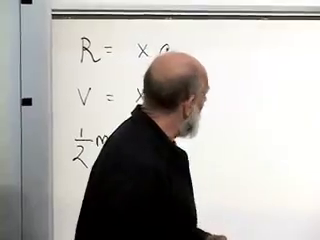
\includegraphics[width=0.72\textwidth]{lecture_09_figure_02.png}
  \caption{Metric phẳng đang giãn nở, với hệ số tỉ lệ nhân vào phần tử độ dài không gian Euclid. Khung hình nguồn tại 00:09:12.}
  \label{fig:l09-expanding-metric-board}
\end{figure}

Hãy tưởng tượng các tọa độ được vẽ trên một tấm cao su. Các dấu tọa độ vẫn gắn với tấm đó trong khi khoảng cách vật lý giữa chúng tăng lên. Vì thế, một hiệu tọa độ như "từ \(x=0\) đến \(x=1\)" chỉ là một cặp nhãn. Khoảng cách mà khoảng đó biểu diễn là \(a(t)\). Tìm phương trình chi phối hệ số tỉ lệ này là bài toán động lực học của bài giảng.

\section{Các hình học không gian kín, phẳng và mở}

Tính phẳng là một sự đơn giản hóa do quan sát, không phải là hệ quả của tính đồng nhất. Có ba hình học không gian vừa đồng nhất vừa đẳng hướng: độ cong dương, bằng 0 và âm. Để hiểu trường hợp dương, cần nói chính xác về số chiều.

Quỹ tích
\begin{equation}
  X_1^2+X_2^2=R^2
\end{equation}
là một đường tròn, hay mặt cầu một chiều \(S^1\). Phần trong đặc của nó là một đĩa, còn gọi là quả cầu hai chiều. Thêm một tọa độ nhúng nữa ta được
\begin{equation}
  X_1^2+X_2^2+X_3^2=R^2,
\end{equation}
mặt cầu hai chiều thông thường \(S^2\). Thêm một tọa độ nhúng thứ tư ta được
\begin{equation}
  X_1^2+X_2^2+X_3^2+X_4^2=R^2,
  \label{eq:l09-three-sphere}
\end{equation}
một mặt cầu ba chiều \(S^3\), bản thân nó là một không gian ba chiều. Ta không thể hình dung phép nhúng bốn chiều của nó, nhưng hình học nội tại không cần phép nhúng ấy để tồn tại.

\begin{figure}[H]
  \centering
  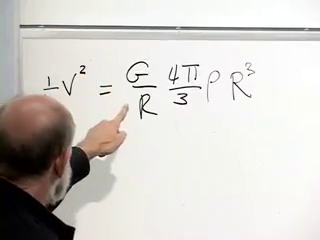
\includegraphics[width=0.72\textwidth]{lecture_09_figure_03.png}
  \caption{Phương trình nhúng dùng để giới thiệu mặt cầu ba chiều. Khung hình nguồn tại 00:16:40.}
  \label{fig:l09-three-sphere-board}
\end{figure}

Mọi điểm trên một mặt cầu lý tưởng đều tương đương về mặt hình học với mọi điểm khác, và mọi hướng tại một điểm đều tương đương. Vì thế, một mặt cầu vừa đồng nhất vừa đẳng hướng. Nếu bán kính của nó được nhân với \(a(t)\), toàn bộ không gian sẽ giãn ra hoặc co lại mà không chọn ra một tâm nào trên mặt cầu. Lần ngược một vũ trụ như vậy về quá khứ không đặt toàn bộ vật chất vào một vị trí đặc biệt nào trong một khoảng trống bên ngoài. Toàn bộ không gian trở nên nhỏ lại, nên mọi cặp điểm đều trở nên gần nhau. Vụ Nổ Lớn không phải là một vụ nổ từ một điểm của không gian.

Trên một mặt cầu có độ cong dương, các tam giác trắc địa có tổng góc lớn hơn \(180^\circ\). Các tam giác phẳng có tổng góc đúng bằng \(180^\circ\). Trong một hình học đồng nhất có độ cong âm, được biểu diễn không hoàn hảo bằng một mặt yên ngựa, tổng góc nhỏ hơn \(180^\circ\). Các phép kiểm tra nội tại này phân biệt ba trường hợp.

\begin{figure}[H]
  \centering
  \includegraphics[width=0.72\textwidth]{lecture_09_figure_07.png}
  \caption{Độ cong dương, bằng 0 và âm được phác họa qua các dạng tam giác đặc trưng của chúng. Khung hình nguồn tại 00:37:30.}
  \label{fig:l09-curvature-board}
\end{figure}

Một metric cục bộ phẳng hoàn toàn tự nó không chứng minh rằng không gian là vô hạn về tô pô. Các tô pô phẳng compact là khả dĩ về mặt toán học, mặc dù bài giảng dùng mô hình Euclid vô hạn đơn giản nhất.
\editorialnote{Bảo lưu về tô pô toàn cục này không cần đến cho bất kỳ động lực học cục bộ nào về sau.}

\section{Nhãn đồng chuyển động và định luật Hubble}

Bây giờ hãy trở lại tấm phẳng đang giãn nở và vẽ lên đó một lưới tọa độ. Trong tọa độ đồng chuyển động, lưới này giãn nở cùng với dòng vật chất quy mô lớn. Một thiên hà, hay chính xác hơn là một cụm thiên hà được làm trơn ở thang đủ thô, giữ một nhãn tọa độ xấp xỉ cố định mặc dù khoảng cách vật lý của nó tới một vật thể đồng chuyển động khác thay đổi.

\begin{figure}[H]
  \centering
  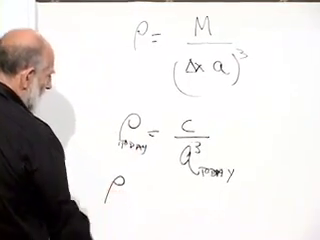
\includegraphics[width=0.72\textwidth]{lecture_09_figure_04.png}
  \caption{Một lưới tọa độ được mang theo bởi một tấm không gian đang giãn nở. Khung hình nguồn tại 00:22:20.}
  \label{fig:l09-comoving-grid-board}
\end{figure}

Đối với hai vật thể cách nhau dọc theo trục \(x\) bởi một khoảng đồng chuyển động cố định \(\Delta x\), khoảng cách vật lý của chúng là
\begin{equation}
  D(t)=a(t)\,\Delta x.
  \label{eq:l09-physical-distance}
\end{equation}
Lấy đạo hàm trong khi giữ \(\Delta x\) cố định, ta được
\begin{equation}
  v(t)=\dot a(t)\,\Delta x
      =\frac{\dot a(t)}{a(t)}D(t).
\end{equation}
Định nghĩa
\begin{equation}
  H(t)\equiv\frac{\dot a(t)}{a(t)},
  \label{eq:l09-hubble-parameter}
\end{equation}
ta thu được định luật Hubble,
\begin{equation}
  v=H(t)D.
  \label{eq:l09-hubble-law}
\end{equation}
Từ "hằng số" trong "hằng số Hubble" có nghĩa là không đổi theo không gian tại một thời điểm vũ trụ xác định. Nó không hàm ý tính không đổi trong suốt lịch sử vũ trụ.

\begin{figure}[H]
  \centering
  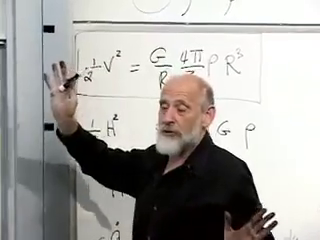
\includegraphics[width=0.72\textwidth]{lecture_09_figure_05.png}
  \caption{Phép suy ra trên bảng \(D=a\Delta x\),
  \(v=(\dot a/a)D=HD\). Khung hình nguồn tại 00:26:40.}
  \label{fig:l09-hubble-board}
\end{figure}

\begin{classroomqa}
\audiencequestion{Nếu một thiên hà xa được quan sát ở một thời điểm sớm hơn, liệu tham số Hubble suy ra cho nó có thật sự bằng giá trị được đo ở gần chúng ta ngày nay không?}
\lecturerresponse{Chỉ khi thời gian nhìn lùi nhỏ so với tuổi của vũ trụ. Ở các khoảng cách vừa phải, \(H(t)\) biến thiên đủ ít để một con số vẫn hữu ích. Ở các khoảng cách thật sự vũ trụ học, ta nhìn thấy những kỷ nguyên sớm hơn, và phải tính đến sự phụ thuộc theo thời gian của \(a\) và \(H\). Đó là một lý do khiến ta cần một phương trình động lực học cho hệ số tỉ lệ.}
\end{classroomqa}

\section{Tia null trong một hệ tọa độ đang giãn nở}

\begin{classroomqa}
\audiencequestion{Hệ số tỉ lệ có ảnh hưởng đến sự truyền ánh sáng giữa các thiên hà xa không?}
\lecturerresponse{Một tia sáng đi theo một quỹ đạo null, nên \(d\tau=0\). Đối với một tia chuyển động dọc theo trục \(x\) dương, \(dy=dz=0\), và metric giãn nở cho
\begin{align}
  0&=dt^2-a^2(t)dx^2,
  &dt&=a(t)dx,\notag\\
  &&\frac{dx}{dt}&=\frac{1}{a(t)}.
  \label{eq:l09-null-ray}
\end{align}
Vận tốc tọa độ giảm khi \(a(t)\) tăng, nhưng tốc độ ánh sáng vật lý cục bộ vẫn là \(c=1\). Một khoảng tọa độ cố định biểu diễn một khoảng cách vật lý ngày càng lớn.}
\end{classroomqa}

\begin{figure}[H]
  \centering
  \includegraphics[width=0.72\textwidth]{lecture_09_figure_06.png}
  \caption{Điều kiện null và \(dt=a(t)dx\) đối với sự truyền ánh sáng xuyên tâm. Khung hình nguồn tại 00:30:54.}
  \label{fig:l09-null-board}
\end{figure}

Người ta có thể chọn các tọa độ trong đó cùng một sự kiện này được diễn đạt như "ánh sáng chậm đi khi ở xa hơn", nhưng khi ấy các độ dài và đồng hồ lại nhận những mô tả tương ứng vụng về. Cách nói không gian giãn nở gọn hơn vì nó bảo toàn phát biểu cục bộ rằng mọi quan sát viên rơi tự do đều đo cùng một tốc độ ánh sáng.

\begin{classroomqa}
\audiencequestion{Có bằng chứng nào cho thấy sự truyền ánh sáng cục bộ và vật lý nguyên tử là như nhau trong các thiên hà xa không?}
\lecturerresponse{Chỉ những so sánh không thứ nguyên mới có ý nghĩa thao tác. Hãy chọn một kích thước nguyên tử làm đơn vị độ dài và một chu kỳ nguyên tử hoặc hạt nhân làm đơn vị thời gian, rồi hỏi ánh sáng cần bao nhiêu chu kỳ như vậy để đi qua độ dài đã chọn. Các quan sát quang phổ ủng hộ khẳng định rằng các tỉ số không thứ nguyên này là như nhau ở các vùng xa. Bằng chứng là gián tiếp, nhưng đó chính xác là kiểu so sánh dùng để kiểm tra tính đồng nhất của các định luật cục bộ.}
\end{classroomqa}

Khi vũ trụ quan sát được cực kỳ nhỏ, ánh sáng có thể băng qua một miền vật lý cho trước rất nhanh nếu đo bằng đơn vị thời gian ánh sáng băng qua tương ứng. Điều này không có nghĩa là \(c\) đã khác. Nó có nghĩa là chính miền đó khi ấy nhỏ.

\section{Một hình cầu Newton bên trong vũ trụ}

Bây giờ ta chuyển từ động học sang động lực học. Hãy đặt mình tại gốc tọa độ và vẽ một hình cầu đủ lớn để chứa nhiều thiên hà và cụm thiên hà. Chọn một thiên hà trên biên của nó. Trong một vũ trụ đồng nhất, phân bố khối lượng là đối xứng cầu quanh ta, và định lý vỏ cầu của Newton cho hai sự kiện then chốt:
\begin{enumerate}
  \item mọi vật chất được phân bố cầu ở ngoài bán kính đã chọn tác dụng lực Newton tổng cộng bằng 0 lên thiên hà ở biên;
  \item mọi vật chất ở bên trong hình cầu tác dụng, đối với chuyển động theo phương bán kính này, như thể nó tập trung tại tâm.
\end{enumerate}
Ta dùng một hệ quy chiếu trong đó ta đứng yên, nên các vận tốc và gia tốc trong lập luận sau đây được đo tương đối so với ta.

\begin{figure}[H]
  \centering
  \includegraphics[width=0.72\textwidth]{lecture_09_figure_08.png}
  \caption{Cấu dựng theo định lý vỏ cầu: ta ở tâm và một thiên hà thử trên biên của một hình cầu đồng nhất lớn. Khung hình nguồn tại 00:41:10.}
  \label{fig:l09-shell-board}
\end{figure}

\begin{figure}[H]
  \centering
  \begin{tikzpicture}[scale=0.92,>=Latex]
    \draw[thick] (0,0) circle (2.35);
    \fill (0,0) circle (2pt) node[below left] {us};
    \fill (2.35,0) circle (2.2pt) node[right] {test galaxy \(m\)};
    \draw[->,thick,blue!65!black] (0.18,0) -- (2.15,0)
      node[midway,above] {\(R=a(t)x\)};
    \draw[->,thick,red!65!black] (2.35,0.12) -- (3.25,0.12)
      node[midway,above] {\(v=\dot a(t)x\)};
    \node[align=center,text width=7cm] at (0,-2.85)
      {outside shells cancel;\\enclosed mass acts at the center};
  \end{tikzpicture}
  \caption{Phục dựng gọn của cấu dựng Newton.}
  \label{fig:l09-shell-clean}
\end{figure}

Nếu thiên hà có tọa độ đồng chuyển động cố định \(x\), thì bán kính vật lý và vận tốc của nó là
\begin{equation}
  R(t)=x a(t),
  \qquad
  v(t)=x\dot a(t)=H(t)R(t).
  \label{eq:l09-radius-velocity}
\end{equation}
Gọi \(M\) là khối lượng bao trong hình cầu và \(m\) là khối lượng của thiên hà thử. Năng lượng Newton là
\begin{equation}
  E=\frac12 m v^2-\frac{GMm}{R}.
  \label{eq:l09-newtonian-energy}
\end{equation}

\begin{figure}[H]
  \centering
  \includegraphics[width=0.72\textwidth]{lecture_09_figure_09.png}
  \caption{Toàn bộ chuỗi suy ra trên bảng \(R=xa\), \(v=x\dot a\), và phương trình năng lượng Newton được chuyên biệt hóa cho \(E=0\). Khung hình nguồn tại 00:48:40.}
  \label{fig:l09-energy-board}
\end{figure}

Năng lượng có thể dương, bằng 0 hoặc âm. Hãy bắt đầu ở ranh giới giữa thoát ly và co sụp trở lại, \(E=0\), khi đó
\begin{equation}
  \frac12 v^2=\frac{GM}{R}.
  \label{eq:l09-zero-energy}
\end{equation}

\begin{classroomqa}
\audiencequestion{Tổng năng lượng bằng 0 có nghĩa gì đối với thiên hà đang lùi ra xa?}
\lecturerresponse{Đó chính xác là trường hợp vận tốc thoát. Năng lượng dương nghĩa là chuyển động vượt vận tốc thoát; năng lượng âm nghĩa là chuyển động dưới vận tốc thoát và, trong bức tranh Newton chỉ gồm vật chất, là cuối cùng quay trở lại. Ta bắt đầu ở ranh giới giữa các khả năng đó và sẽ quay lại các dấu kia sau khi suy ra phương trình phẳng.}
\end{classroomqa}

\begin{classroomqa}
\audiencequestion{Liệu \(M\), khối lượng bao trong, có biến thiên khi hình cầu giãn nở không?}
\lecturerresponse{Không. Hình cầu là đồng chuyển động, nên vẫn chính những hạt ấy ở bên trong nó. Thể tích vật lý của nó tăng lên và mật độ của nó giảm xuống, nhưng tổng khối lượng bao trong vẫn giữ cố định. Sự phân biệt này giữa \(M\) và \(\rho(t)\) là thiết yếu.}
\end{classroomqa}

Với mật độ đồng nhất \(\rho(t)\),
\begin{equation}
  M=\frac{4\pi}{3}\rho(t)R^3.
  \label{eq:l09-enclosed-mass}
\end{equation}
Thay vào \eqref{eq:l09-zero-energy} ta được
\begin{equation}
  \frac12 v^2
  =\frac{G}{R}\left(\frac{4\pi}{3}\rho R^3\right).
  \label{eq:l09-enclosed-energy}
\end{equation}

\begin{figure}[H]
  \centering
  \includegraphics[width=0.72\textwidth]{lecture_09_figure_10.png}
  \caption{Phép thay thế bằng khối lượng chứa bên trong trong phương trình năng lượng bằng 0.
  Khung hình nguồn tại 00:54:16.060.}
  \label{fig:l09-enclosed-mass-board}
\end{figure}

Dùng \(v=HR\), ta được
\begin{align}
  \frac12 H^2R^2
    &=\frac{4\pi G}{3}\rho R^2,\\
  H^2
    &=\frac{8\pi G}{3}\rho.
\end{align}
Do đó, định luật giãn nở năng lượng bằng 0, phẳng theo không gian là
\begin{equation}
  \boxed{\left(\frac{\dot a}{a}\right)^2
  =\frac{8\pi G}{3}\rho(t)}.
  \label{eq:l09-flat-friedmann}
\end{equation}
Sự triệt tiêu của \(R^2\) không phải là ngẫu nhiên. Một vũ trụ đồng nhất phải
cho cùng \(H(t)\) bất kể thiên hà đồng chuyển động nào được chọn làm vật thử.

\begin{figure}[H]
  \centering
  \includegraphics[width=0.72\textwidth]{lecture_09_figure_11.png}
  \caption{Sự triệt tiêu của bán kính và hệ thức Friedmann phẳng thu được trên bảng.
  Khung hình nguồn tại 00:57:30.}
  \label{fig:l09-friedmann-board}
\end{figure}

\begin{classroomqa}
\audiencequestion{Có bằng chứng nào cho hệ thức năng lượng bằng 0 không?}
\lecturerresponse{Cả hai vế đều có thể được suy ra từ quan sát: \(H\) từ
dữ liệu lùi xa và \(\rho\) bằng cách tính đến sao, khí, vật chất tối và
năng lượng chân không. Phép so sánh vào thời điểm bài giảng cho thấy hai vế
phù hợp với nhau ở mức chính xác cỡ phần trăm. Điều bảo lưu này rất quan
trọng: phải bao gồm mọi dạng năng lượng, và phần thảo luận sau về năng lượng
chân không làm thay đổi cách diễn giải ngây thơ theo vận tốc thoát.}
\end{classroomqa}

Trong hệ đơn vị \(c=1\), mật độ khối lượng và mật độ năng lượng có cùng đơn vị. Ký
hiệu \(\rho\) vì thế sẽ chỉ tổng mật độ năng lượng thích hợp với thành phần đang
được bàn tới.

\section{Vật chất thông thường và quy luật hai phần ba}

Phương trình \eqref{eq:l09-flat-friedmann} chưa khép kín cho đến khi ta biết
\(\rho(t)\) biến thiên như thế nào. Trước hết hãy lấp đầy một hộp chữ nhật đồng
chuyển động bằng các hạt chuyển động chậm, phi tương đối tính. Các kích thước
tọa độ của nó là cố định, còn thể tích vật lý tăng theo
\begin{equation}
  V(t)=a^3(t)\,\Delta x\,\Delta y\,\Delta z.
\end{equation}
Số hạt và khối lượng nghỉ trong hộp giữ nguyên, nên
\begin{equation}
  \rho_{\mathrm m}(t)=\frac{C_{\mathrm m}}{a^3(t)}.
  \label{eq:l09-matter-dilution}
\end{equation}
Chuẩn hóa theo thời điểm hiện tại \(t_0\),
\begin{equation}
  \frac{\rho_{\mathrm m}(t)}{\rho_{\mathrm m,0}}
  =\left(\frac{a_0}{a(t)}\right)^3.
  \label{eq:l09-matter-normalized}
\end{equation}

\begin{figure}[H]
  \centering
  \includegraphics[width=0.72\textwidth]{lecture_09_figure_12.png}
  \caption{Mật độ vật chất, sự pha loãng \(a^{-3}\) của nó và chuẩn hóa
  ở thời điểm hiện nay. Khung hình nguồn tại 01:04:47.940.}
  \label{fig:l09-density-board}
\end{figure}

\begin{classroomqa}
\audiencequestion{Mật độ năng lượng hiện nay của vũ trụ xấp xỉ là bao nhiêu,
và chỉ riêng các nguyên tử thông thường có thể cung cấp nó không?}
\lecturerresponse{Việc đếm vật chất baryon nhìn thấy được chỉ cho một phần
câu trả lời. Vật chất tối và năng lượng tối cũng phải được biểu diễn dưới dạng
khối lượng-năng lượng tương đương. Bài giảng nêu một thang xấp xỉ trải từ một
nguyên tử đến vài chục tương đương khối lượng hydro trên mỗi mét khối, nhấn
mạnh bậc độ lớn hơn là một kiểm kê chính xác.}
\end{classroomqa}

Thế \eqref{eq:l09-matter-dilution} vào
\eqref{eq:l09-flat-friedmann} và gộp mọi thừa số không phụ thuộc thời gian vào một hằng số
dương \(C\):
\begin{equation}
  \left(\frac{\dot a}{a}\right)^2=\frac{C}{a^3},
  \qquad
  \dot a^2=\frac{C}{a}.
  \label{eq:l09-matter-ode}
\end{equation}
Có hai cách minh bạch để giải nó. Một phép thử dạng lũy thừa
\(a=K t^p\) đòi hỏi
\begin{equation}
  p-1=-\frac{p}{2},
  \qquad p=\frac23.
\end{equation}
Tương đương, chọn nhánh căn bậc hai ứng với giãn nở và tích phân:
\begin{equation}
  a^{1/2}\frac{da}{dt}=\sqrt C,
  \qquad
  \int a^{1/2}da=\sqrt C\int dt,
\end{equation}
nên, sau khi chọn gốc thời gian tại Big Bang,
\begin{equation}
  a^{3/2}\propto t,
  \qquad
  \boxed{a(t)\propto t^{2/3}}.
  \label{eq:l09-matter-solution}
\end{equation}
Trong phép suy dẫn trực tiếp, có lúc tạm thời làm mất một thừa số khi ghép hệ
số, rồi quay lại phép tích phân và kiểm tra số mũ. Ghi chú giữ lại phép kiểm
tra nhưng chỉ trình bày đại số đã hiệu chỉnh.

\begin{figure}[H]
  \centering
  \includegraphics[width=0.72\textwidth]{lecture_09_figure_13.png}
  \caption{Phép thử dạng lũy thừa và số mũ được đóng khung \(p=2/3\). Khung hình nguồn
  tại 01:13:05.}
  \label{fig:l09-matter-solution-board}
\end{figure}

Lấy đạo hàm của nghiệm cho
\begin{equation}
  H(t)=\frac{\dot a}{a}=\frac{2}{3t}.
  \label{eq:l09-matter-hubble}
\end{equation}
Tham số Hubble trong quá khứ lớn hơn. Do đó, khi nhìn đủ xa để thấy thời gian
nhìn lùi đáng kể, ta không nên kéo dài quan hệ tuyến tính cục bộ mà vẫn giữ
nguyên \(H_0\) hiện nay.

\begin{figure}[H]
  \centering
  \includegraphics[width=0.72\textwidth]{lecture_09_figure_14.png}
  \caption{Lấy \(\dot a/a\) của \(a\propto t^{2/3}\) cho
  \(H=2/(3t)\). Khung hình nguồn tại 01:20:42.}
  \label{fig:l09-hubble-time-board}
\end{figure}

\section{Dấu của năng lượng và độ cong không gian}

Lập luận kiểu Newton đã đưa ta đi qua trường hợp phẳng có năng lượng bằng 0. Thuyết
 tương đối rộng bổ sung một sự kiện không thể thu được chỉ từ định lý vỏ cầu:
dấu của năng lượng riêng kiểu Newton tương ứng với dấu của độ cong không
gian.
\begin{center}
\begin{tabular}{@{}>{\raggedright\arraybackslash}p{0.20\linewidth}
                    >{\raggedright\arraybackslash}p{0.29\linewidth}
                    >{\raggedright\arraybackslash}p{0.37\linewidth}@{}}
  \toprule
  Tổng năng lượng & Độ cong không gian & Số phận khi chỉ có vật chất \\
  \midrule
  dương & âm (mở) & giãn nở mãi mãi \\
  bằng 0 & bằng 0 (phẳng) & tiệm cận ngưỡng thoát \\
  âm & dương (đóng) & giãn nở, quay đầu, tái co sụp \\
  \bottomrule
\end{tabular}
\end{center}
Cột cuối giả sử không có năng lượng chân không. Trong phép tương tự vật phóng, năng lượng
dương nghĩa là trên vận tốc thoát, bằng 0 nghĩa là đúng bằng vận tốc thoát,
và âm nghĩa là dưới vận tốc thoát. Các phương trình Einstein đồng nhất ba
trường hợp này lần lượt với hình học không gian mở, phẳng và đóng.

\section{Photon và quy luật một phần hai}

Quy luật vật chất \(\rho\propto a^{-3}\) giả sử rằng năng lượng của mỗi hạt
xấp xỉ cố định trong khi mật độ số giảm xuống. Photon vi phạm giả định đó.
Đối với một photon,
\begin{equation}
  E=h\nu=\frac{hc}{\lambda}.
\end{equation}
Sự giãn nở làm bước sóng của nó dãn ra tỉ lệ với thừa số tỉ lệ,
\begin{equation}
  \lambda\propto a,
  \qquad E\propto a^{-1}.
\end{equation}
Mật độ số photon vẫn giảm như \(a^{-3}\), và năng lượng của mỗi photon đóng
góp thêm một thừa số \(a^{-1}\). Vì vậy
\begin{equation}
  \boxed{\rho_{\mathrm r}(t)\propto a^{-4}(t)}.
  \label{eq:l09-radiation-dilution}
\end{equation}

Phép tương tự dây đàn guitar nắm bắt bức tranh vật lý. Gảy một dây rồi kéo
dài phần đang dao động của nó: bước sóng dài ra và cao độ hạ xuống. Một mode
photon trong một hộp đồng chuyển động đang giãn nở cũng hành xử tương tự. Nếu
chạy ngược bức tranh, sự nén lại làm bước sóng ngắn đi và năng lượng photon
tăng lên.

\begin{figure}[H]
  \centering
  \includegraphics[width=0.72\textwidth]{lecture_09_figure_15.png}
  \caption{Hệ thức mật độ vật chất được mở rộng trên bảng thành
  quy luật tỉ lệ của bức xạ \(\rho_{\mathrm r}\propto a^{-4}\). Khung hình nguồn tại 01:29:20.}
  \label{fig:l09-radiation-board}
\end{figure}

Dùng \(\rho_{\mathrm r}\propto a^{-4}\) trong phương trình Friedmann phẳng, ta được
\begin{equation}
  \left(\frac{\dot a}{a}\right)^2=\frac{C_{\mathrm r}}{a^4},
  \qquad
  \dot a\propto a^{-1},
\end{equation}
và do đó
\begin{equation}
  \boxed{a(t)\propto t^{1/2}}.
  \label{eq:l09-radiation-solution}
\end{equation}
Nó tăng chậm hơn \(t^{2/3}\). Đi đủ xa về quá khứ, bức xạ tất phải trội hơn vật
chất thông thường vì \(a^{-4}\) tăng nhanh hơn \(a^{-3}\) khi \(a\) giảm.
Bài giảng đặt thời điểm chuyển tiếp vật chất-bức xạ vào khoảng khi thừa số tỉ
lệ nhỏ hơn hiện nay chừng một nghìn lần. Trước mốc chuyển tiếp đó, vũ trụ bị
bức xạ chi phối; sau đó, trong một khoảng dài, nó bị vật chất chi phối.

\section{Năng lượng chân không và giãn nở hàm mũ}

Năng lượng chân không có hành vi tỉ lệ hóa ngược lại. Mật độ của nó là một
thuộc tính của không gian trống và không bị pha loãng khi vũ trụ giãn nở:
\begin{equation}
  \rho_\Lambda=\text{constant}.
  \label{eq:l09-vacuum-density}
\end{equation}
Vật chất thông thường và bức xạ trở nên đậm đặc hơn khi đi về quá khứ, còn hạng
này thì không. Vì thế nó kém quan trọng hơn trong vũ trụ sơ khai và trở nên
quan trọng hơn khi các thành phần khác bị pha loãng. Bài giảng dùng ước lượng
đương thời rằng năng lượng chân không chiếm khoảng \(70\%\) mật độ năng lượng
vũ trụ hiện nay.

Với \(\rho_\Lambda\) không đổi, phương trình \eqref{eq:l09-flat-friedmann} cho một
tốc độ giãn nở không đổi
\begin{equation}
  H_\Lambda=\sqrt{\frac{8\pi G}{3}\rho_\Lambda},
  \qquad
  \frac{\dot a}{a}=H_\Lambda.
\end{equation}
Do đó
\begin{equation}
  \boxed{a(t)=a(t_i)e^{H_\Lambda(t-t_i)}}.
  \label{eq:l09-vacuum-solution}
\end{equation}

\begin{figure}[H]
  \centering
  \includegraphics[width=0.72\textwidth]{lecture_09_figure_16.png}
  \caption{Phương trình mật độ không đổi dẫn đến giãn nở hàm mũ.
  Khung hình nguồn tại 01:35:48.}
  \label{fig:l09-vacuum-board}
\end{figure}

Ở thang quan sát được nêu trong bài giảng, vũ trụ tăng gấp đôi kích thước tuyến tính trong khoảng chừng mười đến mười hai tỷ năm. Nguồn gốc của mật độ chân không nhỏ nhưng khác không này vẫn chưa được giải thích; sự tồn tại của nó cùng ảnh hưởng của nó đối với sự giãn nở là những dữ kiện thực nghiệm.

\begin{classroomqa}
\audiencequestion{Trong phần bàn luận này, năng lượng chân không có phải chính là năng lượng tối không?}
\lecturerresponse{Có. Ở đây “năng lượng tối” chỉ một mật độ năng lượng chân
không không đổi, tương đương với một hằng số vũ trụ học. Có thể hình dung
những mô hình năng lượng tối tổng quát hơn, phụ thuộc thời gian, nhưng chúng
không thuộc phép tính của bài giảng này.}
\end{classroomqa}

\section{Vũ trụ giãn nở làm dịch đỏ ánh sáng như thế nào}

\begin{classroomqa}
\audiencequestion{Làm sao photon có thể biết rằng ta đã chọn các tọa độ đồng
chuyển động đang giãn nở và vì thế làm giảm năng lượng của chúng?}
\lecturerresponse{Chúng không phản ứng với các nhãn của ta. Chúng lan truyền
trong một hình học mà các khoảng cách vật lý thay đổi. Một đoàn sóng chiếm
một vùng có kích thước vật lý tăng gấp đôi sẽ có bước sóng tăng gấp đôi. Các
tọa độ đồng chuyển động chỉ mô tả sự kéo giãn này một cách gọn gàng; chúng
không gây ra nó.}
\end{classroomqa}

\begin{classroomqa}
\audiencequestion{Các photon nền đến với ta ngày nay xuất phát từ đâu?}
\lecturerresponse{Nhìn càng xa nghĩa là nhìn càng sớm. Rồi đến lúc ta thấy
thời kỳ mà vật chất vũ trụ là một plasma ion hóa, mờ đục vì photon tán xạ lặp
đi lặp lại trên các hạt mang điện tự do. Biên mà từ đó photon lần cuối có thể
truyền tự do đến ta hiện ra như một mặt cầu bao quanh người quan sát: bề mặt
tán xạ cuối cùng.}
\end{classroomqa}

\begin{figure}[H]
  \centering
  \includegraphics[width=0.72\textwidth]{lecture_09_figure_17.png}
  \caption{Phác họa lấy người quan sát làm tâm của bề mặt tán xạ cuối cùng và
  các lớp vỏ ở xa dần. Khung hình nguồn tại 01:42:05.}
  \label{fig:l09-last-scattering-board}
\end{figure}

\begin{figure}[H]
  \centering
  \begin{tikzpicture}[scale=0.9,>=Latex]
    \fill (0,0) circle (2pt) node[below] {observer};
    \draw[thick,orange!70!black] (0,0) circle (2.55);
    \node[orange!70!black,align=center] at (0,3.05)
      {surface of last scattering};
    \foreach \a in {25,75,145,210,285,335}{
      \draw[->,blue!60!black] ({2.55*cos(\a)},{2.55*sin(\a)}) --
        ({1.7*cos(\a)},{1.7*sin(\a)});
    }
    \draw[decorate,decoration={snake,amplitude=1.5pt,segment length=7pt},
      red!65!black,thick,->] (-2.5,0) -- (-0.15,0);
    \node[red!65!black,below] at (-1.35,-0.15)
      {redshifted photon};
  \end{tikzpicture}
  \caption{Bản dựng lại rõ ràng của bức tranh tán xạ cuối cùng.}
  \label{fig:l09-last-scattering-clean}
\end{figure}

Bức xạ được phát ra với phổ đặc trưng của một plasma nóng và đến với ta với
bước sóng dài hơn xấp xỉ một nghìn lần. Theo ngôn ngữ Doppler của bài giảng,
bề mặt phát xạ ở xa lùi ra nhanh và bức xạ của nó bị dịch đỏ mạnh. Theo ngôn
ngữ hình học, sóng bị kéo giãn trong quá trình lan truyền. Cả hai cách nhìn
đều mã hóa cùng một hệ thức,
\begin{equation}
  1+z=\frac{\lambda_0}{\lambda_{\mathrm{em}}}
      =\frac{a_0}{a_{\mathrm{em}}}.
  \label{eq:l09-cosmological-redshift}
\end{equation}
\editorialnote{Phương trình \eqref{eq:l09-cosmological-redshift} là dạng định lượng chuẩn của các mô tả
kéo giãn và Doppler trong bài giảng.}

Ở một thời điểm quan sát sớm hơn, mặt cầu tán xạ cuối cùng trong bức tranh
tương ứng sẽ ở gần hơn, và các photon nền quan sát được sẽ bị dịch đỏ ít hơn
nên giàu năng lượng hơn. Khi thời gian vũ trụ trôi đi, các photon đi tới một
người quan sát đồng chuyển động từ plasma sơ khai ấy có bước sóng ngày càng
dài hơn.

\section{Năng lượng của một photon bị dịch đỏ đi đâu?}

\begin{classroomqa}
\audiencequestion{Một photon được phát ra với năng lượng \(h\nu_{\mathrm{em}}\) và
đến nơi trong trạng thái bị dịch đỏ với năng lượng nhỏ hơn. Điều gì đã xảy ra
với phần chênh lệch?}
\lecturerresponse{Phép suy dẫn kiểu Newton khởi đầu từ một phương trình năng
lượng. Dạng vũ trụ học của nó liên hệ tốc độ giãn nở với mật độ năng lượng vật
chất, nên không thể xem năng lượng của vật chất và sự giãn nở như những sổ cái
bảo toàn tách biệt. Bài giảng mô tả phần năng lượng photon bị mất là đi vào
phần hạch toán động năng của sự giãn nở. Một pít-tông chứa đầy bức xạ làm phép
tương tự trở nên cụ thể: áp suất bức xạ đẩy pít-tông ra ngoài, bước sóng photon
tăng lên, và phần năng lượng bị mất của chúng trở thành công cơ học và động năng
của pít-tông.}
\end{classroomqa}

\begin{figure}[H]
  \centering
  \includegraphics[width=0.72\textwidth]{lecture_09_figure_18.png}
  \caption{Trên bảng, phương trình năng lượng kiểu Newton được đóng khung nằm phía trên
  phương trình Friedmann tương ứng. Khung hình nguồn tại 01:44:42.}
  \label{fig:l09-energy-bookkeeping-board}
\end{figure}

\begin{classroomqa}
\audiencequestion{Điều gì ghép nối năng lượng bức xạ với sự giãn nở?}
\lecturerresponse{Áp suất. Trong một xi lanh với pít-tông di động, photon
truyền động lượng cho thành. Khi pít-tông chuyển động, bức xạ thực hiện công;
bước sóng của nó tăng lên và năng lượng của nó giảm xuống. Vũ trụ đồng nhất
đang giãn nở không có một pít-tông ngoài theo nghĩa đen, nhưng phép tương tự
\(p\,dV\) giải thích vì sao mật độ năng lượng của bức xạ giảm nhanh hơn so với
chỉ do sự pha loãng số lượng.}
\end{classroomqa}

\begin{figure}[H]
  \centering
  \includegraphics[width=0.72\textwidth]{lecture_09_figure_19.png}
  \caption{Pít-tông di động chứa photon được dùng để hình dung công áp suất.
  Khung hình nguồn tại 01:46:40.}
  \label{fig:l09-piston-board}
\end{figure}

\begin{figure}[H]
  \centering
  \begin{tikzpicture}[scale=0.92,>=Latex]
    \draw[thick] (0,0) rectangle (5.3,2.6);
    \draw[very thick] (4.25,0) -- (4.25,2.6);
    \draw[very thick] (4.25,1.3) -- (5.25,1.3);
    \draw[->,thick,red!65!black] (5.25,1.3) -- (6.2,1.3)
      node[right] {moving piston};
    \foreach \y in {0.55,1.3,2.05}{
      \draw[decorate,decoration={snake,amplitude=1.4pt,segment length=6pt},
        blue!65!black,->] (0.35,\y) -- (3.9,\y);
    }
    \node at (2.15,-0.45) {radiation does \(p\,dV\) work};
  \end{tikzpicture}
  \caption{Bản dựng lại rõ ràng của phép tương tự bức xạ–pít-tông.}
  \label{fig:l09-piston-clean}
\end{figure}

Năng lượng trong thuyết tương đối rộng đòi hỏi phải cẩn trọng. Trong một không-thời gian giãn nở tổng quát, không nhất thiết tồn tại một năng lượng toàn cục được bảo toàn duy nhất tương tự như năng lượng của một hệ Newton cô lập. Sự bảo toàn cục bộ năng lượng-động lượng vẫn đúng, và đối với một lưu chất đồng nhất, nó cho phương trình liên tục
\begin{equation}
  \dot\rho+3H(\rho+p)=0,
  \label{eq:l09-continuity}
\end{equation}
phương trình này chứa hạng công do áp suất đứng sau các định luật tỉ lệ của vật chất và bức xạ.\editorialnote{Phương trình \eqref{eq:l09-continuity} là phát biểu cục bộ chính xác của thuyết tương đối rộng làm cơ sở cho phép loại suy hạch toán năng lượng có chủ ý theo kiểu Newton trong bài giảng.}

Năng lượng chân không làm cho vấn đề ấy trở nên đặc biệt sắc nét. Vì mật độ của nó giữ không đổi trong khi thể tích tăng, tổng năng lượng chân không trong một vùng đồng chuyển động tăng lên. Áp suất âm của nó là một phần của nguồn hấp dẫn và thúc đẩy sự giãn nở gia tốc. Vì vậy, không nên đòi hỏi khái niệm ngây thơ về "năng lượng vật chất trong một hộp đồng chuyển động" phải được bảo toàn riêng biệt mà không tính cả hình học và công do áp suất.

\section{Vì sao có thể bỏ hệ số tỉ lệ khỏi hạng thời gian}

\begin{classroomqa}
\audiencequestion{Vì sao hệ số tỉ lệ nhân với phần không gian của metric mà không nhân với phần thời gian?}
\lecturerresponse{Đó là do cách chọn tọa độ thời gian. Giả sử ta bắt đầu với tọa độ thời gian bảo giác \(t\), trong đó
\begin{equation}
  d\tau^2=A^2(t)\left(dt^2-dx^2\right).
\end{equation}
Định nghĩa một thời gian vũ trụ mới \(T\) bởi
\begin{equation}
  dT=A(t)\,dt.
\end{equation}
Khi đó
\begin{equation}
  d\tau^2=dT^2-A^2\bigl(t(T)\bigr)dx^2.
\end{equation}
Hệ số chung đứng trước vi phân thời gian đã biến mất, trong khi hệ số tỉ lệ vật lý vẫn còn ở hạng không gian.}
\end{classroomqa}

\begin{figure}[H]
  \centering
  \includegraphics[width=0.72\textwidth]{lecture_09_figure_20.png}
  \caption{Phép tái định nghĩa thời gian \(dT=A(t)dt\) chuyển từ thời gian bảo giác sang thời gian vũ trụ. Khung hình gốc tại 01:51:05.}
  \label{fig:l09-time-reparam-board}
\end{figure}

\section{Độ cong, năng lượng chân không và số phận vũ trụ}

\begin{classroomqa}
\audiencequestion{Nếu vũ trụ có độ cong dương, liệu chúng ta đã phải thấy các thiên hà đang tiến lại gần chúng ta chưa?}
\lecturerresponse{Không nhất thiết. Một vật được phóng đi với vận tốc nhỏ hơn vận tốc thoát thì ban đầu sẽ đi ra xa, đạt tới một điểm ngoặt, và chỉ về sau mới rơi trở lại. Chúng ta quan sát vũ trụ trong một pha đang giãn nở. Nếu không có năng lượng chân không, một vũ trụ vật chất có độ cong dương cuối cùng sẽ co sụp trở lại. Một năng lượng chân không dương đủ lớn ngăn sự quay đầu đó, và giá trị quan sát được dường như đủ lớn để làm cho sự giãn nở về lâu dài diễn ra theo hàm mũ, bất kể một độ cong không gian nhỏ.}
\end{classroomqa}

Tương lai hàm mũ ấy không phải là một thiên đường về năng lượng. Các ngôi sao rốt cuộc sẽ cháy hết, mật độ vật chất và bức xạ giảm theo hàm mũ, và các vùng xa xôi vượt ra ngoài liên hệ nhân quả. Năng lượng chân không vẫn còn, trong khi các cấu trúc thông thường trở nên ngày càng lạnh hơn và loãng hơn.

\begin{classroomqa}
\audiencequestion{Nhìn xa hơn vào quá khứ, có nhiều photon hơn các hạt vật chất thông thường không?}
\lecturerresponse{Tỉ số số lượng photon trên baryon đã là khổng lồ, xấp xỉ \(10^{10}\) photon trên mỗi baryon theo ước tính của bài giảng, và cả hai số lượng trong một thể tích đồng chuyển động đều gần như giữ nguyên. Điều chủ yếu thay đổi khi nhìn ngược về quá khứ là năng lượng trên mỗi photon. Năng lượng photon tăng theo \(a^{-1}\), còn khối lượng nghỉ của vật chất phi tương đối tính thì không tăng như vậy. Vì vậy, bức xạ chi phối mật độ năng lượng ở các thời điểm sớm mặc dù bản thân tỉ số số lượng ấy không nhất thiết phải thay đổi.}
\end{classroomqa}

Bài học cốt lõi là chỉ riêng hình học không quyết định lịch sử vũ trụ. Phương trình Friedmann trong trường hợp phẳng cho quan hệ giữa sự giãn nở và mật độ năng lượng, nhưng thành phần của vũ trụ quyết định sự phụ thuộc theo thời gian. Vật chất phi tương đối tính cho \(a\propto t^{2/3}\), bức xạ cho \(a\propto t^{1/2}\), còn năng lượng chân không không đổi cho sự giãn nở hàm mũ. Ba quy luật đó định hình các kỷ nguyên kế tiếp nhau của vũ trụ và giải thích vì sao cùng một hệ số tỉ lệ chi phối các khoảng cách, các độ dịch đỏ và tham số Hubble đang thay đổi.
\end{document}
